% This sample file is dedicated to the public domain.
\documentclass[12pt]{myucthesis}

%\nofiles
% The above command prevents latex from writing its auxiliary
% files. This is useful if you want to manually tweak them before you
% generate your final PDF.


% Page layout. The fancyhdr package may complain about the need for a
% larger headheight, depending on how long chapter titles are; if left
% unspecified in the geometry setup, it defaults to 12pt. The
% "showframe" option causes the geometry package (version >= 5.0) to
% show a frame around the margins on every page, which is great for
% checking that you don't overflow anywhere.

%\usepackage[letterpaper,includehead,margin=1in,headheight=15pt,showframe]{geometry}
\usepackage[letterpaper,includehead,margin=1in,headheight=15pt]{geometry}
\usepackage{fancyhdr}
\pagestyle{fancyplain}
\lhead[\fancyplain{\thepage}{\thepage}]{\fancyplain{}{\scshape\rightmark}}
\rhead[\fancyplain{}{\scshape\leftmark}]{\fancyplain{\thepage}{\thepage}}
\chead{}
\cfoot{}
\lfoot{}
\rfoot{}


% Bibliography stuff:

\newcommand{\newblock}{\par} % need this for some natbib internal bug
\bibliographystyle{abbrv}
\def\bibpreamble{\addcontentsline{toc}{chapter}{Bibliography}} % get a good TOC entry


% Other setup:

\usepackage[T1]{fontenc} % see http://tinyurl.com/67zdxwf
\usepackage[colorlinks,urlcolor=blue,citecolor=blue,linkcolor=blue,pdfusetitle]{hyperref}
\usepackage{pdflscape} % allows landscape-oriented figures with PDF page rotation
\usepackage{aasmacros,amsmath,amssymb,graphicx}
\usepackage{mydeluxetable} % deluxetable customized to play well with ucthesis

\usepackage{lmodern,microtype} % subtle typographic improvements and updated basic font

%\usepackage{times}
\usepackage{epsfig}
\usepackage{soul}
\usepackage{booktabs}
\usepackage{url}
\usepackage{mdwlist}
\usepackage{lscape}
\usepackage{array}
\usepackage{multirow}
\usepackage{rotating}
\usepackage{pifont}
\def\code#1{{\tt #1}}
% "define" Scala
\usepackage[T1]{fontenc}  
\usepackage[scaled=0.7]{beramono}  
\usepackage{microtype} 
\usepackage[procnames]{listings}

\sbox0{\small\ttfamily A}
\edef\mybasewidth{\the\wd0 }

\lstdefinelanguage{scala}{
  morekeywords={abstract,case,catch,class,def,%
    do,else,extends,false,final,finally,%
    for,if,implicit,import,match,mixin,%
    new,null,object,override,package,%
    private,protected,requires,return,sealed,%
    super,this,throw,trait,true,try,%
    type,val,var,while,with,yield,env,struct},
  sensitive=true,
  morecomment=[l]{//},
  morecomment=[n]{/*}{*/},
  morestring=[b]",
  morestring=[b]',
  morestring=[b]"""
}

\lstdefinelanguage{phdl}{
  morekeywords={module,env,struct,CtxEnv,site,assert,print},
  sensitive=true,
  morecomment=[l]{//},
  morecomment=[n]{/*}{*/},
  morestring=[b]",
  morestring=[b]',
  morestring=[b]""",
  basicstyle=\ttfamily\small,
  breaklines=true
}

\usepackage{color}
\definecolor{dkgreen}{rgb}{0,0.6,0}
\definecolor{gray}{rgb}{0.5,0.5,0.5}
\definecolor{mauve}{rgb}{0.58,0,0.82}

% Default settings for code listings
\lstset{frame=tb,
  language=scala,
  escapeinside={(*@}{@*)},
  aboveskip=0.5mm,
  belowskip=0.5mm,
  showstringspaces=false,
  columns=fixed, % basewidth=\mybasewidth,
  basicstyle={\small\ttfamily},
  numbers=none,
  numberstyle=\footnotesize\color{gray},
  % identifierstyle=\color{red},
  keywordstyle=\color{blue},
  commentstyle=\color{dkgreen},
  stringstyle=\color{mauve},
  frame=single,
  breaklines=false,
  breakatwhitespace=false,
  procnamekeys={def, val, var, class, trait, object, extends},
  procnamestyle=\ttfamily\color{red},
  tabsize=2,
  framesep=0.4pt
}
\lstnewenvironment{phdl}
{\lstset{language=phdl}}
{}
\lstnewenvironment{scala}
{\lstset{language=scala}}
{}
\lstnewenvironment{cpp}
{\lstset{language=C++}}
{}
\lstnewenvironment{bash}
{\lstset{language=bash}}
{}
\lstnewenvironment{verilog}
{\lstset{language=verilog}}
{}



% New column types to use in tabular environment for instruction formats.
% Allocate 0.18in per bit.
\newcolumntype{I}{>{\centering\arraybackslash}p{0.18in}}
% Two-bit centered column.
\newcolumntype{W}{>{\centering\arraybackslash}p{0.36in}}
% Three-bit centered column.
\newcolumntype{F}{>{\centering\arraybackslash}p{0.54in}}
% Four-bit centered column.
\newcolumntype{Y}{>{\centering\arraybackslash}p{0.72in}}
% Five-bit centered column.
\newcolumntype{R}{>{\centering\arraybackslash}p{0.9in}}
% Six-bit centered column.
\newcolumntype{S}{>{\centering\arraybackslash}p{1.08in}}
% Seven-bit centered column.
\newcolumntype{O}{>{\centering\arraybackslash}p{1.26in}}
% Eight-bit centered column.
\newcolumntype{E}{>{\centering\arraybackslash}p{1.44in}}
% Ten-bit centered column.
\newcolumntype{T}{>{\centering\arraybackslash}p{1.8in}}
% Twelve-bit centered column.
\newcolumntype{M}{>{\centering\arraybackslash}p{2.2in}}
% Sixteen-bit centered column.
\newcolumntype{K}{>{\centering\arraybackslash}p{2.88in}}
% Twenty-bit centered column.
\newcolumntype{U}{>{\centering\arraybackslash}p{3.6in}}
% Twenty-two-bit centered column.
\newcolumntype{L}{>{\centering\arraybackslash}p{3.96in}}
% Twenty-five-bit centered column.
\newcolumntype{J}{>{\centering\arraybackslash}p{4.5in}}

\newcommand{\instbit}[1]{\mbox{\scriptsize #1}}
\newcommand{\instbitrange}[2]{~\instbit{#1} \hfill \instbit{#2}~}
\newcommand{\reglabel}[1]{\hfill {\tt #1}\hfill\ }

\begin{document}
\ssp % single spacing
\hypersetup{pageanchor=false}
\title{Productive Design of Extensible On-Chip Memory Hierarchies}
\author{Henry Michael Cook} % must match BearFacts!
\degreesemester{Spring}
\degreeyear{2016}
\degree{Doctor of Philosophy}
\numberofmembers{3}
\chair{Professor David Patterson}
\othermembers{
Professor Krste Asanovi\'{c} \\
Professor Paul Wright
}
\field{Computer Science}
\campus{Berkeley}

\maketitle
\copyrightpage

\begin{abstract}
As Moore's Law slows and process scaling yields only small returns, computer architecture and design are poised to undergo a renaissance. This thesis brings the productivity of modern software tools to bear on the design of future energy-efficient hardware architectures. 

In particular, it targets one of the most difficult design tasks in the hardware domain: Coherent hierarchies of on-chip caches.
I have extended the capabilities of Chisel, a new hardware description language, by providing libraries for hardware developers to use to describe the configuration and behavior of such memory hierarchies, with a focus on the cache coherence protocols that work
behind the scenes to preserve their abstraction of global shared memory.
I discuss how the methods I provide enable productive and extensible memory hierarchy design by separating the concerns of different hierarchy components, and I explain how this forms the basis for a generative approach to agile hardware design. 

This thesis describes a general framework for context-dependent parameterization of any hardware generator, defines a specific set of Chisel libraries for generating extensible cache-coherent memory hierarchies, and provides a methodology for decomposing high-level descriptions of cache coherence protocols into controller-localized, object-oriented transactions.

This methodology has been used to generate the memory hierarchies of a lineage of RISC-V chips fabricated as part of the ASPIRE Lab's investigations into application-specific processor design. 

\end{abstract}

\hypersetup{pageanchor=true}
\begin{frontmatter}

\begin{dedication}
\null\vfil
{\large
\begin{center}
I dedicate this thesis to all my teachers.
\vspace{1in}

Michael Stueben, for starting me on the path.

David Brogan, for letting me work on whatever I wanted.

Kevin Skadron, for guiding me to the next level.

Krste Asanovic, for reminding me that nothing in use is ever finished.

David Patterson, for making me believe we could change everything.
\vspace{1in}

My parents, Irene Balassis and Bernard Cook,

for teaching me how to learn.
\vspace{1in}

My husband, Michael Armbrust,

for teaching me how to listen.

\end{center}}
\null\vfil
\end{dedication}

\tableofcontents
\listoffigures % optional
\listoftables % optional

% If using code.sty, can also add:
%% \listofcodes
%% \addcontentsline{toc}{chapter}{List of Code Examples}

\begin{acknowledgements}

The ultimately solo process of completing this document forced me to truly reflect
on how much I have relied on my collaborators throughout this epic journey.
I want to thank all of my Berkeley colleagues, and in particular acknowledge
those who had the most influence on the path of my thoughts over these years.
Armando Fox, Brucek Khailany, and Jonathan Bachrach each served as my third advisor in their own way.
I also want to acknowledge the guidance of David Wessel, who was not able to serve on my final committee,
and to thank Paul Wright for kindly stepping in to take his place.
Chris Batten, Bryan Catanzaro, Sam Williams, Shoaib Kamil, Zhangzi Tan, and Miquel Moreto
offered the wisdom and compassion of their mentorship.
Peter Bailis and Peter Alvaro gave me direction in my most uncertain hour.
Katya Gonina, Michael Bauer, Adam Israelevitz,
Sarah Bird, Yunsup Lee and Andrew Waterman
were my peers who gave me the most to build on,
and who pushed me the hardest to deliver on my promises.

I joined Berkeley at a time when the computer architecure group was just coming out of hibernation,
and its been a privilege and a pleasure to watch it blossom.
I went from shivering in the recesses of 420 with Scott Beamer and Sarah Bird
to the sunlight of the Cosmic Cube with Chris Celio, Andrew Waterman and Adam Israelevitz.
To all the Barchitects, past and future, thank you for working together to make this happen.
Andrew Waterman and Yunsup Lee still want to keep working with me.
Here's to the next big thing.

I would never have survived grad school without a strong support network.
My fellows students kept me sane, in particular
Jake Abernethy, Ariel Kleiner, Angela Brooks, Peter Bodik, Yuni Kim,
Andy Konwinski, Beth Trushkowsky, Rob Carroll, Kurtis Heimerl, Adrienne Felt, Mark Murphy,
Kevin Klues, Erin Carson, Nick Knight, Katya Gonina, Eric Battenberg, Nick Jalbert,
Lisa Fowler, Isabelle Stanton, and Brian Gawalt.
Apartment 21 was my home for the entirety of this thesis, and it wouldn't have been the same without
George Schaeffer, Erika Chin, Eric Love, Jonathan Harper, and Palmer Dabbelt.
Michael Schuler, Chad Stose, Jacob Wolkenhauer, Robert Zamora, Matt Hagenian,
Aaron Symth, Keith Cheveralls, Robert Lawson,
Scott Remnant, and Sam Grossberg were my gay mafia, and 
Kirk McKusick and Eric Allman provided their own brand of mentorship.
Andrew Waterman, Sarah Bird, Steve Hanna, Maggie Brown, Joseph Pirtle, Noah Benson, Sam Luckenbill, and Matt Holte
helped me explore the world, push my limits, and climb to new heights.
Chris Grier and Kurt Thomas were my best men.
Of course, none of this work would have been possible without the help, empathy,  support and love
 of my husband, Michael Armbrust.

This dissertation was typeset using the
\href{https://github.com/pkgw/ucastrothesis}{\textsf{ucastrothesis}}
\LaTeX\ template.
Irene Balassis provided final copy editing, but any remaining mistakes are mine alone.

This research was partially funded by DARPA Award Number HR0011-12-2-0016, the Center for Future Architecture Research, a member of STARnet, a Semiconductor Research Corporation program sponsored by MARCO and DARPA, and ASPIRE Lab industrial sponsors and affiliates Intel, Google, Hewlett-Packard, Huawei, LGE, NVIDIA, Oracle, and Samsung.
Earlier in my career I was the beneficiary of fellowships from the Siebel Foundation and NVIDIA Corp.
Any opinions, findings, conclusions, or recommendations in this thesis are solely mine and do not necessarily reflect the position or the policy of the sponsors.

\end{acknowledgements}
\end{frontmatter}

\chapter{Introduction}
\label{c.intro}

The last decade has been revolutionary for computer architecture, and the next decade promises to be even more so.
While we have long had to adapt our design philosophies to account for changing physical constants,
fundamental relationships between technology properties have begun to drift from their comfortable trends.
We will no longer be able to rest on the twin laurels of Moore's Law and Dennard scaling to achieve the
expontential increases in computational performance that our information society has grown to depend upon.
As process scaling fails to produce further returns, architecture and design will have to take its place.

New design challenges call for the creation of new tools and the adoption of new methogologies.
Best practices for the hardware design industry have been complacently static.
In the meantime, software engineers have continued to push the boundaries of what is possible with the computers we have architected for their use.

This thesis is an attempt to apply the productivity of modern software tools to the design of future hardware architectures.
In extending the capabilities of a new hardware description language, I hope to have brought the agility and composability of functional, object-oriented software design to one of the most difficult design tasks in the hardware domain,
namely that of coherent hierarchies of on-chip caches.

This chapter provides an introduction to a current set of challenges facing the field of computer architecture.
I first discuss the genesis of modern hardware design objectives,
and then constrast those needs with the capabilities of modern design practices.
In doing so, I hope to illustrate the role my thesis plays in improving the latter and bringing them to bear on the former. 

\section{Landscape of Computer Architecture}

As I began my tenure at Berkeley, the computer processor industry was pivoting to adopt multicore chip designs,
in which multiple processors with a shared memory hierarchy are integrated into a single chip.
This change was not perceived as welcome; the difficulties in achieving improved software performance that strongly scales with core count are substantial \cite{Asanovic:EECS-2006-183}.
Over the preceding decade, the processor industry had been backed into the multicore corner by three fundamental bottlenecks:
\begin{description}
\item[ILP Wall.] There are diminishing returns on automatically extracting more Instruction-Level Parallelism from sequential programs \cite{hennessy2011computer}.
\item[Memory Wall.] Memory latency improvement has been lagging memory bandwidth, and now even complex arithmetic operations are hundreds of times faster than loads and stores \cite{wulf1995hitting}.
\item[Power Wall.] We can put more transistors on a chip than we can dissipate the heat of switching at high frequency \cite{shacham-micro10}.
\end{description}

However, despite the ongoing dominance of multicore designs in the market, in the intervening years it has not proven to be pragmatic for industry to exponentially increase core counts per chip alongside transistor counts.
Amdahl's law ensures that communication costs will eventually dominate any parallel program, so the marginal energy cost of increasing performance with parallelism increases with the number of cores.
Furthermore, parallelism itself does not intrinsically lower the energy per operation.
Faced with such diminishing returns, chip designers have instead looked to increasing the heterogeneity of the cores available on each chip, leading to the rise of System-On-a-Chip designs (SoCs) containing a variety of specialized cores.
The rest of this section provides context on how our industry got us where we are now, and where further technology scaling issues are likely to lead us.

\subsection{The End of Dennard Scaling and Moore's Law}

In 1965, Gordon Moore noted that the number of transistors than could economically be made to fit on an intergrated circuit had been doubling approximately every year and forecast that this trend would continue \cite{moore2006cramming}.
While he was making an empirical observation rather than stating a law of nature, history has proven his prediciton so accurate that the term ``Moore's Law'' is now synonymous with ceaseless technology scaling in a variety of contexts.

Robert Dennard in turn described how the transistor scaling predicted by Moore would translate into the device characteristics of metal-oxide semiconductor (MOS) devices \cite{dennard1974design}.
Dennard showed that when voltages are scaled along with all physical dimensions, a device's electric fields remain constant.
Therefore, most device characteristics are preserved with scaling, and specifically power usage remains proportionate to area.
This relationship enabled chip designers to pursue several decades of aggressive, high-frequency designs based on assumptions of unchanging power consumption.

Unfortunately, in the last decade Dennard scaling has broken down.
As voltages have dropped, exponentially increasing static leakage power losses take up an ever greater proportion of the overall power supplied.
Leakage losses heat up the chip, which further exacerbates static power loss and raises the spectre of thermal runaway.
Fear of leakage has thereby halted voltage scaling by preventing threshold voltage from decreasing.
The lack of voltage scaling in turn leads to dramatic increases in power density as we continue to try to increase the average number of gate switches per second. 
While this power wall has previously spurred industry towards multicore designs,
some forecasts predict a rapidly approaching era of ``dark silicon,'' where significant fractions of a chip must be power-gated off at any given time \cite{esmaeilzadeh2011dark}.
Already some commercial products, such as Intel's Turboboost-enabled multicore chips, have adopted the ``dim silicon'' approach of trading off decreasing the number of simultaneously active cores to achieve much higher operating frequency \cite{wang2013implications}.

Ironically, our struggles with dim or dark silicon design may be superseded by the fact that Moore's Law itself seems to be beginning to falter.
In July 2015, Intel announced that their next generation of processors will not be ready until 2017,
and that a third iteration on the design of the current processor generation would be used to fill in the gap.
This scheduling change pushed the cadence of their technology node jumps out to nearly three years,
and also broke the ``tick/tock'' model of design-change-or-technology-shrink per generation that the company had been holding fast to since 2007.
In March 2016, Intel announced in their 10-K that they ``expect to lengthen the amount of time we will utilize our 14 nanometer and our next-generation 10 nanometer process technologies, further optimizing our products and process technologies while meeting the yearly market cadence for product introductions" and introduced a three step Process-Architecture-Optimization model.
The proximal effect of this slowdown is for Intel and other companies to increase the number of design iterations they cycle through at each technology node.
In order to add value to the next product, companies will have to improve the design while working with the same transistor resources.

Taken together, the rise of power constraints and increasing cost per transistor at new technology nodes
puts the emphasis of the computer processor industry back on chip design and architecture, rather than process technology scaling.

\subsection{Designing for Energy Efficiency}

In this brave new power-constrained, post-Dennard world, energy efficiency becomes a first-order design goal.
Power is the product of performance (operations per second) and energy per operation.
Therefore, subject to power constraints, the only way in which hardware designers can continue to offer increasing performance is to lower energy per operation.
Energy efficiency demands for high-performance and embedded computing have converged due to the former's hunger for maximal performance and the latter's dependence on battery life.

Providing specialized hardware is a natural solution to reducing energy per operation while also playing nicely with the dark silicon paradigm \cite{esmaeilzadeh2011dark}.
For a particular problem, some subset of the transistors can be used to arrive at a solution as efficiently as possible, while less suitable portions of the chip remain power-gated.
This trend has already become manifest in the embedded and mobile device industry via the adoption of SoC designs, which boast an ever increasing number of specialized co-processors on each chip.
These specialized units handle applications as diverse as voice recognition, audiovisual codec playback, image stabilization, radio and WiFi signal processing, and many more.
The reseach community has also begun to study frameworks for exploring design spaces of extremely heterogenous designs.
Some researchers have advocated building chip generators that can be retargeted for application-specific needs \cite{shacham-micro10}.
Others have focused on creating seas of specialized units from High-Level Synthesis tools \cite{shao2014aladdin, Venkatesh:2010}.

\begin{table}[tdp]
\begin{center}
\begin{tabular}{|l|r|} 
\hline
Task (performed on 32b value) & Energy (pJ) \\ \hline
ALU operation & 0.3 \\ \hline
read from register & 0.6 \\ \hline
read from 8KB SRAM & 3.0 \\ \hline
transfer across chip & 17.0 \\ \hline
read from off-chip DRAM & 400.0 \\ \hline
\end{tabular}
\end{center}
\caption{Energy costs of computation versus communication in 45nm \cite{dally-hpca02}. }
\label{tab:movement}
\end{table}

Moving beyond specialized cores, energy consumption within the memory hierarchy is rapidly becoming a significant design concern.
The trend can be seen most clearly by contrasting the energy costs of performing arithmetic operations with the costs of transporting the operands to the unit which will carry out the computation.
Table~\ref{tab:movement} presents an overview of the relative costs of computation versus communication in a 45nm process \cite{dally-hpca02}.
As these estimates make clear, data movement energy costs far outweigh the computation's energy costs, even for simple reads of local register files.
Transferring data across the entire chip is yet more expensive.
The high cost associated with communication thereby increases the value of managing the memory hierarchy well.
Ineffective heuristics for data placement and replication within the on-chip memory hierarchy can potentially waste a vast amount of energy relative to the base cost of the computation itself.

In a multicore chip with a signficant hierarchy of on-chip caches, the majority of the data movement activity that occurs within the chip is done automatically at the behest of the cache controllers and the coherence policy that governs their behaviors.
Since traditional cache coherence protocols preserve the abstraction of a global memory shared by all the cores,
they must work behind the scenes to keep copies of data in the right places,
potentially trading off additional communication for improved performance.
How to define customizable coherence policies, implement the associated protocols efficiently,
and manage the aforementioned communication/performance tradeoff is an important design challenge for future energy-efficient architectures. 

\subsection{The Future of Cache Coherence}

Modern multicore processors communicate by executing load and store instructions that reference a shared global address space, or {\em shared memory}.
However, the cores also make use of hardware-managed caches to reduce the expected latency of these memory requests, as well as to filter outbound memory traffic.
Generally these caches are organized into a tree, where the root is a large shared cache and the leaves are private caches co-located with each core.
Because the levels of the memory hierarchy closest to the cores are private, hardware mechanisms must be provided by the chip designer to ensure that all caches agree on the value stored at each memory address at a given point in time.
This agreement is what makes the system {\em coherent}.

In a system with hardware-managed cache coherence, the cache controllers and memory controllers
communicate among themselves according to some protocol to maintain coherence.
While they might have vastly different implementations, 
all such protocols maintain coherence by ensuring the same {\em single-writer, multiple-reader} (SWMR) invariant \cite{sorin2011primer}. 
For a given block of cached memory, at any given moment in time, there is either: 
(1) a single core that may write (or read) the block, or 
(2) there are zero or more cores that may read the block.
Violating this invariant could lead to values stored out by one core never becoming visible to other cores.

The cache-coherent shared memory paradigm has dominated the multicore marketplace, from servers to mobile devices,
for both technical and legacy reasons.
In many cases, hardware-management of cache coherence provides performance that is superior
to that of software-managed solutions, while vastly reducing programmer effort \cite{leverich-isca07}.
At the same time, hardware-management innately provides backwards compatibility for operating systems and user-level software that has been written in the shared memory paradigm.

Despite its innate appeal, the future scalability of hardware-managed coherence has been a debated topic.
As core counts continue to grow, some researchers fear forthcoming increases in coherence-related traffic, coherence metadata storage overhead, and the maintainance of inclusive caches will dominate the performance benefits of hardware-managed coherence \cite{choi2011denovo, kelm2011cohesion, howard201048}.
Others have argued that backwards compatibility/legacy is too important to give up and that scalability challenges can be addressed \cite{martin2012chip}.

The scalability issue is somewhat mitigated by the fact that industry has shied away from exponentially increasing core count per chip, and instead moved to focus on specialization and heterogenous cores.
It seems probable that we will observe a continued inclusion of hardware-managed cache coherence, albeit possibly alongside software-managed solutions.
As the energy consumed by data movement continues to grow relative to that required to perform computations, more design effort will be put into optimizations for purely hardware-based protocols,
or into protocols that support optional software control of coherence for certain memory regions \cite{kelm2011cohesion}.

In general, we will see protocols that have been extended in order to reduce the average energy consumed in transferring the data required by particular accelerators or application-specific co-processors to the proper place and in the ideal layout.
This increase in complexity means that protocol design and verification will grow more both difficult and more important,
which is unfortunate because correctly implementing cache coherence protocols is one of the hardest tasks in hardware design.

\subsection{Correctly Implementing Cache Coherence Protocols}

Designing new cache coherence protocols or supporting a wider variety of more complicated protcols is not a task hardware engineers can undertake lightly.
Verifying the correctness of a cache coherence protocol is a challenging task, and
verifying that a correct protocol has been implemented correctly (using simulations or silicon) is even more difficult
\cite{deorio2008post, bentley2001validating, burckhardt2005verifying, clarke1995verification, dill1992protocol, wood1990verifying}.
Traditionally, protocol correctness is verified using an abstracted version of the distributed system of caches upon which the protocol operates
\cite{talupur2008going, delzanno2003constraint, pong1997verification, wood1990verifying, mcmillan2001parameterized}.
The abstraction employed at this stage makes the verificaiton process tractable by eliding many details of the underlying modules' implementations.
Upon verification of protocol correctness, hardware designers must then use a hardware description language (HDL) to write cache controller logic that correctly implements the protocol.

Unfortuntately, the semantic gap between high-level abstract descriptions of protocols and 
concrete HDL implementations of those same protocols is so wide that verifying the correctness of the protocol
does not come close to guaranteeing the correctness of the final implementation \cite{dave-memocode05}.
There are a huge number of ways that details of the implementation can interfere with the behavior of the coherence protocol.
Hardware designers must work from scratch to manually maintain the implicit semantics of the abstracted protocol model in the controllers and networks they build.
Many modules designed by different teams must interact in the expected ways.
State machines must be correctly transliterated from the protocol's specification, possibly by hand.

As we will see, improving the capabilities of HDLs offers us a path foward to lighten this design burden.
By raising the level of abstraction at which cache controller logic can be described and at which synthesizable designs can be generated,
we can smooth over the gap between protocol specification and implementation.
In doing so, we can make cache coherence protocol selection another knob in the toolbox of a hardware designer focused on exploring a space of heterogenous hardware designs.

\section{Productivity in Hardware Design}

In this new world of energy-efficient, heterogeneous, application-specific designs, it will be essential to both improve the productivity of hardware designers as well as enable extensive design-space exploration of alternative system microarchitectures \cite{shacham-micro10}.
On the productivity side, we hope to take lessons learned from the software world and apply them to hardware design tasks.
On the design space exploration side, we need to expand the capabilities of hardware development tools and make our hardware development methodology more iterative.
For example, we hope that by introducing language constructs that support metaprogramming, 
we can allow developers to write design generators, rather than instances of designs,
which in turn will encourage them to develop their designs more iteratively while
incorporating design space exploration between each step.
This section provides context for what we hope to accomplish by mining the software development community's best practices in both language and methodology areas.

\subsection{The role of language}

Today's dominant hardware-description languages (HDLs), Verilog and VHDL, were originally developed as hardware simulation languages,
and were only later adopted as a basis for hardware synthesis \cite{palnitkar2003verilog}.
Because the semantics of these languages are primarily focused on describing extensible simulation environments,
synthesizable designs must be inferred from a particular subset of the language, complicating tool development and designer education. 
These languages also lack many powerful abstraction facilities present in modern software languages.
For example, only in the last decade has SystemVerilog introduced object-oriented concepts as basic as C-style structs to the hardware synthesis domain \cite{sutherland2006systemverilog}.
Limited abstraction capabilities lower designer productivity by making it difficult to reuse code by building up libraries of components.

To work around these limitations, one common approach is to use another language as a macro-processing language to stich together leaf components expressed in a traditional HDL. 
This philosophy reflects a bottom-up approach, where frameworks are created to wire together and abstract simple components, improving the productivity of humans exploring the design space.
For example, Genesis2 \cite{genesis2} uses Perl to provide more flexible parameterization and elaboration of hardware blocks written in SystemVerilog.
%Verischemelog \cite{jennings1999verischemelog} provides a Scheme syntax for specifying modules in a similar format to Verilog. 
%JHDL \cite{bellows1998jhdl} equates Java classes with modules. 
%HML \cite{li200hml} uses ML functions to wire together a circuit.
Unfortunately, these multi-language approaches to bottom-up design are cumbersome, as they combine the poor abstraction facilities of the underlying HDL with a completely different high-level programming model that knows nothing about the semantics of hardware construction.

An alternative approach is to express the design in terms of a domain-specific application programming language from which hardware blocks can be synthesized.
This approach is generally termed High-Level Synthesis (HLS) \cite{gajski2012hls}.
The HLS philosophy reflects a top-down approach, in which designers describe the intent or behavior of the design, and automated tools derive acceptable implementations.
%For example, Esterel \cite{berry1992esterel} uses event-based statements to program hardware for reactive systems.
%DIL \cite{budiu1999fast} is an intermediate language targeted at stream processing and hardware virtualization. 
%Bluespec \cite{bluespec} supports a relatively general concurrent computation model based on guarded atomic actions.
While HLS can improve designer productivity when the pattern encoded in the high-level programming model is a good match for the purpose of the hardware block being designed, it can be a struggle for designers to express tasks outside the domain of the high-level language.
Expanding the scope of tasks describable by a particular high-level language is difficult, and
in general the broader the high-level language is, the more difficult it becomes for the tools to derive an efficient microarchitecture.
The lack of direct control over the amount of hardware resources generated by the synthesis process also concerns some designers.

As described later in this thesis, we have pursued a syncretic language approach that allows for collections of components to be built up into reusable libraries, while also providing a substrate upon which HLS tools can be built.
By leveraging first-order language support for object-orientation and metaprogramming, 
our goal is to allow developers to write design generators rather than individual instances of designs,
which in turn will encourage them to develop families of customizable designs in new ways.
By embedding implicit microarchitectural and domain knowledge along with explicit evaluation data in the generators we construct, we can iteratively create different chip instances customized for particular design goals or constraints \cite{shacham-micro10}.
As constructing hardware generators rather than creating hardware designs requires
support for reconfiguring individual components based on the context in which they are deployed,
our new language also improves on the limited module parameterization facilities of traditional HDLs.

\subsection{The role of the development model}

The design productivity crisis created by the demands of energy-efficient, post-Dennard SoC design has implications that reach beyond
languages and tools to methodology itself.
As a small group of researchers attempting to design and fabricate multiple families of processor chips,
and lacking the massive resources of industrial design teams,
we were forced to abandon standard industry practices and explore different
approaches to design hardware more productively.
This thesis thereby serves as a case study in leveraging lessons learned from the software world by
applying aspects of the software {\em agile} development model to hardware design,
and particularly coherent memory hierarchy design.

Traditionally, software was developed via the waterfall development
model, a sequential process that consists of distinct phases that
rigidly follow one another, just as is typically done in hardware design today.
Over-budget, late, and abandoned software projects were commonplace,
motivating a revolution in software development, demarcated by the
publication of the Agile Manifesto in 2001 \cite{agile}.
%The philosophy of agile software development emphasizes individuals and interactions over processes and tools, working software over comprehensive documentation, customer collaboration over contract negotiation, and responding to change over following a plan.
Inspired by the positive disruption of the Agile Manifesto on software
development, we have proposed a set of principles to guide a new agile
hardware development methodology \cite{lee-micro15}.
The tenets of this agile hardware methodology emphasize:
\begin{itemize}
\item {\bf Incomplete, fabricatable prototypes} over fully-featured models.
\item {\bf Collaborative, flexible teams} over rigid silos.
\item {\bf Improving tools and generators} over improving the instance.
\item {\bf Responding to change} over following a plan.
\end{itemize}

\begin{figure}[t!]
\centering
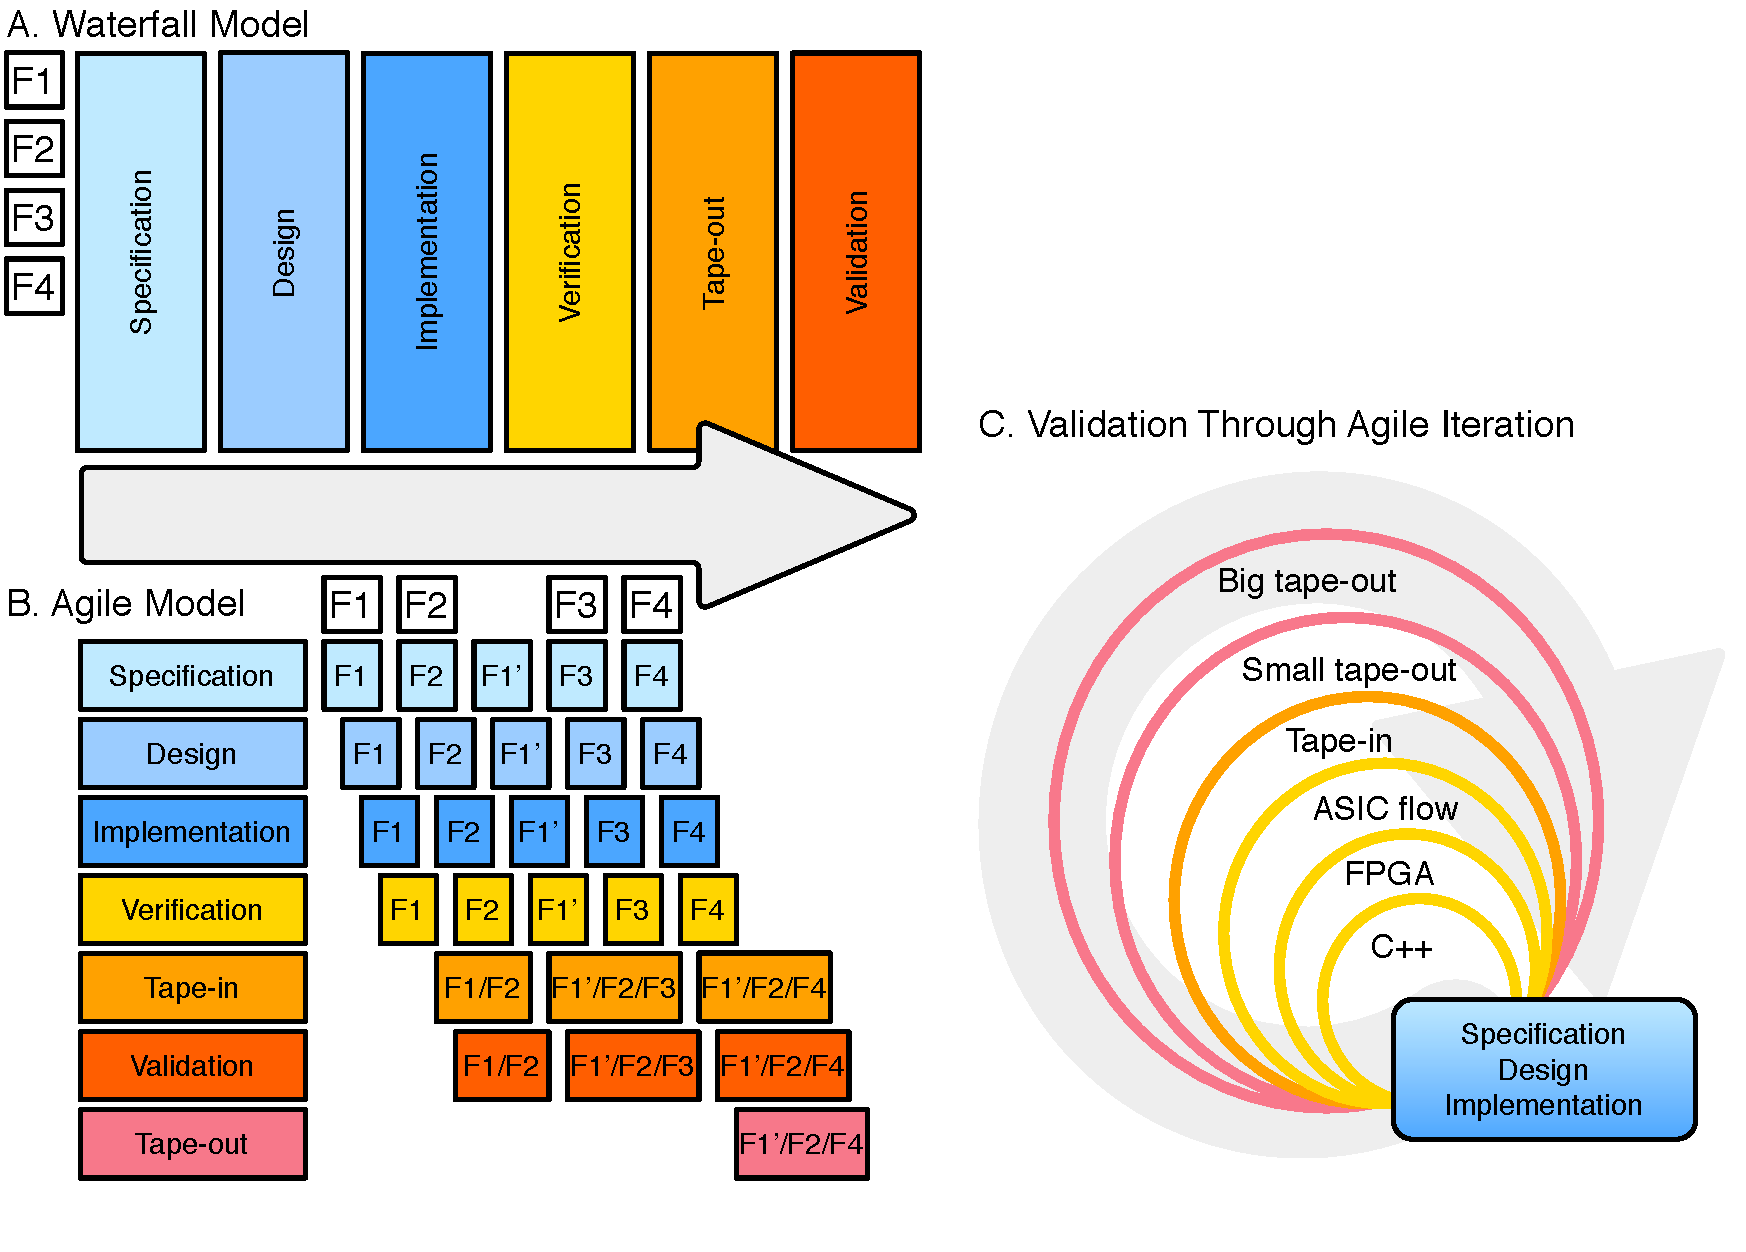
\includegraphics[width=1\columnwidth]{intro/figures/agile.pdf}
\caption{
Contrasting the agile and waterfall models of hardware design.  The labels F{\em N} represent various desired features of the design.
A. The waterfall model steps all features through each activity
sequentially, only producing a tapeout candidate once all features are complete.
B. The agile model adds features incrementally, resulting in incremental tapeout candidates as individual features are
completed, reworked, or abandoned.
C. As validation progresses, designs are subjected to lengthier and more accurate evaluation methodologies.
The circumfrence of each circle represents the relative time it takes to validate the design using a particular technology.
%Although the latency and cost of these prototype modeling efforts increases towards the outer circles, our confidence in the validation results produced increases in tandem.
}
\label{fig:agile}
\end{figure}

When applied in unison, these principles have substantially changed our developement model.
Figure~\ref{fig:agile} contrasts our agile development model with the waterfall model.
When applied to the hardware domain, the waterfall model encourages designers to rely on Gantt
charts, high-level architecture models, rigid processes such as RTL
freezes, and CPU-centuries of simulations in an attempt to achieve a
single viable design point (Figure~\ref{fig:agile}.A). 
In our agile hardware methodology, we first push a trivial prototype with a minimal working feature set all the way through the toolflow to a point where it could be taped out for fabrication.
We refer to this tape-out-ready design as a {\em tape-in}.
Then we begin adding features to it iteratively (Figure~\ref{fig:agile}.B).
After spec'ing out a particular feature and implementing it, 
we then deploy it against an increasing series of more complex tests on more heavyweight evaluation platforms, up to and including taping out prototype chips (Figure~\ref{fig:agile}.C).
Emphasizing a sequence of prototypes reduces verification simulation effort since early hardware prototypes run orders of magnitude faster than simulators. 

Conventional wisdom holds that the frequent deliverable prototypes required by agile methodology are incompatible with hardware development, but our research group has not found this to be the case \cite{lee-micro15}.
Firstly, using fabricatable prototypes increases validation
bandwidth, as a complete tape-in RTL design can be mapped to FPGAs to run
end-application software stacks orders of magnitude faster than with
software simulators. 
In agile hardware development, the FPGA models
of tape-in designs (together with accompanying QoR
numbers from the VLSI toolflow) fulfill the same function as working
prototypes do in agile software development, providing a way for
end-customers to give early and frequent feedback to validate design decisions.
Secondly, while mask costs for modern designs are on the order of multiples of millions of dollars depending on process technology \cite{sperling}, 
organizations like MOSIS continue to offer multi-project wafers, where many independent projects are put on the same reticle, to help amortize these mask costs.
As Moore's Law continues to slow down, industry will spend more time on each process technology node, leading to further reductions in the cost of doing multiple design iterations
%of increasingly complicated prototype test chips
at a given node.
%By reducing the minimal die size to around 1.5x1.5 mm we were able to bring the total cost of our prototype chips down to \$30,000, and 

Adopting the agile methodology dovetails nicely with our previously discussed tooling preference for building chip generators over particular chip design instances.
As we iteratively add features to the generator, we can retarget our efforts to adapt to performance and energy feedback from the previous iteration.
By parameterizing the design generator, we can smoothly scale the size of its output from test chip to final product without rewriting any hardware modules.
Note that we produced three distinct families of chips over four years in an interleaved fashion, {\em all from the same source code base}, but each specialized differently to try out distinct research ideas.
Figure~\ref{fig:tapeouts} presents the complete timeline of tapeouts that occurred using software components discussed in this thesis.
In particular, Chapter~\ref{c.parameters}'s focus on design parameterization techniques reflects the criticality of generator parameterization capabilities to our agile developement process.

As we will see, even a design choice as complicated and pervasive as a multi-level cache coherence protocol can be made a tuneable design parameter when properly factored out from the rest of the design.
By providing support for generating a family of compatible protocols rather than one single protocol, my thesis has enabled us to iterate on protocol design as we scaled up the size and complexity of the memory hierarchy across chip iterations.
%We were able to move from single-level, broadcast-based two-state protocol to a multi-level, hierarchical, directory-based, six-state protocol

\begin{figure}[t!]
\centering
\vspace{-0.15in}
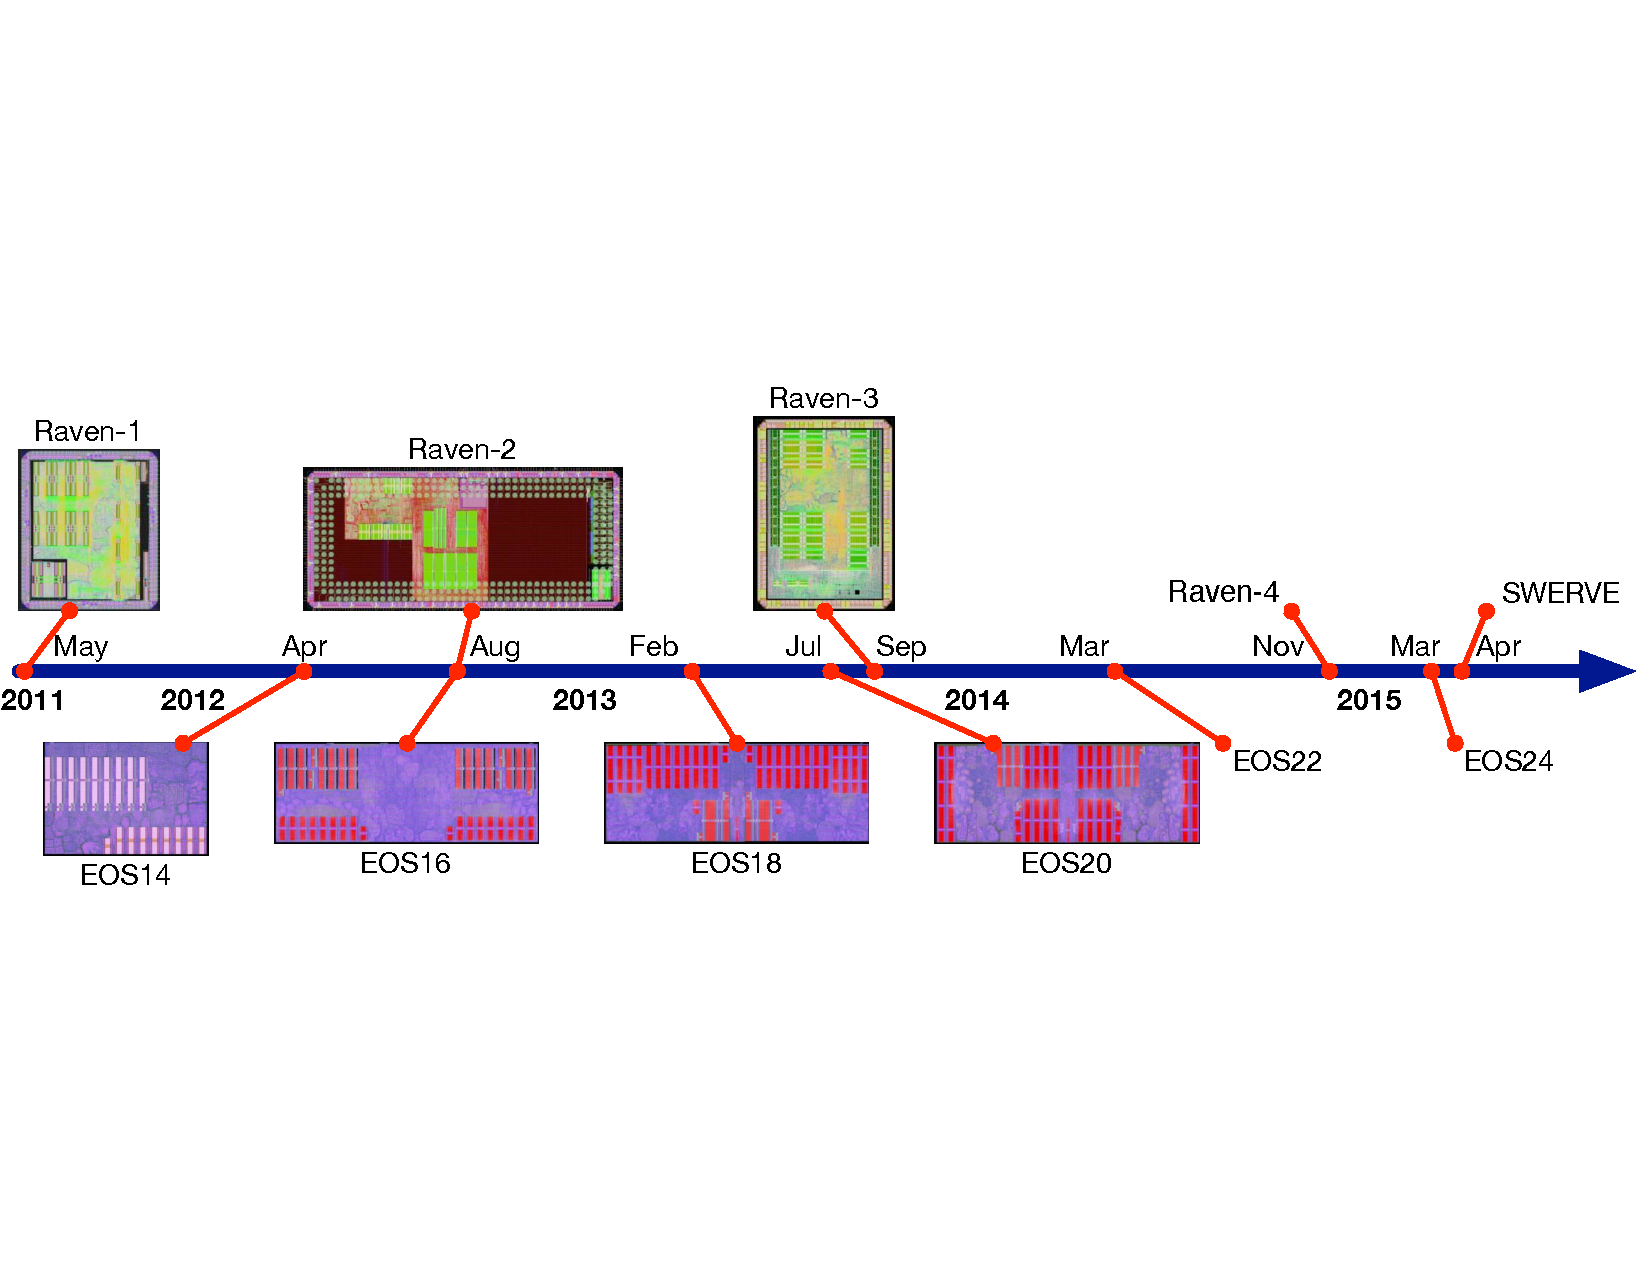
\includegraphics[width=\columnwidth]{intro/figures/tapeouts.pdf}
\vspace{-0.3in}
\caption{Lineage of UC Berkeley Chip Tape-Outs during the completion of my thesis.
The 28nm Raven chips combines a 64-bit RISC-V vector microprocessor with on-chip switched-capacitor DC-DC converters and adaptive clocking ~\cite{zimmer2015raven}.
The 45nm EOS chips integrate a 64-bit dual-core RISC-V vector processor with monolithically-integrated silicon photonic links ~\cite{lee2014eos}.
In total, we have taped out
four Raven chips on STMicroelectronics' 28nm FD-SOI process,
six EOS chips on IBM's 45nm SOI process,
and one SWERVE chip on TSMC's 28nm process. 
}
\label{fig:tapeouts}
\vspace{-0.1in}
\end{figure}

\subsection{Chisel}

To address the aforementioned language deficiencies and to enable more agile hardware design, together with my collaborators I have developed Chisel (Constructing Hardware In a Scala Embedded Language), a new hardware design language \cite{chisel}.
Chisel is a Domain-Specific Embedded Language (DSEL) that is built on top of the Scala programming language \cite{scala}.
Chisel is intended to be a substrate that provides a Scala abstraction of primitive hardware components, such as registers, muxes, and wires.
Any Scala program whose execution genereates a graph of such components is now a feasible way to fabricate hardware designs --- the Chisel compiler translates the graph into a backend language suitable for simulation or hardware synthesis.
For a particular design represented as a component graph, Chisel's backend can generate a fast, cycle-accurate C++ simulator, or generate structural Verilog suitable for either FPGA emulation or ASIC synthesis.

Because Chisel is embedded in Scala, hardware developers can now use Scala's modern programming language features to encapsulate many useful high-level hardware design patterns.
Designers may selectively deploy these patterns so as to generate graphs of Chisel components as productively as possible.
Each module in a Chisel project can employ whichever design patterns best fit the problem at hand, and designers can freely compose modules and programming paradigms as they build up more complicated designs.
Metaprogramming, code generation and hardware design tasks are all implemented in the same source language.
This single-source language approach encourages developers to write parameterized hardware generators rather than discrete instances of individual hardware blocks,
which in turn improves code reuse both within a given design and across generations of design iterations.
When combined with multiple backends catering to different stages of the verification process, the generator-based approach is essential to enable a more agile approach to hardware design.

Beyond implementing the Chisel compiler and releasing it as an open source software tool, my research group has worked to understand what types of hardware designs tasks can be encapsulated within resuable libraries that extend Chisel's functionality.
In some cases, these libraries have taken the form of discrete modules or parameterized functional units.
In other cases, the correct abstraction takes the form of a compiler pass, higher-order-functional API, or even a self-contained mini-DSEL.
Additionally, we have developed some pure Scala software utilities that aid in the hardware design process.
We have composed these various libraries of tools and generators into a complete SoC chip generator~\cite{rocket}.
In the next section I discuss the specific contributions my thesis makes to the Chisel ecosystem to aid in the design of cache coherent memory hierarchies.

\subsection{Rocket Chip Generator}

Chisel's first-class support for object-orientation and
metaprogramming allows hardware designers to write generators,
rather than individual instances of designs, which in turn encourages
the development of families of customizable designs.  By encoding
microarchitectural and domain knowledge
these generators, we can quickly create different
chip instances customized for particular design goals and constraints
\cite{shacham-micro10}.  As constructing hardware generators requires
support for reconfiguring individual components based on the context
in which they are deployed, a particular focus of Chisel is to improve
upon the limited module parameterization facilities of traditional
hardware description languages.

The Rocket chip generator is written in Chisel and constructs a
RISC-V-based platform.  The generator consists of a collection of
parameterized chip-building libraries that we can use to generate
different SoC variants.  By standardizing the interfaces that are used
to connect different libraries' generators to one another, we have
created a plug-and-play environment in which it is trivial to swap out
substantial components of the design simply by changing configuration
files, leaving the hardware source code untouched.  We can also both
test the output of individual generators as well as perform
integration tests on the whole design, where the tests are also
parameterized so as to exercise the entire design-under-test.

Figure~\ref{fig:generators} presents the collection of library generators and their interfaces within the Rocket chip generator.
These generators can be parameterized and composed into a wide variety of SoC designs.

\begin{figure}[t!]
\centering
\vspace{-0.3in}
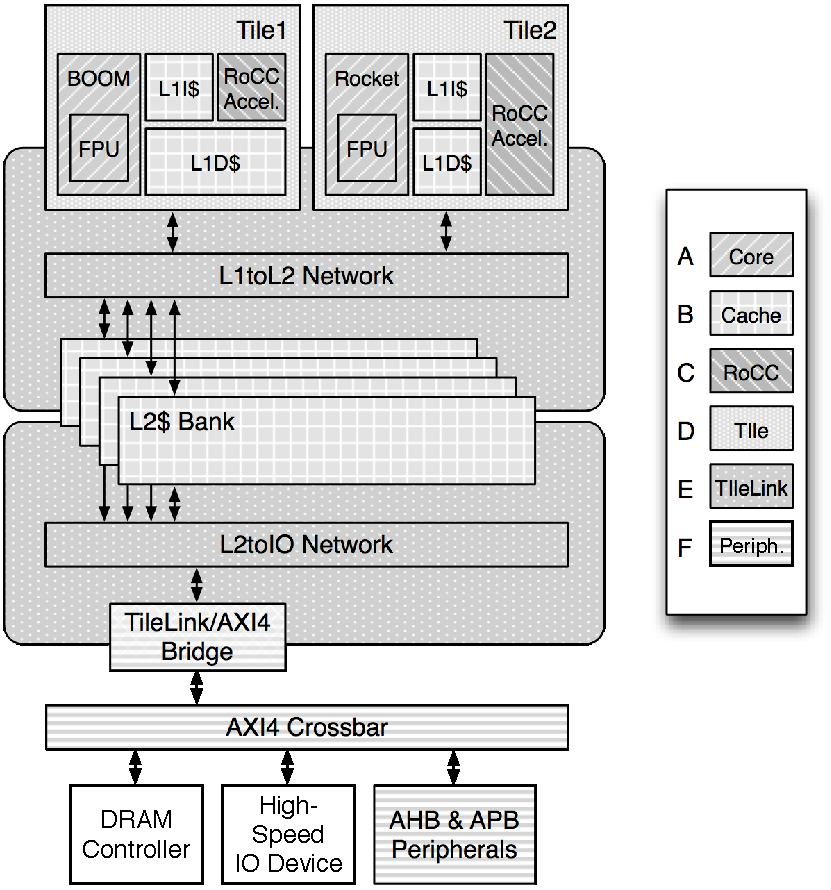
\includegraphics[width=.6\columnwidth]{intro/figures/rocket-chip.pdf}
\vspace{-0.15in}
\caption{The Rocket chip generator consists of the following sub-components: A) Core generator B) Cache generator C) RoCC-compatible coprocessor generator D) Tile generator E) TileLink generator F) Peripherals }
\label{fig:generators}
\vspace{-0.1in}
\end{figure}

\section{Contributions}

Given the increasing difficulty and ongoing importance of implementing efficient memory hierarchies and cache coherence protocols, it was natural to bring the productive power of Chisel to bear on these design problems.
My contributions focus on extending Chisel by providing libraries for hardware developers to use in describing the configuration and behavior of on-chip memory hierarchies, and particularly cache coherence protocols.
In this thesis I will make the case for how the abstractions I provide enable productive and composible memory hierarchy design.
My specific contributions are as follows:

\begin{enumerate}
\item A general framework for context-dependent parameterization of hardware modules.
\item A set of Chisel libraries for generating extensible cache-coherent memory hierarchies.
\item A methodology for decomposing high-level descriptions of cache coherence protocols into controller-localized transactions.
\end{enumerate}

\section{Collaborations}

This work would not have been possible without a variety of fruitful collaborations, and I would like to take the time to draw attention to certain individuals here.

Jonathan Bachrach, Huy Vo, and Andrew Waterman were my primary collaborators in developing the common utilities made available as part of the Chisel core distribution.
Jonathan's vision for what Chisel had the potential to become has been borne out in this thesis and all the chips taped out at Berkeley during my time here \cite{chisel}.
John Bachan and Adam Izraelevitz were instrumental in the developement of the context-dependent environment parameterization library,
which was initially published as a tech report \cite{cdeTR}.
Many other members of the Berkeley Architecture Research group also contributed to Chisel development and features. 

Andrew Waterman and Yunsup Lee entrusted me with the design and implementation of the memory hierarchy for multiple generations of the Raven and EOS lineages of test chips.
Working with them gave me a context and focus that forced me to search for both more productive abstractions and more efficient implementations,
and I also recognize the efforts of our other tape-out collaborators at the Berkeley Wireless Research Center and MIT.
Detailed discussions of our prototype chips were previously published
in~\cite{lee2014eos} and~\cite{zimmer2015raven},
while our proposal for an agile hardware development methodology was laid out in\cite{lee-micro15}.

\chapter{Context-Dependent Environments: \\ A Parameterization Paradigm for Hardware Generators}
\label{c.parameters}

As Moore's law fails, increasing demand for computational efficiency is no longer being matched by gains from process scaling. 
Instead, chip designers are improving efficiency by combining special-purpose accelerators with general-purpose processors in increasingly heterogeneous systems-on-chip.
In this new world of energy-efficient, heterogeneous, application-specific designs, it will be essential to both improve the productivity of hardware designers as well as enable extensive design-space exploration~\cite{shacham-micro10}.

Since it is not possible to build custom chips from scratch for every application,
we need hardware design tools that allow us to capture decisions made
during the process of designing one chip, yet easily make them differently when tackling a new target.
Creating parameterized hardware generators, rather than individual design instances, 
not only allows for application-specific customization of the final hardware,
it also gives designers the capability to preserve knowledge related to performance and energy trade-offs from previous design iterations.
By parameterizing aspects of the design, we can scale it from test chip sizes to final product without rewriting any modules, amortizing verification costs and increasing the validation confidence over time without rewriting code.
This templated, meta-programming approach is integral to our agile approach to hardware design.

The most salient feature of a hardware generator or template, as
compared to a single design instance, is that certain features of the design are
left under the control of the user deploying the generator within their chip.
We term these features the {\em parameters} of the generator.
{\em Parameterization} is the process by which a generator supplies values for each parameter,
i.e. binds the name of the parameter to a particular value,
before using that evaluation to elaborate details of the particular design instance at hand.
A {\em parameterization paradigm} codifies a particular way of expressing parameters and provides tools to support their application within generators,
as well as mechanisms to constrain their valuations.

The parameters and their constraints become the interface through which the generator author and the system architect communicate.
Constrained parameters serve as boundaries that define the space of designs which it is possible for the architect to explore.
By searching over the top-level parameters exposed by a set of such generators, System-on-Chip (SoC) chip architects can explore tradeoffs between performance, area, and energy efficiency.
By recording the outcomes of these explorations, these designers can build up a map of how to customize pieces of their design for a particular application's requirements.

Parameterization is clearly a first-order concern in the creation of tools based around specialized hardware generation.
In order to use generators productively, we need to understand how the choice of parameterization paradigm affects the design process.
We claim that the mechanism by which generator-based designs are parameterized can greatly influence three metrics of design robustness: reusability, composability, and modifiability.
We define these three metrics as follows:
\begin{description}
\item[Reusing] generators means that they can be instantiated as components of different broader hardware contexts with no internal source code changes, only differing parameterizations. Reusability amortizes verification overhead by reducing the number of lines of code used to create larger design instances.
\item[Composing] generators requires mechanisms to specify cross-generator parameter constraints and dependencies. Composability is mandatory to build up larger SoC designs consisting of multiple generators.
\item[Modifying] a generator (by adding a new parameters to it) should not cause a cascade of changes throughout any nested modules which instantiate that generator's output. Modifiability is predicated on \emph{modularity} in the code base, and mitigates technical debt that would encumber changing a generator's capabilities.
\end{description}

This chapter first provides a background discussion of how the concepts of parameterization and meta-programming are intertwined, as well as how software languages have addressed parameterization in the past.
We then provide a taxonomy of extant parameterization paradigms found in previous hardware description languages, and evaluate them in terms of the above metrics.
To correct for their deficiencies, we introduce \emph{context-dependent environments}~(CDEs), a new parameterization paradigm.
In the CDE paradigm, a key-value dictionary containing parameter bindings is passed through a hardware module hierarchy, and the value returned for each parameter identifier can depend on other parameter values at that query's origin within the design.
As we will see in this chapter,
the dynamic nature of a CDE's scoping, coupled with its context-specific knowledge, 
serves to support generator reusability and composition, while also improving a generator's robustness to any external module hierarchy modifications.

We provide both a case study and a formal analysis of design robustness with respect to each of the parameterization paradigms in our taxonomy, and prove that CDEs are the most robust option.
We then provide examples of how our open-source Scala implementation of CDEs is used in various sub-components of our RocketChip SoC generator.

As we will see later in this thesis, even a design choice as complicated and pervasive as a multi-level cache coherence protocol can be made a tunable design parameter when properly factored out from the rest of the design. 
By providing support for generating a family of protocols rather than one single protocol, my thesis has enabled us to iterate on protocol design as we scale up the size of the memory hierarchy across chip iterations.

\section{Background}
\label{sec:rel}

%Given a set of top-level configurations that supply value bindings for individual parameters, a generator can construct a vast number of different designs from a single piece of templated source code.
%Hardware generators are an increasingly popular paradigm; examples include Stanford's FPU generator~\cite{fpu}, Lawrence Berkeley National Lab's OpenSoC~\cite{opensoc}, and UC Berkeley's Rocket Chip Generator~\cite{rocket}.
%Bluespec provides AzureIP Libraries~\cite{azure} to give designers reusable components for use in custom generators. 
%Support for parameterization is a critical feature of the language in which the generator is written.

To provide context for our study of the applicability of various parameterization paradigms to hardware generation,
as well as to motivate the value of our new CDE paradigm,
we will first review two concepts at the heart of parameterization:
\emph{meta-programming} and \emph{name binding}.
Meta-programming allows us to create parameterized hardware templates, into which values can be injected to make concrete design instances.
Name binding is the process by which parameter identifiers are associated with particular values.

\subsection{Meta-programming}

When we talk about creating libraries of hardware generators instead of design instances,
the underlying concept that our design tools need to support is meta-programming of hardware descriptions.
A meta-program is a program that generates or manipulates program code~\cite{templates}.
Specifically in the case of this thesis, Chisel~\cite{chisel} is a meta-programming language (that is itself embedded in a host languagage, Scala).
Using Chisel, we can describe parameterized templates for particular hardware modules as Scala classes.
Executing a Scala program that instantiates particular instances of these classes allows the Chisel compiler
to elaborate a concrete design instance in Verilog or some other target language.
Because Chisel is embedded in Scala, we can use the full capabilities of this modern software language to implement our generators.
This chapter will make the case that one of the most essential capabilities that this embedding has put at our disposal
is the ability to use Scala to parameterize our hardware descriptions,
be it through built-in language capabilities or through parameterization frameworks written in the host language.

Traditional hardware description languages have lacked the language features to support parameterization of configurable designs.
Section \ref{sec:tax} will discuss how specific existing parameterization paradigms in Verilog, VHDL, SystemVerilog, and Bluespec SystemVerilog limit design modifiability and customizability.
However, because the outputs of our generators will be fully elaborated designs with parameter values  automatically embedded in them,
we can free generator authors from the constraints of the backend language with respect to choice of parameterization paradigm.
This approach also allows us to supply parameter bindings from external tools at hardware generation time,
which is a critical features for design space exploration~\cite{shacham2011chip}.
It is important to note that there are several different times during the hardware elaboration process where
we might decide to supply parameter values, and in particular, this chapter will discuss tradeoffs between
binding parameters to values at generator compile-time as opposed to generator run-time.

How parameters are expressed and referenced within and among generators is another important design question.
From the perspective of the author of a hardware generator, it is impossible to know the full context in which the components created by their generator will be instantiated.
The goal of the author of a hardware generator is to expose as many parameters as they possibly can to the user (e.g., an SoC architect)
while also recording any constraints the internals of the design put on those parameters' values.
Our parameterization paradigm must also accept constraints that are imposed by parent modules on their children, in the service of interoperability,
or by completely external tools, in the service of design space exploration.
Again, we are aided by the expressionality of the host language and the ability to connect with outside tools at hardware generation time.
Finally, while the parameters themselves are often merely instances of simple numeric or boolean types
depending on the nature of the meta-programming language,
we can also consider utilizing parameters that are bound to functions, user-defined objects, or other parameters.
As we will see, exploiting a host language's capability to use more complicated types in the parameterization framework
is an essential requirement for using it to support customizable cache coherence protocols.

Given the limitations of extant HDLs, adopting new ones with first class support for meta-programming (and thereby parameterization)
is critical to our hardware design methodology.
Chapter 3 of~\cite{shacham2011chip} provides additional discussion of the 
parameterization advantages related to meta-programming
in the context of Genesis2, a next-generation HDL embedded in Perl.
We include a comparison with Genesis2's Perl-based dynamic parameterization paradigm in Section \ref{sec:env}.

\subsection{Name Binding and Scoping}

The opportunity presented by embedding Chisel in Scala inspired us to examine parameterization solutions that have been investigated in software contexts.
Fundamentally, parameterization is a name binding problem, in which a data or code entity must be bound to an identifying name.
In our case, generators express the hardware they elaborate in terms of the parameters' identifiers,
while the framework is in charge of supplying the matching data as the hardware is generated.
What data is supplied for a particular name depends on the scoping of the identifier, which might be handled \emph{lexically} or \emph{dynamically}.
Lisp languages were the first to explore tradeoffs between dynamic scoping and lexical scoping \cite{gordon}.

With lexical scoping, in order to bind a name to an entity, we first search within the local function, then within the scope in which this function was defined, and so on.
``Lexical'' in this case refers to the text of the source code itself.
Lexical scoping provides referential transparency, which is a boon for both the programmer and compiler.
By analyzing the source code, it is possible to determine at compile time whether or not a particular binding is within scope.
Unfortunately, bindings needed by deeply nested components must be explicitly threaded throughout the class or function hierarchy.

With dynamic scoping, we again search first in the local function, but then search the function that called this function, and so on up the call stack of the running program.
``Dynamic'' in this case refers to the fact that the call stack can be different every time a given function is called, and so the binding created for the variable can thereby differ as well.
Dynamic binding is useful as a substitute for globally-scoped variables, and is excellent for deep customization of nested subsystems.
In cases where the necessary bindings may radically change from program instance to program instance, dynamic binding allows us to only specify those bindings that we know the current instance will use.
Unfortunately, in some cases programmer errors that could have been caught at compile time in a lexically-scoped system become runtime errors in a dynamically-scoped system.

While lexical binding is now the norm for most programming languages, many mechanisms have been developed to allow programmers to explicitly tie in dynamic binding benefits where they are useful.
These include special binding forms in most Lisp variants
(e.g., \code{fluid-let} in Scheme \cite{steele} and \code{parameterize} in Racket \cite{flatt2013racket}),
implicit parameters \cite{lewis2000implicit}, and the Reader monad in Haskell \cite{jones1995functional}.
While these approaches all focus on re-enabling the parameterization flexibility of dynamic binding in a more controlled manner, 
the context-dependent environments we propose here are actually a strictly more powerful mechanism than traditional dynamic binding. 
In general, taking advantage of later-binding solutions enables both more concise uniquification of elements of nested, heterogeneous systems~\cite{shacham2011chip},
and also allows us to deal with modifications to the hierarchy of generated modules more robustly.
The following taxonomy illustrates how selectively deploying our dynamic scoping solution is the best fit for hardware generation
by contrasting it with other lexically- and dynamically-scoped solutions.

\section{Taxonomy of Parameterization Paradigms}
\label{sec:tax}

Before introducing context-dependent environments, we first define and contrast three existing parameterization paradigms: argument lists, structs, and dynamic environments.
We examine how these paradigms could be or have been used in hardware description languages.
We then  evaluate them in terms of a simple case study
in which we describe making modifications to a hierarchical hardware generator that is composed from multiple sub-generators.
The three paradigms we contrast in this section are:

\begin{description}
\item[Argument Lists.] The default lexical binding approach wherein all parameters are explicitly passed to the constructor function of each hardware module class.
\item[Structs.] A more sophisticated lexical binding approach wherein user-defined datatypes are used to abstract away specific parameter binding sites.
\item[Environments.] A dynamic binding approach wherein an associative array of key-value pairs is used to supply parameter values at runtime.
\end{description}

We do not consider some other simple alternative parameterization solutions, such as a flat namespace of global constants, because such implementations lack composability and reuseability.
First, without a mechanism to manage namespace collisions between different third-party generators, composing generators without having to modify their internals becomes impossible.
Second, without a mechanism that allows designers to override parameter values within certain subsets of the module hierarchy, creating heterogeneous systems where the same generator
produces differently parameterized output becomes impossible.
For these reasons we only contrast the aforementioned three paradigms, as they support both design goals in their own ways.

%TODOEach scheme preserves module modularity and reusability by expressing all parameters at the top level and only requesting necessary parameters. We evaluate each paradigm's robustness by adding parameters/modules and counting the number of top-level (TLCs), non-local (NLCs), or local (LCs) source code changes cascading from this initial modification.

We can evaluate the robustness of these parameterization paradigms by adding new parameters or inserting additional modules, and then examining the source code changes required to bring the new parameter binding into scope. 
We differentiate three types of source code changes.

\begin{description}
\item[Local changes (LCs)] are the initial insertion or appending of a module instantiation with a new parameter. 
\item[Top-level changes (TLCs)] are new parameter bindings performed at the root of the module hierarchy. 
\item[Non-local changes (NLCs)] are any additional changes required to pass a top-level parameter value (bound by a TLC) to the scope of a lower-level module instantiation (created by an LC). 
\end{description}

LCs and TLCs are simply inherent to instantiating a new parameterized module or adding a new parameter to an existing module.
The module using the parameter must be instantiated somewhere in the hierarchy (LC), and the parameter must be bound to a value
somewhere in that instantiation's scope (TLC).
In some cases, additional LCs are needed to resolve conflicting parameter names at the location where the module is instantiated.

In contrast, NLCs only serve to bring a new parameter binding into scope for the new module instantiation,
or alternatively to correct an inter-module parameter reference that has been outdated by a module insertion.
We view being forced to manually make NLCs within our generators' source code as representative of
the brittleness of a particular parameterization paradigm in the face of changes to child generator interfaces
or module hierarchy depth.
In this way, NLCs are a form of technical debt imposed by the choice of parameterization framework on a hardware generator library.
According to our robustness metric, an ideal parameterization paradigm would eliminate all NLCs,
while simultaneously minimizing the number of LCs and TLCs needed to implement any given design modification.
In general, NLCs are the cost of deploying a paradigm dependent on lexical binding rather than dynamic binding.

%To maximize design modularity and reusability by first binding all parameter names at the top level of the module hierarchy and then requesting necessary parameter values within each module. 
%While default values could be supplied locally, any parameters used in inter-generator design space exploration must be exposed at the top level of each generator.

The following sections use examples written in Verilog-like pseudo-HDL code which elides non-parameter-related expressions.
Figure~\ref{fig:block} displays the block diagram organization of a set of nested hardware modules that we will use in our robustness case study.
We take a Tile generator that is hierarchically composed of Core, Cache, and FPU generators, and investigate how making modifications to the parameters
of the leaf generators impacts the rest of the design, as expressed in our pseudo-HDL.
Figure~\ref{fig:phdl} outlines the syntax for object declaration and instantiation in our pseudo-HDL.
In this pseudo-HDL, we assume every hardware module can be made into a templated hardware generator through the use of the additional \code{\#()} constructor parameter list.
Fields of that list (or fields of objects within the list) are the parameters of the generator/module in question.

\begin{figure}
\centering
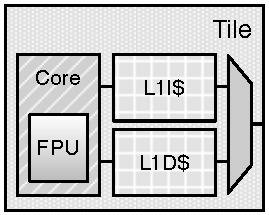
\epsfig{file=parameters/figures/tile.pdf, width=2.7in}
\caption[Organization of nested modules used in our running example.]{
Organization of nested modules used in our running example.
A Tile contains one Core and multiple Caches.
A Core may or may not contain an FPU, which may or may not be parameterized.}
\label{fig:block}
\end{figure}

\begin{figure}
\centering
\begin{phdl}
struct S {f:Bool,g:Int}          // struct declaration
module A #(p1,p2,p3,p4,p5)(...): ... 
   // module declaration: parameters use 1st argument list #(p1,...)
   // other RTL constructs like IOs use 2nd argument list (elided)
module B #()(...):
  a = new S(true, 1)             // struct instantiation
  b = a.f                        // struct access
  myA = new A #(a,b,c,d,e)(...)  // module instantiation
\end{phdl} 
\caption{Syntax for object declaration and instantiation in our HDL pseudocode.}
\label{fig:phdl}
\end{figure}

\subsection{Argument List Parameterization}

\begin{figure}
\centering
\begin{phdl}
module Top#()():
  hasFpu = true  // Whether our core should instantiate an FPU
  icSize = 64    // Size of the instruction cache's blocks
  dcSize = 64    // Size of the data cache's blocks
  myTile = new Tile #(hasFpu, icSize, dcSize)(...)
module Tile #(hasFpu, icSize, dcSize)(...):
  myCore = new Core  #(hasFpu)(...)
  icache = new Cache #(icSize)(...)
  dcache = new Cache #(dcSize)(...)
  assert (icSize == dcSize)         // The tile is multiplexing a single port
module Cache #(blockSize)(...): ... // icSize/dcSize each renamed blockSize
module Core #(hasFpu)(...):
  if(hasFpu) myFpu = new FPU()(...) ...
module FPU #()(...): ...
\end{phdl} 
\caption[An example module hierarchy.]{
An example module hierarchy containing a tile with a processor core and two caches, parameterized through constructor arguments.}
\label{fig:arglist}
\end{figure}

\begin{figure}
\centering
\begin{phdl}
module Top #()():
  hasFpu = true  // Whether our core should instantiate an FPU
  (*@\textcolor[rgb]{1,0,0}{fpuLat = 6}@*)     // Latency of FPU                               // TLC
  icSize = 64    // Size of the instruction cache's blocks
  dcSize = 64    // Size of the data cache's blocks
  myTile = new Tile #(hasFpu, icSize, dcSize,(*@\textcolor[rgb]{1,0,0}{fpuLat}@*))(...)        // NLC
module Tile #(hasFpu, icSize, dcSize,(*@\textcolor[rgb]{1,0,0}{fpuLat}@*))(...):               // NLC
  myCore = new Core  #(hasFpu, (*@\textcolor[rgb]{1,0,0}{fpuLat}@*))(...)                      // NLC
  icache = new Cache #(icSize)(...)
  dcache = new Cache #(dcSize)(...)
  assert (icSize == dcSize) 
module Cache #(blockSize)(...) : ... 
module Core #(hasFpu,(*@\textcolor[rgb]{1,0,0}{fpuLat}@*))(...) :                              // NLC
  if(hasFpu) myFpu = new (*@\textcolor[rgb]{1,0,0}{PFPU \#(fpuLat)}@*)(...) ...                 // LC
module PFPU #(latency)(...): ...     // Add parameter to FPU 
\end{phdl}
\caption[Modifying the example with argument lists.]{Example of the source changes (highlighted in red) that are required to append a new leaf submodule (PFPU) that contains a new parameter.}
\label{fig:arglist-delta}
\end{figure}

\emph{Argument list parameterization} is a paradigm wherein parameters are passed-by-value through class constructor function argument lists. 
It is the most basic, lexically-scoped way of binding parameters.
Verilog and VHDL are examples of existing HDLs that solely support this paradigm for parameterizing hardware modules.
 
Figure~\ref{fig:arglist} shows code describing the hierarchical \code{Tile} generator from Figure~\ref{fig:block} using argument list parameterization.
At the root of the module hierarchy, each parameter is bound to a value which is then passed into the module hierarchy via the argument list of \code{Tile}'s constructor.
These values are then propagated through the module hierarchy via the \code{Core} and \code{Cache} modules' constructors' argument lists.

In addition to injecting values into the design, we can enforce constraints on certain parameters.
For example, in this particular \code{Tile} architecture, both the instruction and data cache must have identical cache block sizes
because they are multiplexing the same memory port to the rest of the system.
This requirement is a property of this particular \code{Tile} generator; it was unknown to the designers of the \code{Cache} module.
Furthermore, other variations on a tile generator might not enforce this particular requirement, and so we would like to expose
\code{icSize} and \code{dcSize} to the design space explorer as independent, top-level variables.
Thus, the proper place to enforce the constraint is within \code{Tile}, making reference to the parameters that must be bound together.

Figure~\ref{fig:arglist-delta} illustrates how the argument list paradigm is brittle to modifications. 
We modify \code{Core} to use a parameterized FPU, \code{PFPU \#(fpuLatency)}, which takes as a parameter the desired latency for the unit.
In order to enact this modification, we must make several changes to the extant source code:
(1) a TLC to bind parameter \code{fpuLatency} in \code{Top};
(2) a LC to instantiate the new \code{PFPU} within \code{Core};
(3) four NLCs to \code{Tile} and \code{Core}'s declaration parameter lists, as well as \code{Tile} and \code{Core}'s instantiations.
The four NLCs represent the brittleness of this particular paradigm, in that adding a parameter to a leaf module causes many non-local changes to be required in any interstitial modules.
For small designs with simple class hierarchies, the total number of NLCs might be small.
However, as we will see in Section~\ref{sec:scca}, in this paradigm the number of NLCs scales with module hierarchy size, making modifications increasingly burdensome
as the collection of generators in a particular library grows.

Further complexity arises if we consider a set of different FPU implementations, each with a unique or even partially overlapping set of parameters.
The set of parameters included in each intervening module's constructor becomes the superset of all the child modules' parameters.
Determining which parameters are actually unique and supplying default values for any which are unused in a particular design instance becomes onerous
as more and more combinations of generators are composed.

\subsection{Struct Parameterizations}

\begin{figure}
\centering
\begin{phdl}
struct TilePars {hasFpu:Bool, icSize:Int, dcSize:Int} // Structs definitions
struct CorePars {hasFpu:Bool}
module Top #()():
  tp = new TilePars(true, 64, 64)                     // Struct instantiation
  myTile = new Tile #(tp)(...)
module Tile #(params)(...):
  cp = new CorePars(params.hasFpu)                    // Struct instantiation
  myCore = new Core  #(cp)(...)
  icache = new Cache #(params.icSize)(...)
  dcache = new Cache #(params.dcSize)(...)
  assert (params.icSize < params.dcSize)
module Cache #(blockSize)(...) : ...
module Core #(params)(...):
  if(params.hasFpu) myFpu = new FPU()(...) ...
module FPU #()(...): ...
\end{phdl} 
\caption[Parameterizing the example with flat structs.]{The same example module hierarchy, but parameterized through flat structs instead of argument lists.}
\label{fig:flatstruct}
\end{figure}

\begin{figure}
\centering
\begin{phdl}
struct TilePars {hasFpu:Bool, icSize:Int, dcSize:Int, (*@\textcolor[rgb]{1,0,0}{fpuLat:Int}@*)} // NLC
struct CorePars {hasFpu:Bool, (*@\textcolor[rgb]{1,0,0}{fpuLat:Int}@*)}                         // NLC
module Top #()():
  tp = new TilePars(true, 64, 64, (*@\textcolor[rgb]{1,0,0}{6}@*))                              // TLC
  myTile = new Tile #(tp)(...)                                    // No NLC
module Tile #(params)(...):                                       // No NLC
  cp = new CorePars(params.hasFpu, (*@\textcolor[rgb]{1,0,0}{params.fpuLat}@*))                 // NLC
  myCore = new Core  #(cp)(...)                                   // No NLC
  icache = new Cache #(params.icSize)(...)
  dcache = new Cache #(params.dcSize)(...)
  assert (params.icSize < params.dcSize) ...
module Cache #(size)(...) : ...
module Core #(params)(...) :                                     // No NLC
  if(params.hasFpu) myFpu = new (*@\textcolor[rgb]{1,0,0}{PFPU \#(params.fpuLat)}@*)(...) ...   // LC
module PFPU #(latency)(...): ...     // Add parameter to FPU 
\end{phdl} 
\caption[Modifying the example with flat structs.]{
Example of the source changes (highlighted in red) that are required to append a new leaf submodule (PFPU) that contains a new parameter,
under the flat-struct paradigm.}
\label{fig:flatstruct-delta}
\end{figure}

If the HDL provides user-defined struct types, these can be used to encapsulate multiple parameters within individual statically-typed objects.
SystemVerilog and Bluespec SystemVerilog are two HDLs that provide this capability.
For the purposes of our taxonomy, we posit that parameterization paradigms based on structs can be organized in two particular ways.
In \emph{flat-struct parameterization}, each generator is paired with a used-defined struct type containing all parameters used by that generator and all of its children.
This approach provides only a very limited advantage over the previously discussed argument list paradigm.
In \emph{nested-struct parameterization}, instead of a generator's companion struct consisting of a flat list of parameters,
it contains its own local parameters, as well as the parameter structs for its immediate children. 
This nesting allows further abstraction of the specific fields of the child generators' structs.

Both of these schemes are still lexically scoped, but we have moved the site of the bindings into a class hierarchy of struct types,
which may be distinct from the module hierarchy itself.
This level of indirection affords us, as generator authors, some opportunities to abstract away the specifics of what parameters are needed by which children.
By reducing the number of places we have to explicitly pass individual parameters' bindings from parent module to child module, we congruently reduce
the amount of work it takes to thread new parameters through the same module class hierarchy.
Encapsulation through structs can reduce the burden of lexical scoping in the face of design modifications.

Taking this idea a step further, we can recognize that we do not have to maintain a one-to-one mapping between the class hierarchy of structs and the class hierarchy of modules.
In the most extreme case, we could put all top-level parameters into a single struct which is passed to every module in the design,
essentially recreating a flat parameter paradigm based on global constants.
Such a solution improves modifiability by eliminating all NLCs but is problematic for composability,
because it means that sub-modules within the design cannot be reused in other contexts without providing default bindings for all possible parameters from all contexts.
However, more moderate solutions that exploit differences in the struct hierarchy and module hierarchy are possible at the designers' discretion.
For simplicity, the rest of this section utilizes the simpler one-to-one mapping to illustrate the differences between the struct paradigms.

Figure~\ref{fig:flatstruct} and Figure~\ref{fig:flatstruct-delta} show how the flat-struct paradigm,
applied with a one-to-one mapping between modules and structs,
can still eliminate some non-local changes in the face of appending the PFPU module as before.
This reduction happens because the module constructor argument lists do not grow with additional parameters.
While the definitions of all the structs must be changed to account for the new parameter,
instances where a single struct instance is passed to multiple module instantiations do not need to be changed,
because the module instantiation no longer references the individual parameters as they are now encapsulated fields of the struct.
However, Figure~\ref{fig:flatstruct-delta} shows that when inserting the newly parameterized \code{PFPU},
this scheme still requires some non-local changes because every parent generators's parameter struct declaration and instantiation must be changed.
In Section~\ref{sec:scca} we will see that the flat-struct paradigm is only a constant factor less brittle than the argument list paradigm.

\begin{figure}
\centering
\begin{phdl}
struct CorePars {hasFpu:Boolean, (*@\textcolor[rgb]{1,0,0}{fpuLat:Int}@*)}                     // NLC
struct TilePars {cp:CorePars, icSize:Int, dcSize:Int}            // No NLC
module Top #()():
  cp = new CorePars(true ,(*@\textcolor[rgb]{1,0,0}{fpuLat}@*))                                // TLC
  tp = new TilePars(cp, 64, 64)                                  // No NLC
  myTile = new Tile #(tp)(...)                                   // No NLC
module Tile #(params)(...):                                      // No NLC
  myCore = new Core  #(params.cp)(...)                                                        
  icache = new Cache #(params.icSize)(...)
  dcache = new Cache #(params.dcSize)(...)
  assert (params.icSize < params.dcSize) ...
module Cache #(size)(...): ...
module Core #(params)(...):                                     // No NLC
  if(params.hasFpu) myFpu = new (*@\textcolor[rgb]{1,0,0}{PFPU \#(params.fpuLat)}@*)(...) ...   // LC
module PFPU #(latency)(...): ...     // Add parameter to FPU 
\end{phdl} 
\caption[Modifying the example with nested structs.]{Example of the source changes (highlighted in red) that are required to append a new leaf submodule (PFPU) that contains a new parameter,
under the nested-struct paradigm.}
\label{fig:nestedstruct-append}
\end{figure}

\begin{figure}
\centering
\begin{phdl}
struct CorePars {hasFpu:Bool, fpuLat:Int}
struct TilePars {cp:CorePars, (*@\textcolor[rgb]{1,0,0}{cpf:CachePFPars}@*), dcSize:Int}      // NLC
struct CachePfPars {dist: Int, size:Int} // New struct for Prefetcher
module Top #()():
  (*@\textcolor[rgb]{1,0,0}{cpf = new CachePfPars(16, 64)}@*)  // Icache size now nested      // TLC
  cp = new CorePars(true, 6)
  tp = new TilePars(cp, (*@\textcolor[rgb]{1,0,0}{cpf}@*), 64)                                // NLC
  myTile = new Tile #(tp)(...)
module Tile #(params)(...):
  myCore = new Core  #(params.cp)(...)
  icache = new (*@\textcolor[rgb]{1,0,0}{CacheWithPF \#(params.cpf)(...)}@*)                   // LC
  dcache = new Cache #(params.dcSize)(...)
  assert ((*@\textcolor[rgb]{1,0,0}{params.cpf.size}@*) < params.dcSize)                      // NLC
module CacheWithPF #(params)(...):  // New module that adds prefetch functionality to cache
  myCache = new Cache #(params.size)(...)
... // Cache, Core, FPU declarations are unchanged
\end{phdl} 
\caption[Inserting a new module with nested structs.]{
Example of the source changes (highlighted in red) that are required to insert a new interstitial submodule (CacheWithPF) that contains a new parameter,
under the nested-struct paradigm.}
\label{fig:nestedstruct-insert}
\end{figure}

We can instead adopt \emph{nested-struct parameterization} to avoid the aforementioned cascading changes to all parent parameter structs' declarations and instantiations. 
Instead of a generator's companion struct consisting of a flat list of parameters, it contains only its own locally-consumed parameters as well as the parameter structs for its immediate children. 
Figure~\ref{fig:nestedstruct-append} applies this approach to the previous example of appending a parameterized FPU.
Only \code{PFPU}'s immediate parent's companion struct, \code{CorePars}, needs modification.
The fact that \code{CorePars} now has an additional parameter associated with it is now abstracted away from both \code{Tile} and \code{TilePars}.

Although the nested-structs paradigm eliminates almost all NLCs related to {\em appending} new leaf modules to the hierarchy,
it retains another disadvantage related to {\em inserting} new levels into the module hierarchy.
Figure~\ref{fig:nestedstruct-insert} provides an example of a such a scenario.
Suppose we want to add a prefetcher to our instruction cache. 
We insert module \code{CacheWithPF}, with a single parameter (\code{distance}), that instantiates our original \code{Cache} module inside of itself.
\code{CacheWithPF} wraps \code{Cache}'s output with additional logic to perform prefetching of expected instructions up to a specified \code{distance}.

The nested-struct paradigm does allow us to add \code{distance} without changing \code{Tile}'s constructor, avoiding an NLC.
Unfortunately, adding a new level of nesting in the parameter structs breaks our previously-existing assert statement in \code{Tile}. 
Because the nested structure of the parameter objects explicitly mirrors the generator hierarchy,
any changes to the nesting will break references to any child's parameters on which parent generators are enforcing constraints.
This restriction results in a whole new class of NLCs to deal with, ones that could never have arisen with the simpler argument list approach!

While both struct paradigms are acceptable for flat class hierarchies with limited possible nestings,
generators often have deep module hierarchies or interoperate with other generators from multiple libraries
(correct interoperation often necessitates the imposition of constraints in parent generators).
These lexically-scoped paradigms embrittle such designs because changes to the module hierarchy break a parent's references to its childrens' parameters. 
Note that these broken references can be located anywhere in the design
and are often not located near the LC that inserts the new module.
Overall, even nested-structs cannot guarantee a robust design, despite significantly reducing NLCs related to appending new leaf modules.
Unsatisfied with lexical scoping for deeply nested generator hierarchies, we now turn our attention to dynamic scoping solutions.

\subsection{Environment Parameterization}
\label{sec:env}

We begin by characterizing an environment-based approach to dynamic scoping of parameters.
An \emph{environment} is an associative array (i.e., map, dictionary), where each key and value pair consists of a parameter identifier and value respectively.
Environments can be inherited by an instance of a module and then passed along to its children, possibly
with modifications made to the key-value bindings.
Code within modules can gain access to certain parameter values by looking up the parameter's key in the environment.

Environments are a dynamic scoping solution because the value returned for each key is determined based on the execution of the program,
not the hierarchy of the source classes.
As alluded to earlier in this chapter, there are some tradeoffs inherent to dynamism.
Critically for composability, we do not have to pass bindings for all possible parameters through the module hierarchy explicitly.
This flexibility is a great boon for generators where some parameters are only used if certain other parameters are set a particular way,
or in cases where homogenous designs may be uniqueified to form heterogeneous ones.
If a particular instance of a design does not use a particular parameter, that parameter never has to be bound.
If a new module is added, bindings for its parameters can be supplied to the environment from any parent location in the hierarchy.
The cost we pay for this flexibility is that unbound parameters can only be detected at runtime, rather than at compile time.

A popular use of dynamic environments in the software world are those used for processes in all flavors of Unix.
Whereas shell languages in Unix systems have a first-class syntax for accessing environment values (e.g. \code{\$HOME}),
attempts to implement environments in a previously existing HDL would have to explicitly pass the environment object through the module hierarchy to query it.
Unfortunately, SystemVerilog and BluespecSV (as well as Verilog and VHDL) cannot support environments, as environments require either nested functions or HashMaps.
While the SystemVerilog language includes associative arrays (similar to HashMaps), most SystemVerilog compilers do not support it.
This type of environment could be implemented in Bluespec or SystemVerilog using tagged unions or associative arrays.
Unfortunately, neither language supports dynamically typed parameters, and thus cannot pass associative arrays as parameter objects.
Bluespec requires that all type checking be resolved prior to elaboration; since the compiler cannot guarantee that the returned value is type safe, associative arrays are not supported. 
Tagged unions, however, can be statically-type safe and used if the types of all parameters are known.
While both BluespecSV and SystemVerilog claim support for tagged unions, many SystemVerilog compilers lack support for them.

Chisel and Genesis2 leverage Scala and Perl, respectively, for metaprogramming the module hierarchy generation stage of hardware elaboration.
Because Scala and Perl support first-class functions and maps, both HDLs can easily provide the type of environment discussed here using either.
As we will see in Section~\ref{sec:impl}, Scala's support for implicit parameters makes it syntactically concise to distribute
the environment object through the module hierarchy.
Perl allows the programmer to select whether a variable is a dynamic global variable or a lexically-scoped local variable.
Rather than depend on the functionality global Perl environment, Genesis2 defines its own parameter environment framework that provides additional features.

Genesis2 supplies a parameter environment for each module and provides an API that allows users to:
define parameters,
assign them default values,
override those values from external configuration files,
force parameters to always take certain values,
and
define additional parameters at module instantiation time
\cite{shacham2011chip}.
A module can use a reference to any other module to make a reference to that module's parameters' values. 
Parameters are read-only, and queries return deep copies of mutable objects.
Because Perl is a dynamically-typed language, no type checking can be done on the return type of parameter queries.
The framework outputs XML to encapsulate the full ``configuration'', i.e., the text description of how SystemVerilog module declarations are composed.
This organization allows for iterative customization of certain parameters values within the design in accordance with the experimental design of external tools.
%Would need to explicitly rename parameters, can do this in multiple ways, including defining synonyms or referencing a parent's parameter. Adding parameters does require explicit renaming, no mechanism to reference child. Adding cde's would only benefit it, I think.

\begin{figure}
\centering
\begin{phdl}
x = {'key1' -> 1,'key2' -> 3} // Environment instantiation
y = x ++ {'key1' -> 2}        // Environment modification
print x('key1')               // Environment query, prints '1'
print y('key1')               // Environment query, prints '2'
print y('key2')               // Environment query, prints '3'
\end{phdl}
\caption{Syntax for environment instantiation, modification and querying in our pseudo-HDL.}
\label{fig:env-phdl}
\end{figure}

\begin{figure}
\centering
\begin{phdl}
module Top #()():
  topPars = {'hasFpu'->true, 'icSize'->64, 'dcSize'->64} // Top-level bindings
  myTile = #(topPars)(...)
module Tile #(params)(...):
  myCore = new Core  #(params)(...)
  icache = Cache #(params('icSize'))(...)          // Parameter lookup
  dcache = Cache #(params('dcSize'))(...)          // Parameter lookup
  assert (params('icSize') < params('dcSize')) ... // Parameter lookups
module Cache #(size)(...) : ...
module Core  #(params)(...) :
  if(params('hasFpu') myFPU = new FPU #()(...) ... // Parameter lookup
\end{phdl} 
\caption[Parameterizing the example through dynamic environments.]{
The same example module hierarchy, but parameterized through dynamic environments.}
\label{fig:env}
\end{figure}

\begin{figure}
\centering
\begin{phdl}
module Top #()():
  topPars = {'hasFpu' -> true, 'icSize' -> 64, 'dcSize' -> 64, (*@\textcolor[rgb]{0,0,1}{'fpuLat' -> 6}@*), (*@\textcolor[rgb]{1,0,0}{'dist' -> 16}@*) } // TLCs
  myTile = Tile #(topPars)(...)                                  // No NLC
module Tile #(params)(...):                                      // No NLC
  myCore = Core #(params)(...)                                   // No NLC
  // The following rename from `icSize' to `size' must be handled here by icache's parent
  (*@\textcolor[rgb]{1,0,0}{icPars = params ++ \{'size' -> params(`icSize')\}}@*)                // LC for CacheWithPF
  icache = new (*@\textcolor[rgb]{1,0,0}{CacheWithPF \#(icPars)(...)}@*)                        // LC for CacheWithPF
  dcache = new Cache #(params('dcSize'))(...)
  assert (params('icSize') < params('dcSize')) ...
module CacheWithPF #(params)(...) :
  Cache #(params('size'))(...) ... // CacheWithPF queries 'size'
module Core #(params)(...) :
   if(params('hasFpu') myFPU = new (*@\textcolor[rgb]{0,0,1}{PFPU \#(params('fpuLat'))}@*)(...) // LC for PFPU
... // Cache, PFPU module declarations are unchanged
\end{phdl} 
\caption[Modifying the example with dynamic environments.]{
Simultaneously appending a new submodule that contains a new parameter (highlighted in blue), while also inserting
a new interstitial module that contains a new parameter (highlighted in red). Dynamic environments eliminate NLCs.}
\label{fig:env-delta}
\end{figure}
Figure~\ref{fig:env-phdl} provides an overview of the additional syntax we introduce to our pseudo-HDL in order to allow it to support instantiation, modification, and querying of environments.
An important note is that the \code{++} operator, which adds a binding to the store, returns a new environment and does not affect the original environment.
In addition, all values in key-value pairs are lazily evaluated only when a query matches on a particular key.

Figure~\ref{fig:env} shows the code for our running example of the tile generator, modified to use the environment to supply parameters to all modules with two or more parameters.
To parameterize a child module, a parent copies its own environment and adds/overwrites any needed key-value mappings before passing it to the child.
While keys can be overridden in certain sub-modules, the overall namespace provided by the environment is flat and does not codify anything about the structure of the module hierarchy.
Figure~\ref{fig:env-delta} demonstrates the advantages of this flexiblity by applying both of the modifications from previous case study examples
(replacing the appended \code{FPU} with \code{PFPU} and inserting \code{CacheWithPF}).
Significantly, the only changes required are LCs and TLCs, with no NLCs whatsoever.
Even the cross-module assertion on cache sizes in \code{Tile} does not require modification.

Although the environment passing paradigm succeeds in removing all NLCs,
there is an additional LC required to rename the \code{icSize} parameter to \code{size}.
Why does \code{CacheWithPF} query for \code{size} instead of \code{icSize}?
The generator designer engineered it to be composable with any cache, and to avoid binding it to a particular instance.
We should not contextualize the parameter name (e.g., change \code{size} to \code{icSize}),
because in a different design the sub-module that is instantiated could be a data cache. 
Thus, an explicit renaming step is necessary to customize the parameter environment passed to \code{CacheWithPF}, telling it which top-level parameter to use
in response to any internal queries made regarding \code{size}.
We consider the source code change, required to perform the renaming by modifying the environment, an LC rather than an NLC, because it always occurs in conjunction
with the LC that instantiates the newly inserted module.
However, it is worth noting that the renaming must be performed for each unique instance of the module that takes on a different, heterogeneous value.

In general, we will often have modules that have either intentionally picked a context-free key or have simply used parameter keys that coincidentally overlap with those
used by some other imported generator.
Differentiating these conflicting keys and assigning them to the proper top-level key bindings is both the power and the burden of the dynamic environment paradigm.
For designs that do not have a large number of parameter key collisions, environment passing is a great solution as it will significantly reduce the number of NLCs. 
Unfortunately, in the prevalent case of designs that have many instances of the same child module class (e.g., a mesh of routers), the re-mapping of unique top-level parameters onto generic, re-used child parameters,
that must occur every time one of these children is instantiated, becomes onerous.
To mitigate this burden through the use of geographic information, we now turn to context-dependent environments.

\section{Context-Dependent Environments}
\label{sec:cde}

\begin{figure}
\centering
\begin{phdl}
module Example :
  env1 = {'whoami' -> (*@\textcolor[rgb]{1,0.5,0}{\textbf{\textit{site}}}@*)('coord')}                // CDE instantiation
  env2 = env1 ++ {'coord' -> 'environment 2'} // CDE modification
  print env1('whoami')                        // CDE query, prints 'Error: 'coord' is not defined'
  print env2('whoami')                        // CDE query, prints 'environment 2'
\end{phdl}
\caption{Syntax for CDE instantiation and querying in our pseudo-HDL.}
\label{fig:cde-phdl}
\end{figure}

\begin{figure}
\centering
\begin{phdl}
module Top #()():
  constPars = { 'coefficient' -> 4 }                               // Constant function
  indexPars = { 'coefficient' -> List(4,5,6,7).at((*@\textcolor[rgb]{1,0.5,0}{\textbf{\textit{site}}}@*)('index')) } // Function on 'index'
  myHomogenousDSP   = new DSP4MultArray(constPars)     // Makes a DSP with identical coefficients
  myHeterogenousDSP = new DSP4MultArray(indexPars)     // Makes a DSP with unique coefficients
module DSP4MultArray #(params)(...):
  mult0 = new Mult #(params ++ {'index' -> 0}) m0(...) // DSP4MultArray provides context
  mult1 = new Mult #(params ++ {'index' -> 1}) m1(...)
  mult2 = new Mult #(params ++ {'index' -> 2}) m2(...)
  mult3 = new Mult #(params ++ {'index' -> 3}) m3(...) ...
module Mult #(params)(...):
  c = params('coefficient') ...                        // Mult only knows about coefficient, not index
\end{phdl}
\caption{Example of specifying geographic information using site in pseudo-HDL.}
\label{fig:site-phdl}
\end{figure}

We now describe the functionality of our novel context-dependent environments paradigm for parameterization
and assess its robustness using the case study introduced in the previous section.
In the CDE paradigm, we again pass an associative array called an environment through a hardware module hierarchy, but the environment itself has an additional capability:
the value returned for a query on a key can depend on other parameter values at that query's origin within the design.
This feature is deceptively simple; the level of additional indirection provided in a CDE is a powerful tool for describing
parameters in terms of one another, which aids us in cascading uniquifying changes through subsets of a heterogeneous design.

While we previously demonstrated how we can use environments to provide the flexibility of dynamic binding on-demand from within a lexically-scoped module hierarchy, 
the CDEs we propose here are actually a strictly more powerful mechanism than traditional dynamic binding. 
We owe this power boost to our decoupling of ``how'' and ``when'' to compute a parameter's value,
allowing the ``how'' to be specified at binding time,
but deferring evaluation until the time at which the parameter is actually queried during elaboration.
This ``lazy'' evaluation strategy permits more parameter bindings to be in scope at
evaluation time than were available at binding time,
with the advantage that these other parameters may come from code locations not visible to the original binding site.

Mechanically, the sole additional feature of a CDE over a regular environment is a special object, called \emph{site}, that dynamically points to the originating CDE of the parameter query.
\emph{site} is available to be queried when defining the value bound to a particular identifier.
In other words, environment values bound within the environment are no longer mere literals, instead
they have been promoted to functions that take as an argument a dictionary representing the view of the world as seen from the query's point of origin.
When the environment is asked to evaluate a particular parameter identifier, the function stored for that key in the dictionary is evaluated against the dictionary itself.
Regular style environment variables are still possible in this paradigm, but now are just functions that ignore the dictionary argument and return a constant value (i.e. constant functions). 
We call these enhanced environments {\em context-dependent} because the valuations taken by their bindings depend on where the query is made.

\begin{figure}[p]
\centering
\begin{phdl}
module Top #()() :
  topPars = {'hasFpu' -> true,
             'size' -> if((*@\textcolor[rgb]{1,0.5,0}{\textbf{\textit{site}}}@*)('loc') == 'iCache') 64 else 64 }
  myTile = new Tile #(topPars)(...)
module Tile #(params)(...):
  myCore = new Core #(params)(...)
  icache = new Cache #(params ++ {'loc' -> 'iCache'})(...) // Insert geographic location
  dcache = new Cache #(params ++ {'loc' -> 'dCache'})(...) // Insert geographic location
  assert (icPar('size') < dcPar('size')) ...
module Cache #(params)(...):
  ... params('size') ... // Cache queries CDE directly
module Core #(params)(...):
  if(params('hasFpu') myFpu = new FPU()(...) ...
\end{phdl} 
\caption[Parameterizing the example with CDEs.]{The same example module hierarchy, but parameterized through context-dependent environments.}
\label{fig:cde}
\end{figure}

\begin{figure}
\centering
\begin{phdl}
module Top :
  topPars = {'hasFpu' -> true,
             (*@\textcolor[rgb]{1,0,0}{'dist' -> 16}@*),                                   // TLC
             (*@\textcolor[rgb]{0,0,1}{'fpuLat' -> 6}@*),                                  // TLC
             'size' -> if((*@\textcolor[rgb]{1,0.5,0}{\textbf{\textit{site}}}@*)('loc') == 'iCache') 64 else 64 }
  myTile = new Tile #(topPars)(...)
module Tile (params)(...):
  myCore = new Core #(params)(...)
  icache = new (*@\textcolor[rgb]{1,0,0}{CacheWithPF}@*) #(params ++ {'loc' -> 'iCache'})(...) // LC
  dcache = new Cache #(params ++ {'loc' -> 'dCache'})(...)
  assert (icPar('size') < dcPar('size')) ...
module Cache #(params)(...):
  ... params('size') ...
module CacheWithPF (params)(...):
  Cache #(params)(...)        // CacheWithPF simply passes CDE
module Core (params)(...) :
  if(params('hasFpu') myFpu = new (*@\textcolor[rgb]{0,0,1}{PFPU \#(params)}@*)(...) // Core simply passes CDE  // LC
\end{phdl} 
\caption[Modifying the example with CDEs.]{Simultaneously appending a new submodule that contains a new parameter (highlighted in red), while also inserting
a new interstitial module that contains a new parameter (highlighted in blue). Dynamic environments eliminate NLCs.}
\label{fig:cde-delta}
\end{figure}

Figure~\ref{fig:cde-phdl} provides a basic example of syntax and behavior for using the CDE {\em site} functionality in our pseudo-HDL.
We can see that \code{env1} is queried with the key \code{'whoami'}. 
This key is contained within \code{env1}, and its value, \code{site('coord')}, is evaluated. 
Because the original queried object is \code{env1}, \code{site} points to \code{env1} (i.e. \code{site('coord') == env1('coord')}). 
Since \code{env1} does not contain the key \code{'coord'}, this query fails.
The second query, \code{env2('whoami')}, matches because \code{env2} contains a \code{'whoami'} key. 
When \code{'whoami'}'s value is evaluated, \code{site('coord')} now points to \code{env2} (i.e. \code{site('coord') == env2('coord')}). 
Because \code{env2} contains a \code{'coord'} key, \code{site(`coord')} returns \code{'environment 2'}. 
This return value is propagated back to the original \code{env2('whoami')} callee and printed.

Now that every value in the environment can actually be a function of the bindings in the environment that is evaluating it, we can trivially
build meta-parameters that are based on formulae consisting of existing parameters, e.g. \code{\{"area"~->~site("length")~*~site("width")\}}.
This feature is a powerful capability for forming chains of parameter dependencies, in which parameters can be derived from other parameters.
Most importantly, these valuations can include reference to other parameters' keys which were not known to the original generator authors,
but which are instead being defined by other generators in the hierarchy.
For example, while the original author of the \code{"area"} key may have specified only that it returns an integer,
composition with a Circle generator would override it to be bound to \code{\{"area"~->~pi~*~site("radius")~*~site("radius")\}}, whereas
composition with a Square generator would override it to be bound to the above example.
Furthermore, the actual bindings for \code{"width"}, \code{"length"}, or \code{"radius"} do not have to be supplied at the same time that
the meta-parameter \code{"area"} is bound to its value function.
As long as any interstitial generator binds those keys before the generator that uses \code{"area"} actually evaluates its query on that key,
everything will dynamically resolve to the correct value.

This \emph{site} functionality is particularly useful in the context of hardware generation because 
it allows for specialization of parameter values based on contextual or ``geographic'' information that was injected into the environment by any intermediate generator in the module hierarchy.
This capability is at the heart of how we uniquify certain modules in a heterogeneous design.
Exploiting this capability requires that modules in a generator library built around the CDE paradigm follow the practice of placing geographic information
as new parameters in the environments they produce for their child modules, at the point where such geographic distinctions are clear. 
For instance, a network generator will instantiate and wire together the output of many router generators.
We would like a convenient way to assign different parameter values to the routers based on their location in the topology.
To achieve this effect, we place the burden on the parent generator (network) to append each child (router)'s inherited CDE with a constant parameter, e.g. \code{\{"location"~->~(x, y)\}}.
Assuming this geographic information will be dynamically inserted into the environment by the parent,
the top-level environment is free to tune each router's behavior according to \code{"location"}
by referencing it in the site-based function \code{\{"route"~->~if(site("location")~==~(1, 2))~...~\}}.
In a homogeneous system, \code{"route"} will be bound to a constant value.
In a heterogeneous system, we will supply whatever function we please on \code{"location"}
such that the individual locations will elaborate different designs.

Figure~\ref{fig:site-phdl} provides a more detailed example of geographic specialization.
We present an array of multipliers that use a parameterized coefficient, such as might be found in a DSP engine or FIR filter.
The structure of the design is fixed: \code{DSP4MultArray} has four multipliers.
However, we want to leave the binding of particular coefficients to particular multipliers up to the top level.
If we want a homogeneous set of multipliers, we can make the \code{'coefficient'} parameter a constant function.
If we want a heterogeneous set of multipliers, we can make the \code{'coefficient'} parameter a function of \code{'index'}.
The top-level parameter assignment may dispatch different values to the same query by using the geographic information known only at the origin of the query. 
In this case, \code{Mult} need know nothing about \code{'index'}.
Furthermore, we can use \code{'index'} in the top-level environment even though no generator has yet injected that key into the environment.
When we finally query \code{'coefficient'} inside of \code{Mult}, \code{site} resolves to an environment where the \code{'index'} key has since been defined (in the heterogeneous case).
This example demonstrates how components in a generator library built around CDEs can leave a hook (e.g. \code{index}) by which external modules can specialize them,
and shows how this capability is based on decoupling ``how'' and ``when'' to compute a parameter's value. 

While the context-dependent specialization provided by CDEs is a useful property for expressing heterogeneous hardware,
CDEs also improve on regular environments in terms of the robustness they provide in the face of module hierarchy modifications.
We return to the tile generator example from the previous section in Figure~\ref{fig:cde}, but now deploy the CDE \code{topPars}.
Note that, in this example, we show how we could use
\code{site} to specialize queries on \code{'size'} in order to uniquify the block size for each cache,
even though this particular tile generator requires them both to dynamically be set to have the same block size.

In Figure~\ref{fig:cde-delta} we now apply both modifications from Section~\ref{sec:tax} (i.e. replacing \code{FPU} with \code{PFPU} and inserting \code{CacheWithPF}).
Under the CDE paradigm, these modifications require only two TLCs and two LCs.
As before, using environments for dynamic binding eliminates the constructor-related NLCs and broken cross-module parameter references.
Furthermore, using \code{site} to specialize the cache line sizes means that we do not have to explicitly rename the \code{'size'} paramter, as we had to do for regular environments.
Changes to parameter bindings are handled through site-based indirections instead of in-line renamings.
This example supplies us with some intuition that the CDE paradigm is qualitatively superior to all previous paradigms.
It has fewer LCs and fewer NLCs, with an equivalent number of TLCs.
We formalize this qualitative assessment in the following section.

\section{Source Code Change Analysis}
\label{sec:scca}

\begin{figure}[p]
\centering
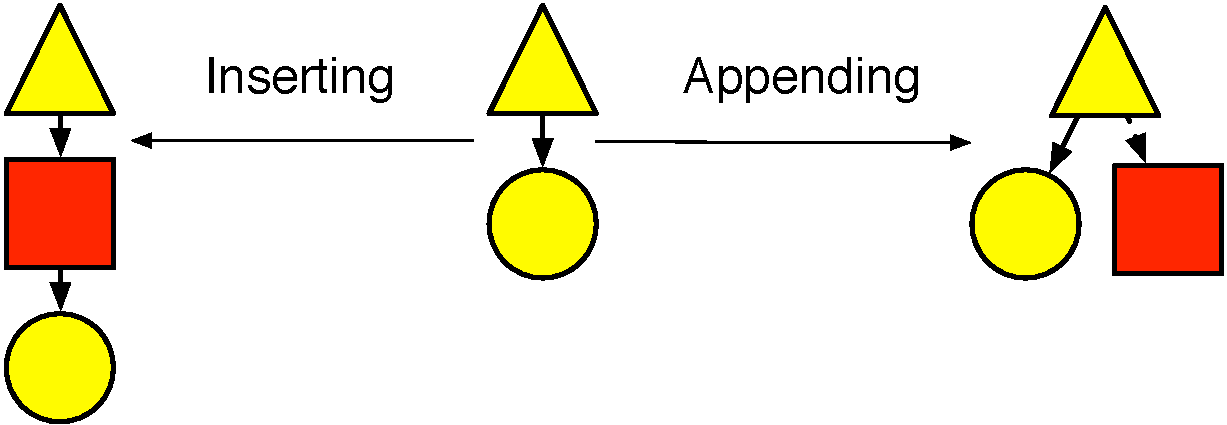
\epsfig{file=parameters/figures/both.pdf, width=4in}
\caption[Appending or inserting a generator to the hierarchy.]{Appending or inserting a generator to the hierarchy.
Module types are represented as shapes, and the newly inserted or appended modules are red.}
\label{fig:both}
\end{figure}

\begin{figure}
\centering
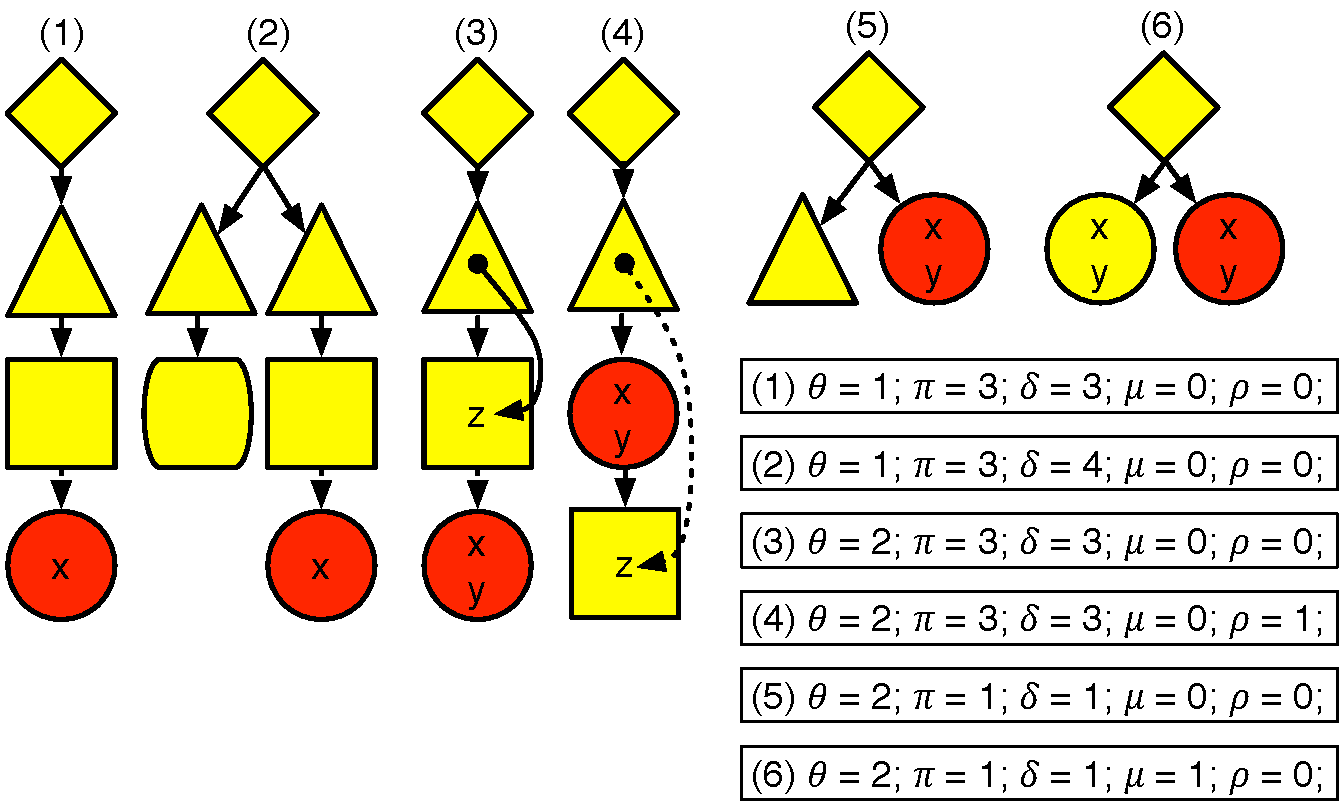
\epsfig{file=parameters/figures/CDSq2.pdf, width = 6in}
\caption[Example classifications of modifications.]{(1)-(6) are example module hierarchy modifications. 
Module types are shapes, the newly inserted or appended modules are red, and inter-module parameter references are curved arrows.}
\label{fig:attr}
\end{figure}

Section \ref{sec:tax} and Section \ref{sec:cde} used the case study of a tile generator to qualitatively contrast the efficacy of all five parameterization paradigms
at dealing with some specific modifications to the structure and hierarchy of hardware generators.
In this section, we instead attempt to analytically describe the robustness of each paradigm to \textit{any possible set} of design modifications.
The results show that using CDEs \textit{always} results in a more robust design according to our metric,
but they also provide insight into when other paradigms could be equally appropriate.

As in the previous sections, we define robustness as the number of source code changes that cascade from making a modification to an existing design
consisting of a hierarchy of generators that elaborate hardware modules.
We generalize the initial modifications into one of two categories: appends or insertions.
An \emph{append} is when a new generator is incorporated as a leaf node whose instantiations do not affect the overall organization of the existing module hierarchy
(e.g. the addition of \code{PFPU} in Section \ref{sec:tax}).
In contrast, an \emph{insertion} is when a new generator is incorporated between an existing parent and child node in the hierarchy (e.g. the addition of \code{CacheWithPF}). 
Insertions change the overall structure of the module hierarchy.
See Figure~\ref{fig:both} for an illustration of this distinction.

We assume all parameters added as part of a modification each require a unique value to be bound to their identifier at the top-level of the module hierarchy.
In other words, multiple copies of the same generator must be capable of being assigned different parameter values.
These unique bindings must then be brought into the scope of the place where the parameters are evaluated.
Therefore, each original modification will trigger a varying number of scoping-related source code changes,
depending on both the existing module hierarchy as well as the parameterization paradigm being employed.

In order to characterize how many source code changes of each type will be required for each class of modification under each parameterization paradigm,
we define the following attributes of a modification that introduces a new module, $M$, to the hierarchy:
\begin{itemize}%\itemsep1pt \parskip0pt \parsep0pt
\item $\theta$, the number of parameters used by $M$.
\item $\pi$, $M$'s depth in the module hierarchy.
\item $\delta$, the number of times any parent generator of $M$ is instantiated.
\item $\mu$, whether any other instances of $M$'s type exist.
\item $\rho$, the number of references to $M$'s children's parameters from any of $M$'s parents.
\end{itemize}

Figure \ref{fig:attr} depicts six examples calculating these attributes for different module hierarchies
In (1), a new module $M$ with one parameter is appended to a 3-level hierarchy with each level being of a unique type.
In (2), a module with one parameter is appended to a 3-level hierarchy where one of its ancestors is instantiated twice ($\delta = 4$), and the other two are instantiated once each.
In (3), a module with two parameters is appended to a 3-level hierarchy with a cross-module reference ($\theta = 2, \rho = 0$).
In (4), a module with two parameters is inserted into a 3-level hierarchy with a cross-module reference ($\rho = 1$).
In this case, $M$'s parent has a single reference to a parameter that is contained in $M$'s child.
In (5), a module with two parameters is appended to a 1-level hierarchy alongside a sibling of a different type than $M$ ($\mu = 0$).
In (6), a module with two parameters is appended to a 1-level hierarchy alongside a sibling that is the same type as $M$ and therefore uses the same parameter names internally ($\mu = 1$).

\begin{table}
\centering
\begin{tabular}{llll}
\toprule
Paradigm    & LC & NLC & Total Changes\\
\midrule
arg-lists      &  1              & $(\delta+\pi)*\theta$ & $1+\theta*(\delta+\pi+1)$  \\
flat-struct    &  1              & $\pi*\theta$          & $1+\theta*(\pi+1)$  \\
nested-struct  &  1              & $1+\rho$              & $2+\theta+\rho$  \\
regular-env    &  $1+\mu*\theta$ & 0                     & $1+\theta*(1+\mu)$ \\
CDE            &  $1+\mu$        & 0                     & $1+\theta+\mu$  \\
\bottomrule
\end{tabular}
\caption[Models of source code change.]{
Models of source code change for appending or inserting a module under any parameterization paradigm.}
\label{tab:limit}
\end{table}

Given these attributes, we can calculate the number of top-level, non-local, and local changes per modification type under each paradigm.
Table \ref{tab:limit} lays out analytical models for each combination.
Top-level changes are always equal to the number of parameters added by the modification ($\theta$).
Local changes consist of instantiating the new module and local manipulations of the module's parameter bindings.
Non-local changes include any other modifications, including parent instantiations, parent declarations, modifying any parent's parameter object's instantiation/declaration,
and correcting references to parameters in parent modules.
Total changes are simply the sum of all LCs, NLCs, and TLCs.

We begin by breaking down the NLCs required under each paradigm.
The arg-list paradigm requires $(\delta+\pi)*\theta$ NLCs, because each of $\theta$ parameters must be threaded through the declarations ($\pi$) and instantiations ($\delta$) of all of its parent modules in the hierarchy.
The flat-struct paradigm reduces this overhead to $\pi*\theta$ because the $\delta$ instantiations now refer to the struct instead of the individual parameters.
The nested-struct paradigm requires only $1+\rho$ changes; a single change to the declaration of the parent module's companion struct, as well as $\rho$ changes based on how many
references to parameters in $M$'s children there are in all of $M$'s parents.
If we are appending $M$ rather than inserting it, $\rho$ will of course equal 0 because there cannot be any references to nonexistent children.
The dynamically-scoped solutions require no NLCs, because the bindings created by the TLC are automatically put within the scope of $M$.

As for LCs, the lexically-scoped paradigms each only require a single LC, simply instantiating the module in question.
In the case of the dynamic environments, more than one LC is needed to both instantiate the module and differentiate the parameter bindings if necessary.
In particular, we use $\mu$ to indicate whether $M$ is instantiated anywhere else in the design hierarchy.
If it is, we must now differentiate the top-level bindings that are to be used for each instance of $M$
and re-map those bindings onto the identifiers used within $M$ as we instantiate it.
For regular environments, we introduce $\theta$ additonal LCs, because every new parameter needs to be renamed in order to disambiguate it from that of its peers.
For context-dependent environments, only a single additional LC is required, assuming the existence of a single geographical parameter whose value can be overridden for the new module.

The terms in these models help to clarify the kinds of tradeoffs we are making when we offer developers the opportunity or advice to use a particular parameterization paradigm.
For example, from the perspective of the author of a generator that will serve as the ``leaf'' node in the hierarchical graph of instantiations, there is no reason not to use argument lists.
However, as that generator becomes embedded within deeper and deeper generator hierarchies, the burden born by all the parent generators grows and grows, as captured by the $\pi$ term.
In fact, $\delta$ has an even larger potential to grow, since it is based on the number of different instantiations made anywhere in the source code,
rather than the number of parent generator constructor declarations represented by $\pi$.
The $\rho$ term governing nested-structs is highly design dependent, but it is an important signifier of the work that has been done within a design to ensure composability
by making assertions about the behavior and configuration of child generators.
In other words, more robust nested designs will have higher values of $\rho$.


The $\mu$ term captures whether the module being added is reusing parameter identifiers that are being used elsewhere.
It only matters for dynamically-scoped paradigms, because they must provide their own namespaces for identifiers, independent of the module hierarchy's lexcical scope.
In cases where we are heterogeneously adding an instance of a new module type or homogeneously adding an identical instantiation of an existing module type, no further work needs to be done.
Otherwise, each parameter must be uniquified as the module is instantiated.
Overall, we are making an argument that the $\delta$, $\pi$, and $\rho$ terms are the ones most likely to grow,
as well as the fact that NLCs are much more difficult to resolve than LCs because they could occur anywhere in the overall source codebase.

Despite the poor scalability of argument lists, all designs with a shallow module hierarchy are manageable with them, because the number of potential modifications is itself limited. 
Designs with shallow but wide hierarchies that have expect no insertions and have few cross-module parameter references (e.g. networks) could be made robust with the nested-struct paradigm,
assuming the number of child parameters is not itself determined by a parameter.
Deep hierarchical designs with minimal module reuse (e.g. processor pipelines) must support insertions as well as appends, but the diversity of the module types involved means there will be few parameter namespace collisions. These designs will remain robust with regular environment passing.
Complicated designs with deep hierarchies, significant module reuse, and many cross-module references that must address all flavors of appends and insertions (such as our SoC generator) clearly benefit from CDEs.

This analysis is predicated on the idea that the design in question will undergo further development and be deployed in new contexts,
but that agenda is central to our agile approach to hardware development.
The qualitative benefits of using CDEs extend beyond modifiability to composability and reusability.
While CDEs have disadvantages as well, we discuss how these can be mitigated through good software engineering practices in the following sections.

\section{Implementation of CDEs in Scala}
\label{sec:impl}

We will now provide some specifics about our implementation of Context-Dependent Environments in Scala.
After an overview of functionality offered by our CDE implementation, we will discuss the Scala language features we employed to create it,
as well as provide some insights into how we integrate CDEs with Chisel-based hardware generators.

At a high level, the values returned by identifiers stored in a CDE are not constant, rather they are functions whose arguments are:
\begin{description}
\item[pname,] the name of the parameter being queried.
\item[site,] the CDE against which the query was originally made.
\item[here,] the CDE currently being defined.
\item[up,] the last CDE created before this alteration.
\end{description}
The function bound to a particular identifier can choose to ignore the \code{site}, \code{here}, and \code{up} arguments and just return a constant value,
which provides the same functionality that would be found in a regular environment.
However, the use of more sophisticated parameter valuations based on querying \code{site} and the others
allows users to create chains of parameter dependencies and easily specialize deeply nested portions of their designs.
Scala provides some language features that significantly informed our implementation of this construct,
particularly first-class functions and partial functions, as well as typed dispatch via match statements.

\subsection{Environments as Partial Functions}

\begin{figure}
\centering
\begin{scala}
val fraction: PartialFunction[Int, Int] =
  { case d: Int if d != 0 => 42 / d }

val statusHandler: Int => String = {
  case 200 => "Okay"
  case 400 => "Your Error"
  case 500 => "Our error"
}

val config: PartialFunction[String, Any] = {
  case "size" => 32
  case "name" => "divider"
  case "func" => fraction
}

\end{scala} 
\caption{Partial functions in Scala.}
\label{fig:pf}
\end{figure}

At an abstract level, environments are associative arrays (also called key-value stores, maps, or dictionaries) wherein identifiers are bound to particular values.
Scala provides a \code{map} collection as part of its standard collections library, but we chose to use an even more fundamental built-in primitive as the basis of our CDE implementation:
partial functions.
In a mathematical context, a partial function provides a function  $f: X' \rightarrow Y$ for some subset $X'$ of $X$. If $X' = X$ we would call $f$ a total function.
The critical feature of a partial function is that we can define it without knowing the exact domain $X'$.

Scala provides first class support for functions (and partial functions), meaning that they are not only declared and invoked 
but can be used in every segment of the language as just another data type. 
A first-class function may be~\cite{swartz2014learning}:
\begin{itemize}
\item created in literal form without ever having been assigned an identifier;
\item stored in a container such as a value, variable, or data structure; or
\item used as a parameter to another function or used as the return value from another function.
\end{itemize}
Figure~\ref{fig:pf} shows some examples of partial functions defined as function literals.

The applicability to maps is obvious, and in fact, Scala provides built-in functionality for converting between map data structures and first class partial function types.
Our CDEs are built on top of this capability by composing hierarchies of partial functions that map from an identifier
to a parameter value (or Scala object created using multiple parameters).
Our framework is permissive about what type of Scala objects can be used as an identifier, accepting \code{Any} Scala type.
We can then use the pattern matching tools built in to Scala to match certain parameter names and extract additional information that may be stored in them.
Figure~\ref{fig:paramspf} provides some examples of making use of different types of identifiers and alterations.

\begin{figure}
\centering
\begin{scala}
val p1 = Parameters.empty.alter(Map("a" -> 1))
val a = p1[Int]("a")

val p2 = p1.alterPartial({"b" => 2})
val b = p2[Int]("b")

case class Location(x: Int, y: Int) extends Field[String]

val p3 = p2.alterPartial({
  case Location(x, 1) => "y is 1, x is " + x
  case Location(1, y) => "x is 1, y is " + y
})

val s = p3(Location(0,1))
\end{scala} 
\caption{Using partial functions and maps to bind parameter values.}
\label{fig:paramspf}
\end{figure}

We provide the \code{Field} wrapper class to improve the syntax for looking up a particular identifier, 
allowing us to elide declaring the expected return type on each lookup of the identifier.
By giving the identifier its own Scala class, we also can leverage the Scala type system to check that identifiers from different projects to do not conflict.

The values returned by our framework can also be of \code{Any} Scala type.
The framework uses the type specified in the \code{Field} definition 
or the one provided by the user at the query site
to dynamically cast the value obtained from the environment to the intended type.
This cast can fail at runtime if the wrong type of object is provided, an inherent weakness of our dynamic scoping approach.

Partial functions can naturally be composed with one another. If an identifier fails to match
within a certain context, we can catch the \code{MatchError} thrown and then go on to search
in the remaining ones.
We exploit this functionality to create hierarchies of environments,
where modifying a parent creates a child with new bindings that can override the parent's bindings,
and which in the absence of new bindings will fall back on the parent's bindings.

\subsection{site, here, and up}

\begin{figure}
\centering
\begin{scala}
val p1 = Parameters.empty

val p2 = p1.alter(
  (key, site, here, up) => key match { 
    case "width" => 64
    case "double" => here("width") * 2  // here reference
    case "hetero" => site("loc") match {
      case Location(x, 1) => "In core location #" + x
      case Location(y, 2) => "In uncore location #" + y
    }
  }
) 

val core1 = Module(new Core(p2.alter("loc" -> Location(1,1))))
val core2 = Module(new Core(p2.alter("loc" -> Location(2,1))))
val uncore = Module(new Uncore(p2.alter("loc" -> Location(1,2))))

\end{scala} 
\caption{Using \code{site}, \code{here} and  \code{up} for context-dependent parameterization.}
\label{fig:site}
\end{figure}

As discussed in the previous section, the fundamental additional feature of a CDE over a regular environment is a special object,
called \emph{site}, that dynamically points to the originating CDE of the parameter query.
\emph{site} is available to be queried when defining the value bound to a particular identifier.
In other words, environment values bound within the environment are no longer mere constant literals, instead
they have been promoted to functions which take as an argument a dictionary representing the view of the world as seen from the query's point of origin.
When the environment is asked to evaluate a particular parameter identifier, the function stored for that key in the dictionary is evaluated against the dictionary itself.
We call parameters that use the \emph{site} functionality {\em context-dependent} because the valuations taken by their bindings depend on where the query is made.
We call \emph{site} itself a \emph{view} of the environment.

In addition to the view from \code{site}, we also provide users attempting to alter their environments with the views called \code{here} and \code{up}.
\code{site} gives the user access to parameter valuations based on the value they have been defined to have to the call site.
\code{here} gives the user access to parameter valuations that are being defined within the very same alteration statement.
\code{up} gives the user access to parameter valuations that were available in the previous, unaltered version of the environment.
Figure~\ref{fig:site} shows examples of how \code{site}, \code{here}, and \code{up} can be used to evaluate parameters based on their particular view of the environment.

\subsection{Constraints}

\begin{figure}
\centering
\begin{scala}
case object NClients extends Field[Int]

class MyScalableNetwork extends Module {
  params.constrain( ex => ex(NClients) >  0 ) 
  ...
} 

class MyTinyNetwork extends Module {
  params.constrain( ex => ex(NClients) > 0 && ex(NClients) <= 4 )
  ...
} 

class MyPairsNetwork extends Module {
  params.constrain( ex => ex(NClients) > 0 ) 
  params.constrain( ex => ex(NClients) <= 32 )
  params.constrain( ex(NClients)\%2 === 0 )
  ...
} 
\end{scala} 
\caption{Constraining parameter values. }
\label{fig:constraints}
\end{figure}

As the author of a hardware generator library, it is important to expose to external users (e.g., SoC architects)
not only the free parameters of the design, but also any constraints that must be placed on
the values bound to those parameters. 
While preventing illegal parameter bindings from producing incorrect designs can be done with elaboration-time assertions
in the generator source code, we feel a better strategy is to give SoC authors enough information
so as to avoid even attempting to generate bad designs in the first place.

We provide a constraint expressions library that operates on \code{Fields}.
Users can deploy this library to create simple expressions that describe relationships between parameters.
Figure~\ref{fig:constraints} shows some examples of constraint expressions.
Within any \code{Module} or \code{Bundle} component of our library, we can constrain the values of arbitrary fields using these expressions
and register them using the \code{constrain} function.
We support a set of expressions compatible with many constraint solving tools %($===, +, -, *, \%, <, >, <=, >=, \&\&, ||, ^$), 
as well a range checking bound.

In addition to using constraints as runtime assertions while elaborating a particular hardware design instance,
we also experimented with extracting them from a design during elaboration and serializing them
to an external format compatible with a constraint solving tool.
When using the Chisel compiler in this mode, at least one safe set of parameter bindings must be known
(we discuss a mechanism for encoding safe default values in the next subsection).
As we elaborate a design instance using these default parameters, we record all the constraints
registered by the compiler.
This set of constraints can then be fed to an external tool capable of enumerating all legal parameter bindings.
This enumerated design space can then be explored in order to find the optimal design point for a particular workload or metric.

\subsection{External Interfaces}

\begin{figure}
\centering
\begin{scala}
class DefaultConfig extends ChiselConfig { 
  val topDefinitions:World.TopDefs = { 
    (pname,site,here) => pname match { 
      case NTiles => Knob('NTILES') 
      ...
    } 
  } 
  override val topConstraints:List[ViewSym=>Ex[Boolean]] = List(
    ex => ex(NTiles) >= 1 && ex(NTiles) <= 8 && (ex(NTiles)\%2 === 0 || ex(NTiles) === 1)
  )
  override val knobValues:Any=>Any = { 
    case 'NTILES' => 1 // generator parameter assignment 
  } 
} 

class With2TilesConfig extends DefaultConfig {
  override val knobValues:Any=>Any = { 
    case 'NTILES' => 2
  } 
} 

\end{scala} 
\caption{ChiselConfigs and Knobs.}
\label{fig:configs}
\end{figure}

We provide two further abstractions as part of our Scala CDE library, both focused on interactions with external tools.

\code{Knobs} are hooks intended for use by design space explorers using CDEs to inject parameters into a design.
They provide another level of name binding indirection available within the top-level definitions (\code{TopDefs})
of a \code{Parameter} environment.
They essentially serve as meta-parameters to which multiple other parameters' names can be bound, depending on the
use case of the exploration process.
Knobs values are automatically flagged to be dumped to external files when a particular design instance is created using them.

\code{ChiselConfigs} are representations of complete or partial parameter bindings, associated with a particular name and expressed using Scala source code.
\code{ChiselConfigs} consist of the three primary components potentially needed to elaborate a design instance based on CDEs:
top-level \code{Parameter} definitions, \code{Knob} value bindings, and top-level \code{Constraints}.
We chose to express configurations via Scala source code rather than an external serialization format for economy of design.
Given the name of a \code{ChiselConfig} sub-class, we can instantiate it using Scala's reflection capabilities and feed the \code{Parameters} thereby generated to Chisel.
\code{ChiselConfigs} can extend one another through Scala's multiple inheritance as well as be composed by name dynamically.
Figure \ref{fig:configs} provides a simple example of \code{ChiselConfig} definition and inheritance.




\section{Parameterization Best Practices In Chisel}

The goal of this section is to distill some of the learned wisdom about effective software engineering strategies
for deploying CDEs in a Chisel-based hardware generator.
Beyond which parameterization paradigm to use,
there are additionally a wide variety of design decisions that aid the process of injecting parameters into a design.
In particular, Scala provides several built-in features that we exploit, which are not innately coupled to our choice of using
CDEs for paramterization but do complement it.
The following subsections attempt to capture some of the tradeoffs we have explored while taping out chips using our SoC generator.

\subsection{Scala's Implicit Parameter Lists}

\begin{figure}
\centering
\begin{scala}
class A(implicit p: Parameters ) extends Module {
  val w = p[Int]("width")
}

class B(implicit p: Parameters) extends Module {
  val a16 = Module(new A) // A's constructor's implicit parameter resolves to p
  val a32 = Module(new A(p.alterPartial({"width" => 32})))
}

val b = Module(new B(Parameters.empty.alter(Map("width" -> 16}))))
\end{scala} 
\caption[Using Scala's implicit parameters.]{Using Scala's implicit parameters to pass Parameter instances to Modules when no fields are overridden.}
\label{fig:implicit}
\end{figure}

Implicit parameters are a form of lexical scoping that offer some of the perks of dynamic scoping in a limited (but safe) context.
They are another built-in feature of the Scala language.
When a method or constructor declares one of its parameters as \code{implicit}, 
users of that method can decide whether or not to supply a value for that parameter.
In cases where no explicit value is supplied, the compiler automatically searches the context
of the method call for a matching ``implicit'' value.
Resolution rules for implicit parameters guarantee that only a single matching value will be allowed to be bound by the compiler.
The salient feature of the \code{implicit} resolution rules is that they are based on only
a single value of a matching type being marked with the \code{implicit} keyword in lexical scope.

Implicit parameters simplify Scala APIs by eliding parameters with which standard users do not need to concern themselves.
In our case, we have found them to be particularly useful for passing our \code{Parameters} objects through a hierarchy of Modules and Bundles.
In cases where none of the Parameter fields are being altered (which is the common case),
users do not have to explicitly pass the \code{Parameter} instance into the Module or Bundle's constructor.
Figure~\ref{fig:implicit} shows examples of how implicit parameters are expressed in Scala and how we use them to make \code{Parameters}
available throughout a hardware Module hierarchy.
  
\subsection{Scala Traits and Mix-ins}

\begin{figure}
\centering
\begin{scala}
trait HasTileLinkParameters {
  val p: Parameters // Abstract member
  val co = p[CoherencePolicy]("TLCoherencePolicy") // Parameters bound to local vals
  val nM = p[Int]("TLNManagers")
  val nC = p[Int]("TLNClients")
  val dataBits = p[Int]("TLDataBits")
  val dataBeats = p[Int]("TLDataBeats")
  val dataBitsPerBeat = dataBits / dataBeats // Derived parameter
}

trait HasCacheParameters {
  val p: Parameters // Abstract member
  val nSets = p[Int]("NSets")
  val nWays = p[Int]("NWays")
}

class MyBundle(implicit val p: Parameters) extends Bundle // Concrete type
    with HasTileLinkParameters {                          // supplies p for trait
  val data = UInt(INPUT, width = dataBits) // Use a val from the trait
}

class MyCache(implicit val p: Paramaeters) extends Module
    with HasCacheParameters
    with HasTileLinkParameters { // Multiple inheritance
  val io = new MyBundle // Implicit parameter passed here
  val managers = for (i <- 0 until nM) yield { ... }
  val sets = for (i <- 0 until nSets) yield { ... }
}
\end{scala} 
\caption{Using traits to factor out and mix in parameter bindings.}
\label{fig:mixin}
\end{figure}

Scala supports multiple inheritance, wherein member definitions of multiple classes can be reused in the definition of a new class.
This multiplicity is accomplished without inheritance ambiguity by way of {\em mixins},
which are classes that contain methods for use by other classes without having to be the parent class of those other classes.
Specfically, Scala allows users to define mixin {\em traits}
that represent a distinct feature or aspect orthogonal to the responsibility of a concrete type.
A trait cannot itself be instantiated, instead the trait's functionality is mixed-in when defining or using a class.
Since traits are innately abstract, they can contain abstract methods and members that are to be filled in by the concrete class.

We have found it productive to use traits to encapsulate the process of extracting parameter values from CDEs and binding them to local variable names.
Parameter lookups need only occur once per class instantiation instead of every time a particular parameter is used.
Code reuse is improved across many classes that make use of the same parameters, such as all the Bundles in
a multi-channel protocol specification.
Figure~\ref{fig:mixin} shows examples of how we mix-in traits containing parameter bindings to Module and Bundle sub-classes.

\subsection{Case Classes versus Fields}

\begin{figure}
\centering
\begin{scala}
// Using Fields

class TLCoherencePolicy extends Field[CoherencePolicy]
class TLNManagers extends Field[Int]
class TLNClients extends Field[Int]
class TLDataBits extends Field[Int]
class TLDataBeats extends Field[Int]

trait HasTileLinkParametersFromFields {
  val p: Parameters
  val co = p(TLCoherencePolicy)
  val nM = p(TLNManagers)
  val nC = p(TLNClients)
  val dataBits = p(TLDataBits)
  val dataBeats = p(TLDataBeats)
  val writeMaskBits: Int = ((dataBits / dataBeats) - 1) / 8 + 1
  val dataBitsPerBeat: Int = dataBits / dataBeats // Derived parameter
}

// Using case classes

case class TileLinkParameters(
    coherencePolicy: CoherencePolicy,
    nManagers: Int,
    nClients: Int,
    dataBits: Int,
    dataBeats: Int = 4,
    overrideDataBitsPerBeat: Option[Int] = None
    ) {
  val writeMaskBits: Int  = ((dataBits / dataBeats) - 1) / 8 + 1
  val dataBitsPerBeat: Int = overrideDataBitsPerBeat.getOrElse(dataBits / dataBeats)
}

class TLKey extends Field[TileLinkParameters]

trait HasTileLinkParametersFromStructs {
  val p: Parameters
  val tl = p(TLKey)
  val co = tl.coherencePolicy
  val nM = tl.nManagers
  val nC = tl.nClients
  val dataBits = tl.dataBits
  val dataBeats = tl.DataBeats
  val writeMaskBits = tl.writeMaskBits
  val dataBitsPerBeat = tl.dataBitsPerBeat
}
  
\end{scala} 
\caption[Two alternative approaches to representing sub-fields.]{
Two alternative approaches to representing sub-fields of interrelated parameters.
In the first example, we use \code{Fields} representing individual parameters, and relate them inside of a \code{trait}.
In the second example, we use a \code{case class} that wholly encapsulates the parameters and their relationships.
}
\label{fig:fields}
\end{figure}

Another parameterization design decision that is orthogonal to the choice of paradigm is
the granularity with which individual parameters are exposed to the rest of the design.
Figure~\ref{fig:fields} shows two alternative approaches that generator authors can take to expose
the parameters used by their generator to external clients.
Each approach has pros and cons, and designers using our tools have employed each in different instances.

In the first approach, every independent parameter is represented by an individual \code{Field} definition.
Dependent parameters are then defined in traits after the parameters have been bound to local variables.
This approach plays nicely with our \code{Constraints} framework,
which relies on individual parameters being referenced in the expressions built up to describe a constraint.
However, it requires users to mix-in the traits to gain access to their members that are storing parameter values.
It also imposes an additional burden when we work with context-dependent parameters, as we will discuss
in the next subsection.

In the second approach, every independent parameter is made a member of a case class.
Scala case classes export their constructor parameters,
provide a succinct syntax for copy constructors,
and provide a recursive decomposition mechanism via pattern matching.
Dependent parameters are defined within the class itself.
This approach is not as compatible with our \code{Constraints} framework, which at this time
does not support constraints defined on individual class members.
However, it provides all dependent parameters inherently, requiring no mixins.
It also provides a convenient syntax for working with context-dependent parameters.

\subsection{Geography and Heterogeneity}

\begin{figure}
\centering
\begin{scala}
case object CacheName extends Field[String] // New geographical fields
case object TLId extends Field[String]

class DefaultConfig extends Config(
  topDefinitions = { (pname,site,here) =>
    pname match {
      case "NSets" => 128 // A context-independent (constant) lookup
      case "NWays" => if(site(CacheName) == "L1I") 2 else 4 // A context-dependent lookup
      case TLKey => if(site(TLId) == "L2ToMC") {            // and another
          TileLinkParameters(
            coherencePolicy = new MEICoherence(new NullRepresentation(site(NBanksPerMemoryChannel))),
            nManagers = 1,
            nClients = site(NBanksPerMemoryChannel),
            dataBits = site(CacheBlockBytes)*8)
        } else {
          TileLinkParameters(
            coherencePolicy = new MEICoherence(new NullRepresentation(site(NBanksPerMemoryChannel))),
            nManagers = 1,
            nClients = site(NBanksPerMemoryChannel),
            dataBits = site(MemoryInterfaceBytes)*8)
        }
      //...
    }
  }
)

// Inject geography into context
val l2toMCNetwork = Module(new TLNetwork()(params.alter({TLId => "L2toMC"})))

// A different location
val outerNetwork = Module(new TLNetwork()(params.alter({TLId => "Outermost"})))

// Can be multiply located
val icache = Module(new ICache()(params.alter({CacheName => "L1I"; TLId => "L2toMC"})))

\end{scala} 
\caption{Using CDEs to express geographical heterogeneity.}
\label{fig:geo}
\end{figure}

Figure~\ref{fig:geo} shows examples of how geographical information can be embedded in a CDE
and exploited by making use of the \code{site} functionality.
For each parameter that varies heterogeneously across the design, we use \code{site}
to reference another parameter that abstractly describes the ``location'' of that parameter within the design.
Parameters that vary together are keyed off of the same geographic parameter.
It is important to note that the original generator library does not need to know anything about
this geographical parameter:
it can be introduced by external users and injected into the design at the top-level or anywhere in between.
\code{site} is what allows us to decouple the definition of the parameters' bindings from the run-time evaluation of their values,
which vary based on ``where'' they are queried.

\subsection{The FindBy Pattern}

\begin{figure}
\centering
\begin{scala}
case object CacheName extends Field[String]
case object TLId extends Field[String]
case class TLKey(id: String) extends Field[TileLinkParameters]

class DefaultConfig extends Config(
  topDefinitions = { (pname,site,here) =>
    type PF = PartialFunction[Any,Any]
    def findBy(sname:Any):Any = here[PF](site[Any](sname))(pname)
    pname match {
      case "NSets" => findBy(CacheName) // Pivot to lookup by cache name
      case "NWays" => findBy(CacheName) // Likewise
      case "L1I" => { // Icache location
        case "NSets" => 128
        case "NWays" => 2
      }:PF
      case "L1D" => { // Dcache location
        case "NSets" => 128
        case "NWays" => 4
      }:PF
      case TLKey("L2toMC") => // First
        TileLinkParameters(
          coherencePolicy = new MEICoherence(new NullRepresentation(site(NBanksPerMemoryChannel))),
          nManagers = 1,
          nClients = site(NBanksPerMemoryChannel),
          dataBits = site(CacheBlockBytes)*8)
      case TLKey("Outermost") => site(TLKey("L2toMC")).copy(dataBeats = site(MemoryDataBeats))
      //...
    }
  }
)
\end{scala} 
\caption{Using a transformation to collate related parameters in a Config based on geography.}
\label{fig:findby}
\end{figure}

While allowing each parameter to vary independently based on geographical parameters is a powerful capability,
in practice many sets of parameters vary together because they are controlling the same generator.
We have found that users are often discontent with varying each of these correlated parameters independently.
When many locations are possible for each parameter, the replicated code to select among them can
take up a significant fraction of the Config description. 
Figure~\ref{fig:findby} shows examples of other strategies for managing correlated parameters.

The first method we introduce we term the \code{findBy} pattern. We add a utility function that
makes use of both \code{site} and \code{here} in order to pivot the parameter lookup such that we first lookup
the geographic key and then within that namespace lookup the original parameter query.
This pivot has the effect of allowing us to organize parameter bindings that change in the same way
so as to be sorted by geographical location.

The second method performs a similar transformation, but builds on the earlier design decision
to use case classes to store related parameters rather than individual fields.
This pattern is concise and allows us to make use of the copy constructor syntax built into case classes, because we
can reference other geographic keys directly.
In cases where we do not need to define constraints on individual parameters, we find we prefer this syntax.
However, this is more of a stylistic choice than a functional one, as the two approaches
are functionally equivalent.

We will return to some of these examples in later chapters after we define further properties of TileLink networks and CoherencePolicies.

\section{Discussion and Future Work}
\label{sec:con}

Unlike high-level synthesis tools that transform abstract descriptions of a computation into gates,
hardware generators are parameterized, programmatic descriptions of how to elaborate a templated RTL module hierarchy.
Because parameters are so essential to generators, we have devoted significant effort to
developing a parameterization paradigm that supports composing them.
As we look forward, we envision Chisel serving as the basis on which more abstract and high-level tools will be layered.
We contend that parameterization will be just as important for such tools.
Even though some of the details of the implementation may become hidden,
we will need to provide direction for how the high-level computations should be mapped
onto hardware structures.
Furthermore, the space of possible implementations for a HLS description can be quite large,
so expressing those tradeoffs in a way that is compatible with design space exploration is important.

While I will not discuss it further as part of this thesis, we have prototyped some initial implementations
of hooking up our \code{Parameters} and \code{Constraint} abstractions to a design space exploration tool called Jackhammer.
Given a set of free top-level parameters and a set of constraints placed upon them, Jackhammer can create a design of experiments and
execute that design against a cloud-based service for design point evaluation.
Further work is required to automate the exploration process and close the loop between feedback from one iteration of examining a
set of design instances and selecting points for further exploration.

The biggest downside to relying on a dynamically-scoped solution for parameterization is that there
is a class of errors that would be compile-time errors in a lexically-scoped system that are
run-time errors in a dynamically-scoped one.
These errors include things such as:
parameters never being bound to a value, function, or \code{Knob};
parameters being bound to return a type that does not match that expected by their query site;
or infinite recursion of the CDE implementation due to loops in the \code{site} call graph.
While we have attempted to provide sensible error messages for some of these cases,
it is difficult to wholly absolve ourselves of introducing the possibility of run-time failures.
In the future, it might be possible to use Scala's support for macros to do a better job of eliding the need for runtime type casts
in cases where the top-level configuration is itself specified as Scala source code.
Overall, we feel that the power of dynamic scoping for modification of parameters in deeply nested hierarchies,
such as those seen in our RocketChip generator, is worth the cost.

\section{Conclusion}
\label{sec:con}

We have presented a taxonomy of existing parameterization paradigms in HDLs and demonstrated that our 
context-dependent environments paradigm is provably more robust in the face of modification to any given design's module hierarchy. 
We have also provided case studies of how CDEs are particularly appropriate for hardware generators
and offered insights into how best to deploy them within a new HDL embedded in Scala.
In the following chapters, we will move on to the specifics of how to express cache coherence protocols with hardware generators
and build on the CDE framework to effectively parameterize both the protocols themselves and the hardware modules that implement them.

\chapter{TileLink: A Protocol Substrate for Coherence Policy Transactions }
\label{c.tilelink}

TileLink is a protocol framework designed as a substrate for multiple cache coherence policies.
Its purpose is to separate the design of the communication network and the implementation of the cache controllers from the design of the coherence protocol itself.
This separation of concerns improves the modularity of the HDL description of the memory hierarchy,
while also making validation and verification of individual memory system components more tractable.

Any cache coherence protocol that conforms to TileLink's transaction structure can be used interchangeably alongside the physical networks and cache controllers we provide.
By supplying a framework to apply transactional coherence metadata updates throughout the memory hierarchy, TileLink enables simplified expressions of the coherence policies themselves.
Conversely, as long as newly designed controllers and networks make certain guarantees about their behavior,
system-on-chip designers can be confident that incorporating them into their TileLink-based memory hierarchy will not introduce coherence-protocol-related deadlocks.
As part of the Rocket Chip Generator project, I have supplied an initial library of cache controllers and on-chip physical networks that conform to this TileLink specification.

TileLink is roughly analogous to the data link layer in the IP network protocol stack, but exposes some details of the physical link necessary for efficient cache controller implementation.
This tradeoff avoids imposing any deserialization overhead on data being refilled between levels of an on-chip cache hierarchy, while also allowing for data bus widths
that are tractable to place-and-route between the different caches in the hierarchy.
Despite the emphasis on on-chip deployment, TileLink is suitable for implementing a coherence protocol in a multi-chip system as well.

TileLink is designed to be extensible and supports a growing family of custom cache coherence policies.
TileLink also codifies a set of transaction types that are common to all protocols.
In particular, it provides a set of transactions to service memory accesses made by agents that do not themselves have caches containing coherence policy metadata.
These built-in transactions make TileLink a suitable target for the memory interfaces of accelerators, co-processors and DMA engines,
and allow such agents to automatically participate in a global shared memory space.

TileLink is hierarchical, in that protocols based on it can be nested inside one another.
This structure comports well with the tree-based structure of on-chip cache hierarchies.
Memory requests that cannot be satisfied within a particular hierarchy level are translated into the protocol assigned to the next-outermost level. 
TileLink uses a variation on the Manager-Client Pairing framework~\cite{beu2011manager}
to provide encapsulation and translation between levels.

The rest of this chapter lays out the case for TileLink and provides a detailed specification of its architecture.
I discuss the assumptions and guarantees made by the various components of a TileLink system and explain how components implementing them interact
to supply deadlock and starvation-free, coherent, global shared-memory implementations.
Details of how specific coherence policies extend TileLink are discussed in Chapter~\ref{c.coherence}.

\section{Background}

In a system with hardware-managed cache coherence, the cache controllers and memory controllers
communicate among themselves according to some protocol to maintain coherence.
While they might have vastly different implementations, 
all such protocols maintain coherence by ensuring the same {\em single-writer, multiple-reader} (SWMR) invariant \cite{sorin2011primer}. 
For a given block of cached memory, at any given moment in logical time, there is either: 
(1) a single core that may write and read the block, or 
(2) there are zero or more cores that may only read the block.
However, because this definition is based on a notion of logical time rather than physical time,
it does not preclude a variety of important optimizations that would otherwise appear to violate this constraint.
Our definition of coherence must also augment the SWMR invariant with a data value invariant
that pertains to how values are propagated from one logical epoch to the next.
This invariant states that the value of a memory location at the start of an epoch
is the same as the value of the memory location at the end of its last read-write epoch \cite{sorin2011primer}.
Violating either of these invariants could lead to values written by one core never becoming visible to other cores.

For the rest of this chapter, I distinguish coherence policies from coherence protocols.
A coherence {\em policy} governs how the SWMR invariant is represented as metadata identifying available permissions on data blocks and how to change those permissions.
A coherence {\em protocol} specifies the exact flows of messages and state updates that must be propagated through the memory hierarchy in order to effect a policy.
In other words, a policy specifies what access permissions are possible and when those permissions should be changed,
whereas a protocol specifies how any changes are communicated to the rest of the hierarchy.
TileLink provides a single coherence protocol {\em template} on top of which many policies can be implemented.
A particular cache coherence policy will specify permissions changes that must occur as a result of a serialization of memory operations.
Using these policy-based decisions to fill in the TileLink template results in a complete coherence protocol.

A protocol comprises a specified set of allowable interactions between any agents that access copies of blocks of shared memory.
A ``transaction'' made up of a subset of these interactions effects a single memory operation at the policy level,
and a complete protocol will include many such transactions.
We term legal sets of interactions between agents ``transactions'' because the SWMR invariant must be preserved,
even though the permissions metadata being accessed is distributed throughout the hierarchy.
Futhermore, all agents must agree on the serialization of permissions changes to a particular block.
The distributed agents must achieve consensus about permission states and data values
despite the fact that there may be no ordering guarantees
provided by the underlying communication network, and so no trivial notion of global serialization of the transactions.
Increasing memory operation throughput by allowing multiple transactions to be in-flight through the cache hierarchy
at the same time is essential to efficiency, but significantly increases the complexity of the protocol implementation.

The transactions that make up a coherence protocol tend to assume a particular shape depending on what
assumptions are built into the underlying message transport network they rely upon.
Figure~\ref{fig:hops} shows how certain transport assumptions result in different numbers of messages sent per transaction and different points of serialization.
In Figure~\ref{fig:hops}.A, by exploiting a globally synchronous broadcast medium (such as a bus), client agents can directly reply to one another in only two hops.
When only point-to-point communication is available (Figure~\ref{fig:hops}.B), a manager agent provides a possible point of synchronization, as well as forwarding certain filtered messages to other clients.
However, those clients then respond to the transaction originator directly.
If the point-to-point network cannot guarantee ordered message delivery, transactions can include a fourth hop (Figure~\ref{fig:hops}.C)
that will add latency, but which provides opportunities for more fine-grained concurrency control to maintain a global serialization.
The symmetry of a four-hop transaction style also enables hierarchical composability in multi-level memory systems.
TileLink is based around a four-hop structure.

\begin{figure}[t!]
\centering
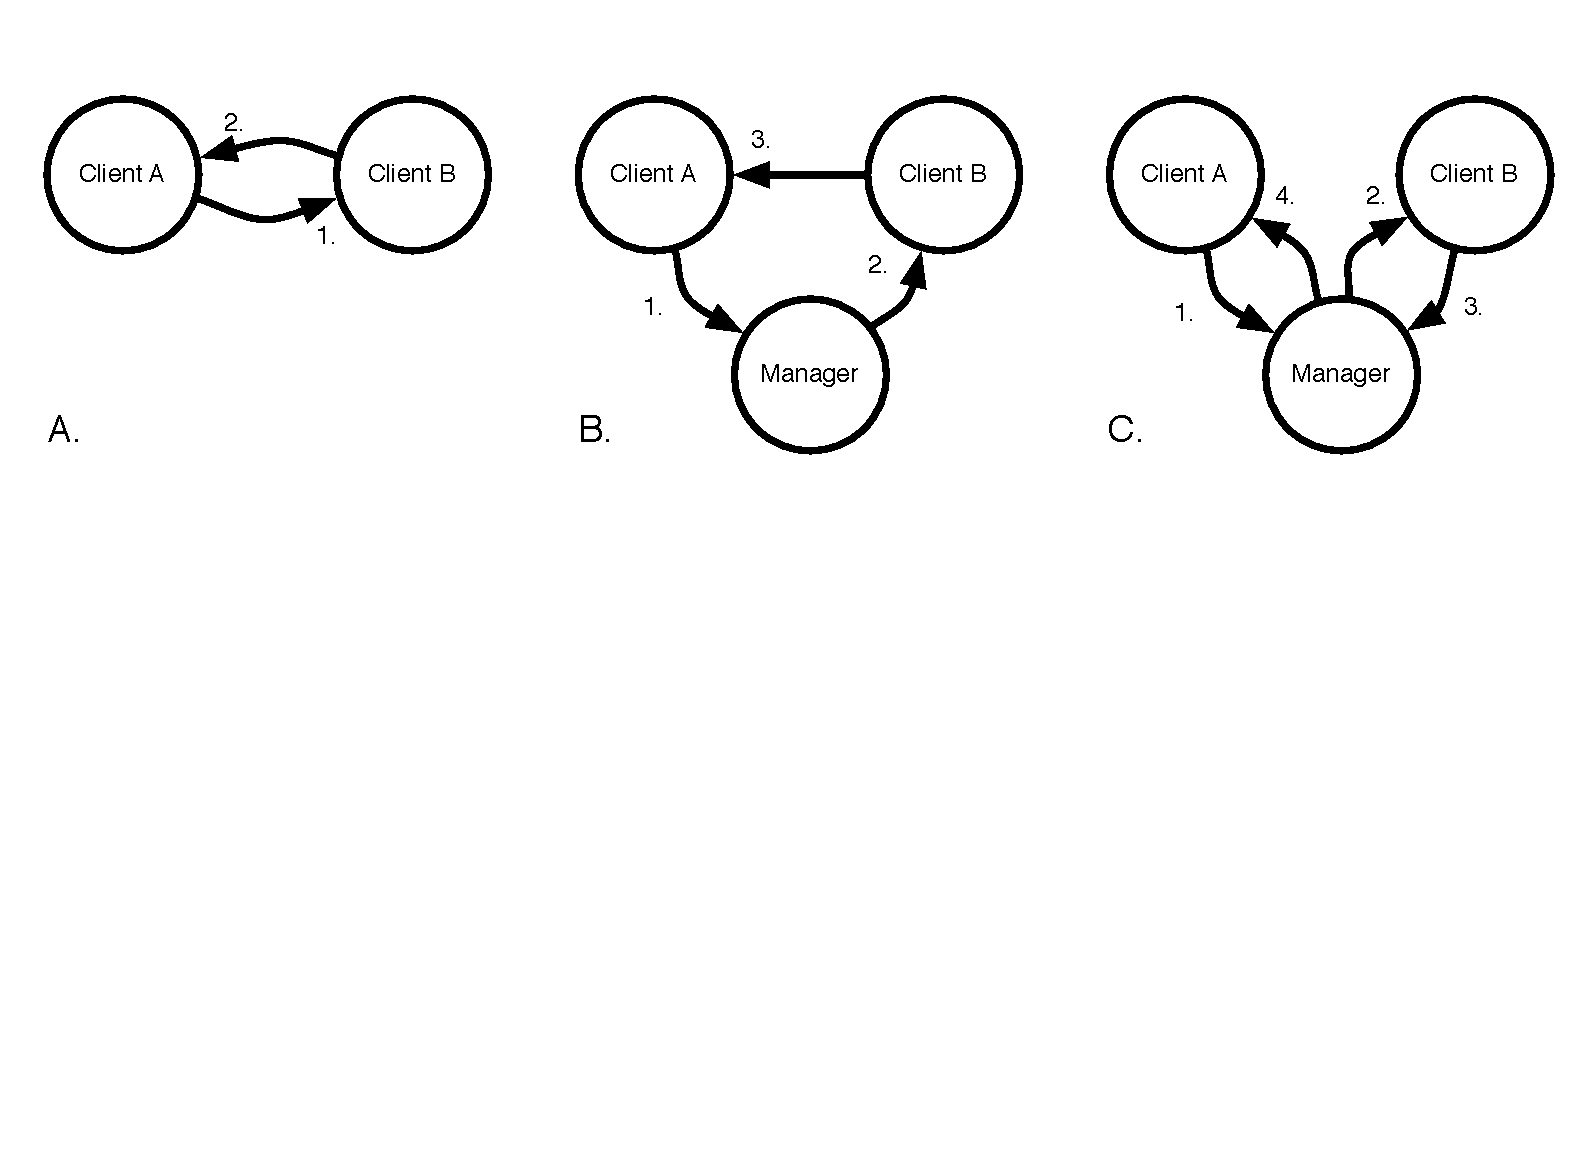
\includegraphics[width=1\columnwidth]{tilelink/figures/hops.pdf}
\caption[Sketches of various coherence transaction shapes.]{
Sketches of various coherence transaction shapes.
A. Exploiting a globally synchronous broadcast medium, client agents can directly reply to one another in two hops.
B. With point-to-point communication, a manager agent provides a possible point of serialization.
C. With unordered message delivery, a fourth hop can symplify the complexity of maintining a global serialization.
}
\label{fig:hops}
\end{figure}

Thus far we have discussed the concepts that inform the behavior of TileLink within a single level of the memory hierarchy.
In order to extend TileLink to support protocols that span multiple levels of the hierarchy, we apply a variation of the Manager-Client Pairing (MCP) framework \cite{beu2011manager}.
MCP defines an interface between users of data (client agents) and the mechanisms that monitor coherence of these users (manager agents) on the two sides of a coherence protocol interface.
A given agent can act also as both a client and a manager, and serve as the bridge between two nested realms of the multi-level coherence protocol.
Figure~\ref{fig:mcp} shows how this strategy can be applied in a divide-and-conquer manner to arbitrarily deep hierarchies
by carving them up into nested coherence realms.
Applying the MCP framework to a memory sytem is advantageous because it provides
encapsulation within each tier of the hierarchical protocol,
which in turn mitigates the state-space explosion
that makes multi-level protocol designs prohibitively expensive to verify.
Standardization and encapsulation enable more rapid
design of hierarchical coherence protocols via community-validated
building blocks that can be readily compared, tested and evaluated \cite{beu2011manager}.

\begin{figure}[]
\centering
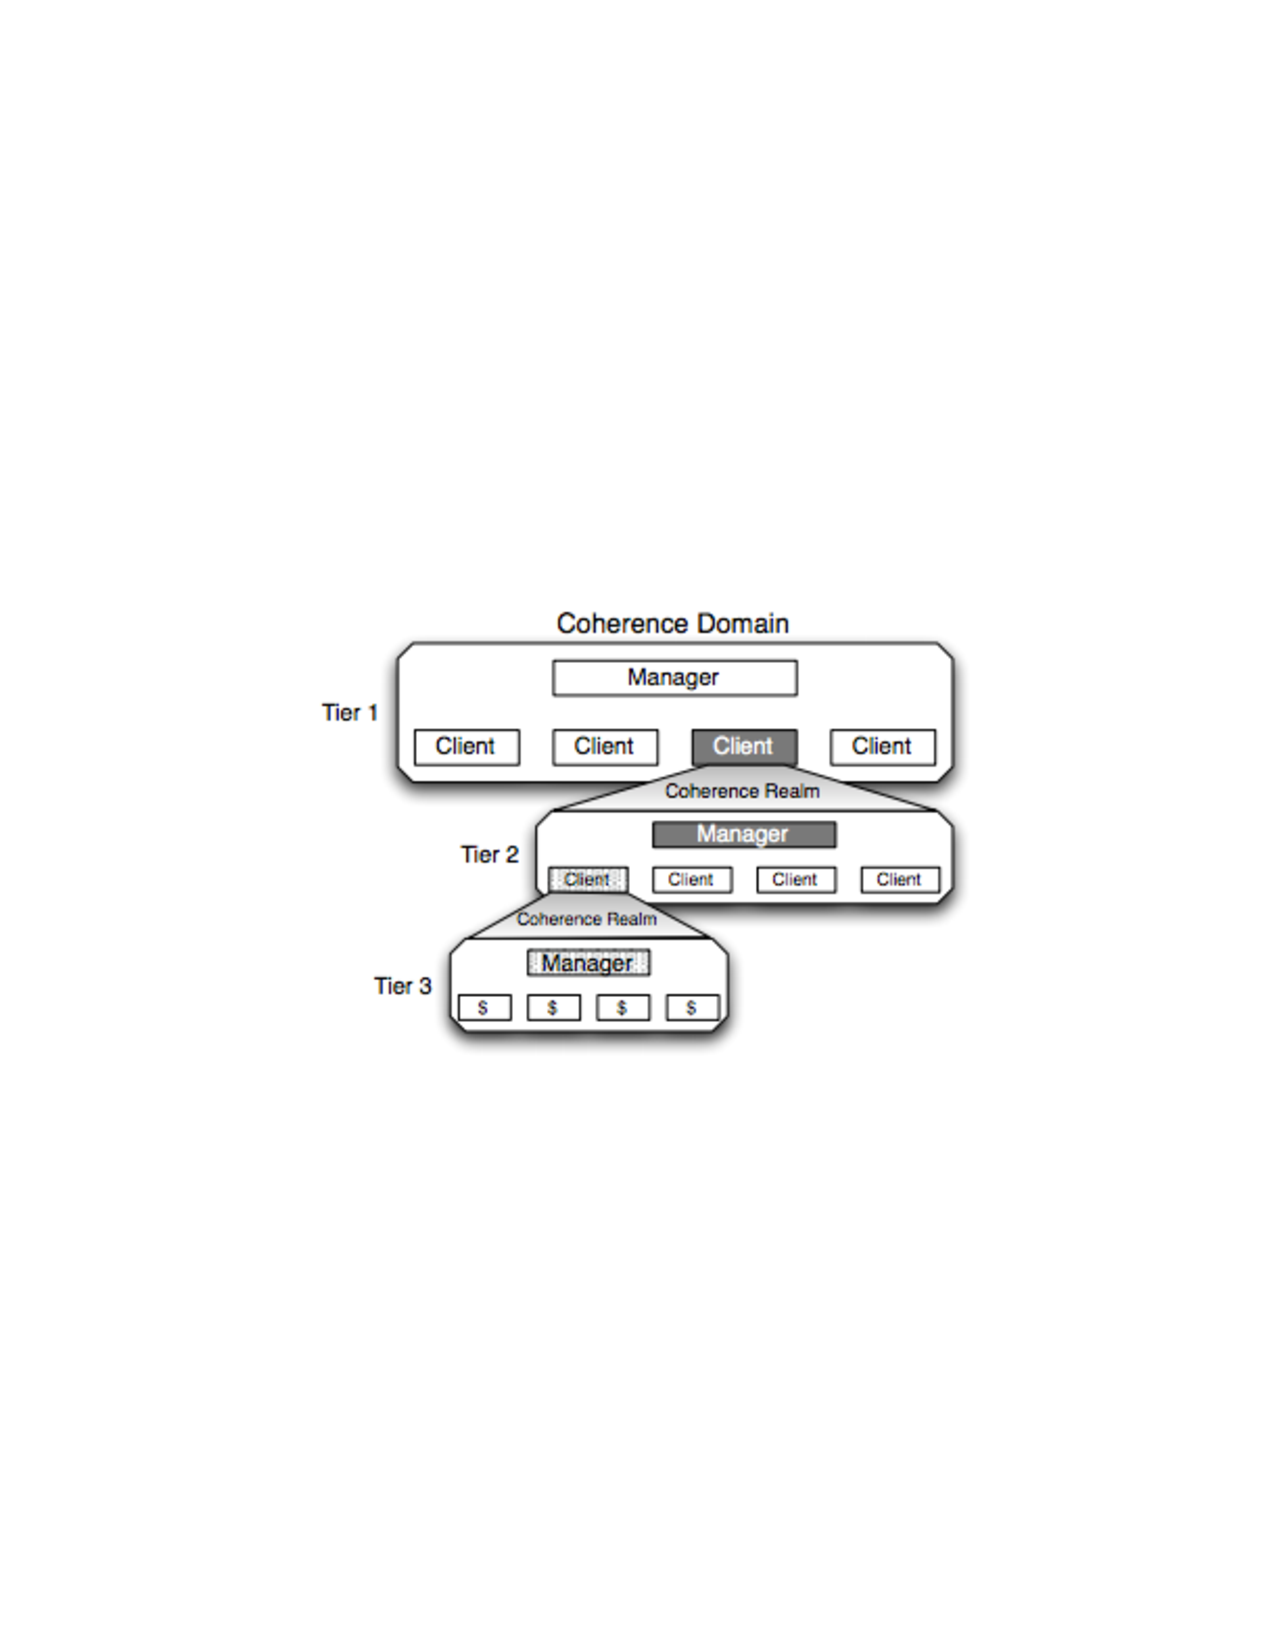
\includegraphics[width=1\columnwidth]{tilelink/figures/mcp-realm.pdf}
\caption[Nested coherence realms in the MCP paradigm.]{
Nested coherence realms in the MCP paradigm. 
The innermost realm consists of client agents and their manager, which may in
turn be the client of a second tier manager in an outer realm, and so on.
Hierarchical agents act as both inward managers and outward clients. }
\label{fig:mcp}
\end{figure}

\section{Architecture}
\label{s.arch}

The fundamental components of the Tilelink specification are agents, channels, and transactions.
{\em Agents} are the active participants in the protocol that send and receive messages in order to access copies of data through the memory hierarchy.
Five independent {\em channels} transfer messages containing metadata and data between agents.
A {\em transaction} is a specific sequence of messages sent between agents via these channels
that cause certain agents to gain or lose permissions to access copies of cached data blocks.

TileLink is a hierarchical protocol, wherein a Manager-Client Pairing (MCP) methodology encapsulates the complexity of supporting
multiple levels of protocol within a single memory hierarchy~\cite{beu2011manager}.
Within any one level of the memory hierarchy, TileLink is based off of a symmetric, four-hop transaction structure (Figure~\ref{fig:hops}.C).
Manager agents serve as a point of serialization for coherence transactions on a block occuring within their coherence realm.
All messages sent to clients are eventually acknowledged, which allows the manager to ensure that all clients have
individually serialized transactions on a particular cache block in the same order.

TileLink tries to impose as few constraints as possible on the implementation of both the agents' controllers and the underlying physical network.
This design emphasis somewhat increases protocol complexity, but it makes TileLink applicable to a wide variety of physical design constraints and application domains.
With regards to agents, TileLink does not make assumptions about what state the agents are capable of storing about each cache block,
though it does require agents without state to operate in particular, conservative ways.
TileLink does not assume that messages are delivered in order between two particular endpoints by the underlying physical network,
though it does require an extra transaction message absent point-to-point ordering.
The ramifications of these design decisions are discussed in more detail in the following sections.

\subsection{Agents}

Agents are the active participants in the protocol that send and receive messages in order to transfer copies of data through the memory hierarchy.
Agents participating in the TileLink protocol are either:
\begin{description}
\item[Clients] that request permissions to read or write data within cache blocks, or
\item[Managers] that oversee the propagation of cache block permissions and data.
\end{description}

A client may be a cache, a DMA engine, an accelerator, or any other component that would like to perform memory operations in a coherent global shared memory.
Even clients that do not actually cache a copy of the data within themselves may use TileLink in order to see a coherent view of memory with respect to other clients that do have caches
(i.e., to see dirtied data currently stored in those clients, see Section~\ref{s.uncached}).
Clients are responsible for initiating transactions to gain or cede permissions on copies of cache blocks, and also for reporting on whether they possess certain permissions on those blocks
at the behest of their manager.

A manager may be an outer-level cache controller, a directory, or a broadcast medium such as a bus controller.
Managers may or may not posses a local copy of a data block themselves, but they must know how to source and supply data in response to their clients' requests.
In addition to supplying data, managers are responsible for tracking which clients have been granted which permissions on a data block,
and for probing those clients in order to ensure that the 
single-writer, multiple-reader (SWMR) invariant \cite{sorin2011primer} is upheld.
If a manager does not track the propagation status of individual blocks in precise detail it must be pessimistic
in terms of the quantity and type of probe messages that it sends.
A manager also provides a point of serialization for coherence transactions
initiated by any of the clients within its domain.

In a multi-level memory hierarchy with multiple nested realms of TileLink protocols, a particular agent can function as both
a client (with respect to caches further out in the hierarchy)
and a manager (with respect to caches closer in to the processors).
We term such an agent {\em hierarchical}.
These hierarchical agents must perform a translation of the various message types between the inner and outer protocol.
This translation process is described in more detail in Chapter~\ref{c.coherence}.
Hierarchical agents may or may not store a copy of the data locally, but they must at least track a set of ongoing transactions and serve as a serialization point for the inner protocol.

\subsection{Channels}

TileLink defines five independent transaction channels over which messages can be sent by agents in order to transfer information through the memory hierarchy.
These channels may be multiplexed over the same physical link, but to avoid deadlock, TileLink specifies a priority amongst the channels that must be strictly enforced.
Channels may contain both coherence metadata and actual copies of data.
The amount of data associated with and tracked by a piece of metadata within a particular level of TileLink is called a data {\em block}.

The channels are:
\begin{description}
\item[Acquire.] Initiates a transaction to acquire access to a cache block with proper permissions. Also used to write data without caching it locally.
\item[Probe.] Queries a client to determine whether it has a cache block or revoke its permissions on that cache block.
\item[Release.] Acknowledges probe receipt, releasing permissions on the block along with any dirty data. Also used to voluntarily write back dirty data.
\item[Grant.] Provides data or permissions to the original requestor, granting access to the cache block. Also used to acknowledge voluntary Releases.
\item[Finish.] Final acknowledgment of transaction completion from requestor, used for transaction serialization.
\end{description}

At the present time, all channels are routed from clients to their manager or from the manager to its clients.
Future extensions to TileLink may add support for client-to-client messaging.

The prioritization of channels is Finish >> Grant >> Release >> Probe >> Acquire, in order of decreasing priority.
Preventing messages of a lower priority from blocking messages of a higher priority from being sent or received is necessary to avoid deadlock~\cite{sorin2011primer}.
Since Finish messages must always be consumed by manager agents, overall forward progress in the system is guaranteed.

Every channel presents a decoupled interface, meaning that each contains ready and valid signals.
Ready is driven high by the recipient when it can accept a message over that channel,
and valid is driven high by the sender when it has a message to offer.

Channels that contain data may send the data over multiple {\em beats}, where each beat contains a subset of the block's data.
The relationship between the size of the data beat and the size of the data block is configurable.
Typically the lower bound of data block size is set based on
the desired ratio of metadata to data storage overhead,
while the upper bound is set by the diminishing returns on exploiting spatial locality in most programs,
as well as other cache coherence performance concerns that will be discussed in the next chapter.
The data beat size, in contrast, is set based on the width of the underlying physical network.
In the current implementation, thhe width of the underlying network is exposed to TileLink agents in order to
improve the efficiency of refilling data into caches whose data array rows are of a matching size to the network width.
Any agent generating messages that contain multiple beats of data is always responsible for incrementing the {\tt addr\_beat field}, as we will discuss in Section~\ref{s.types}.
Exposed beats are just one possible physical implementation of TileLink, and are independent from the overall transaction message flow organization.

\subsection{Transactions}

All changes in the coherence state can be understood as a series of transactions.
Each transaction consists of a series of messages sent between clients and their manager
and the actions that those agents take upon receipt of a particular message.
Typical agent actions are updating local metadata, forwarding the message to other clients, or supplying copies of data in response.
The overall outcome of a transaction is to change the permissions that some client has on a particular block.

We term these interactions ``transactions'' because the SWMR invariant must be preserved even though the permissions metadata is distributed throughout the hierarchy.
Futhermore, all clients must agree on the serialization of permission changes to a particular block.
The distributed agents must achieve consensus about permissions and data despite the fact that there are no ordering guarantees
provided by the channels, and so no trivial notion of global serialization of the transactions.

The directed acyclic graph (DAG) of messages sent and actions taken as part of a transaction is termed a ``message flow''~\cite{talupur2008going}.
The figures in this and the following sections plot message flows as message sequence charts,
which display the ordering and dependencies of the messages sent between agents and the actions they take in response over time.
In addition to providing an intuitive understanding of protocol behavior, message flows are also a potentially
rich source of behavior invariants that can be used for verification of protocol correctness, as will be discussed in Chapter~\ref{c.coherence}.

\begin{figure}[t!]
\centering
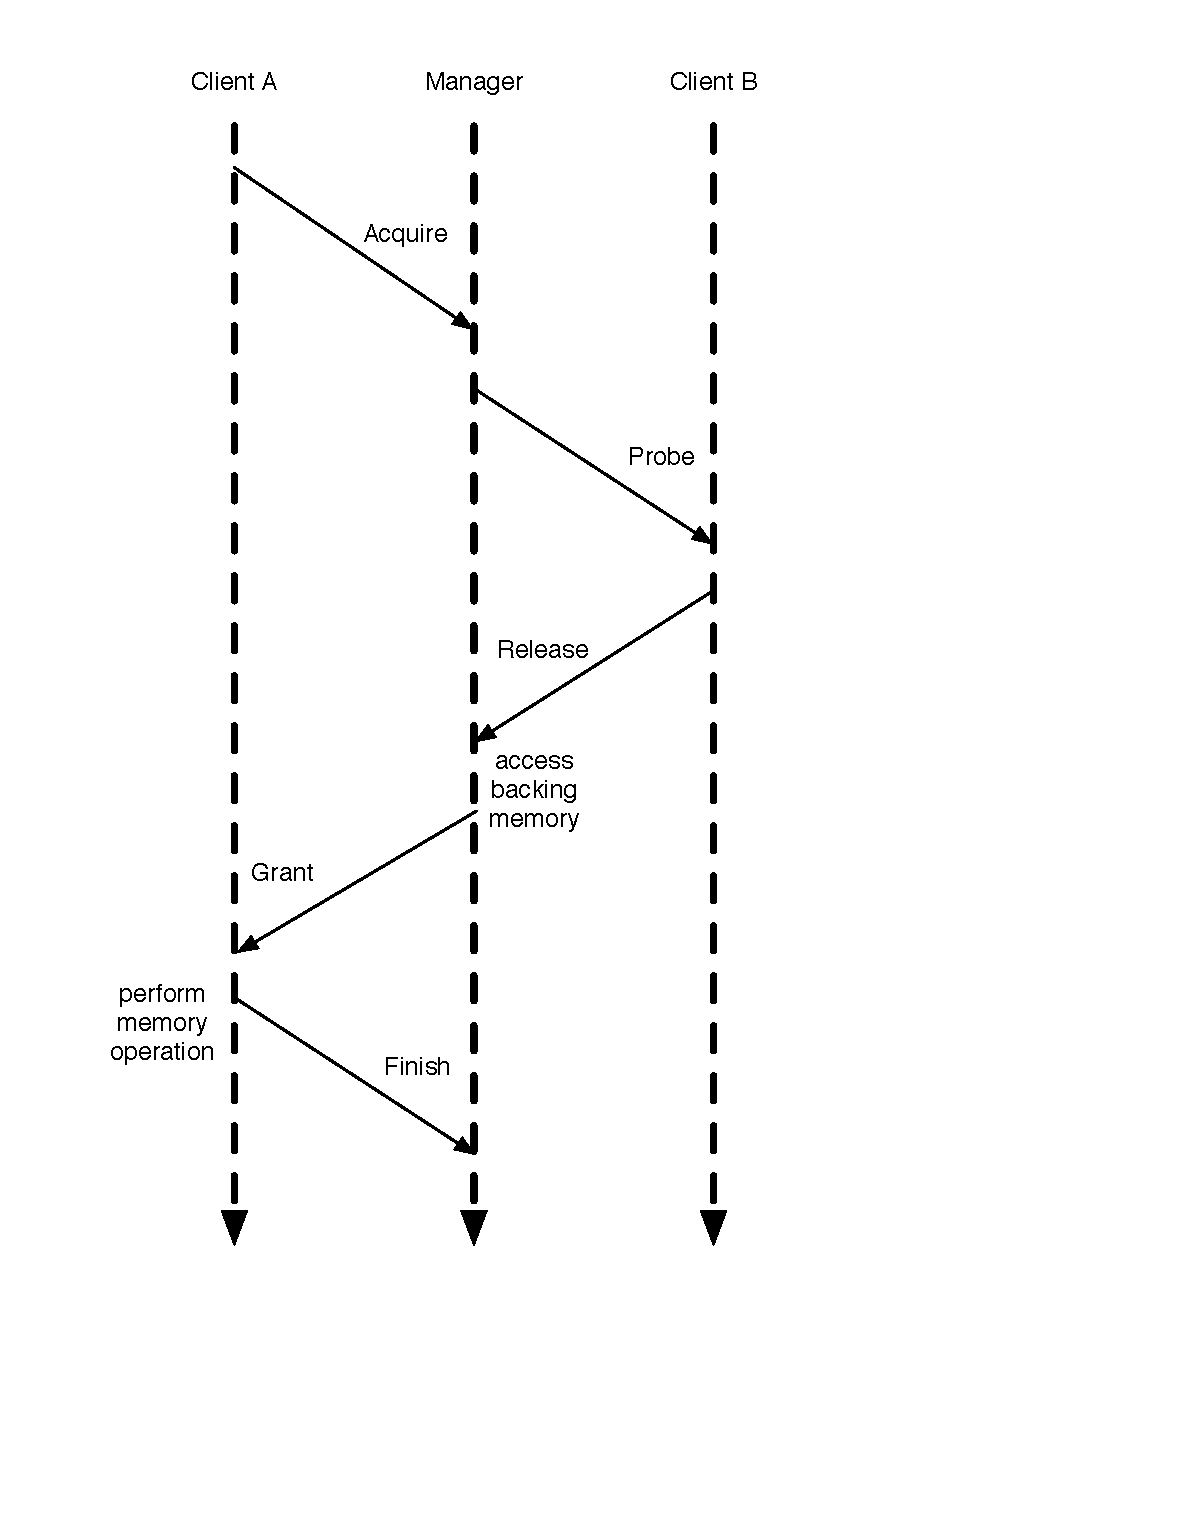
\includegraphics[width=0.6\columnwidth]{tilelink/figures/standard3.pdf}
\caption[Transaction flow to Acquire permissions on a cache block.]{
Overview of the transaction flow whereby a client acquires permissions on a cache block.
A client sends an Acquire to a manager.
The manager sends any necessary Probes to other clients.
The manager waits to receive a Release for every Probe that was sent.
The manager communicates with backing memory if required.
Having obtained the required data or permissions, the manager responds to the original requestor with a Grant.
Upon receiving a Grant, the original client responds to the manager with a Finish to complete the transaction.
}
\label{fig:standard3}
\end{figure}

There are two fundamental templates of transactions that can occur on a cache block managed by TileLink.
The first flow enables clients to acquire permissions to read or write data in a cache block.
Figure~\ref{fig:standard3} shows the message flow for this transaction in more detail.
After this transaction has completed, the client has acquired permissions to either read or write the cache block, as well as a copy of the block's data.
Other clients may have had to release their permissions on the block and write back dirty data in their possession.
If the manager is capable of tracking which clients have copies of the block using a directory, this metadata has been updated.

\begin{figure}[t!]
\centering
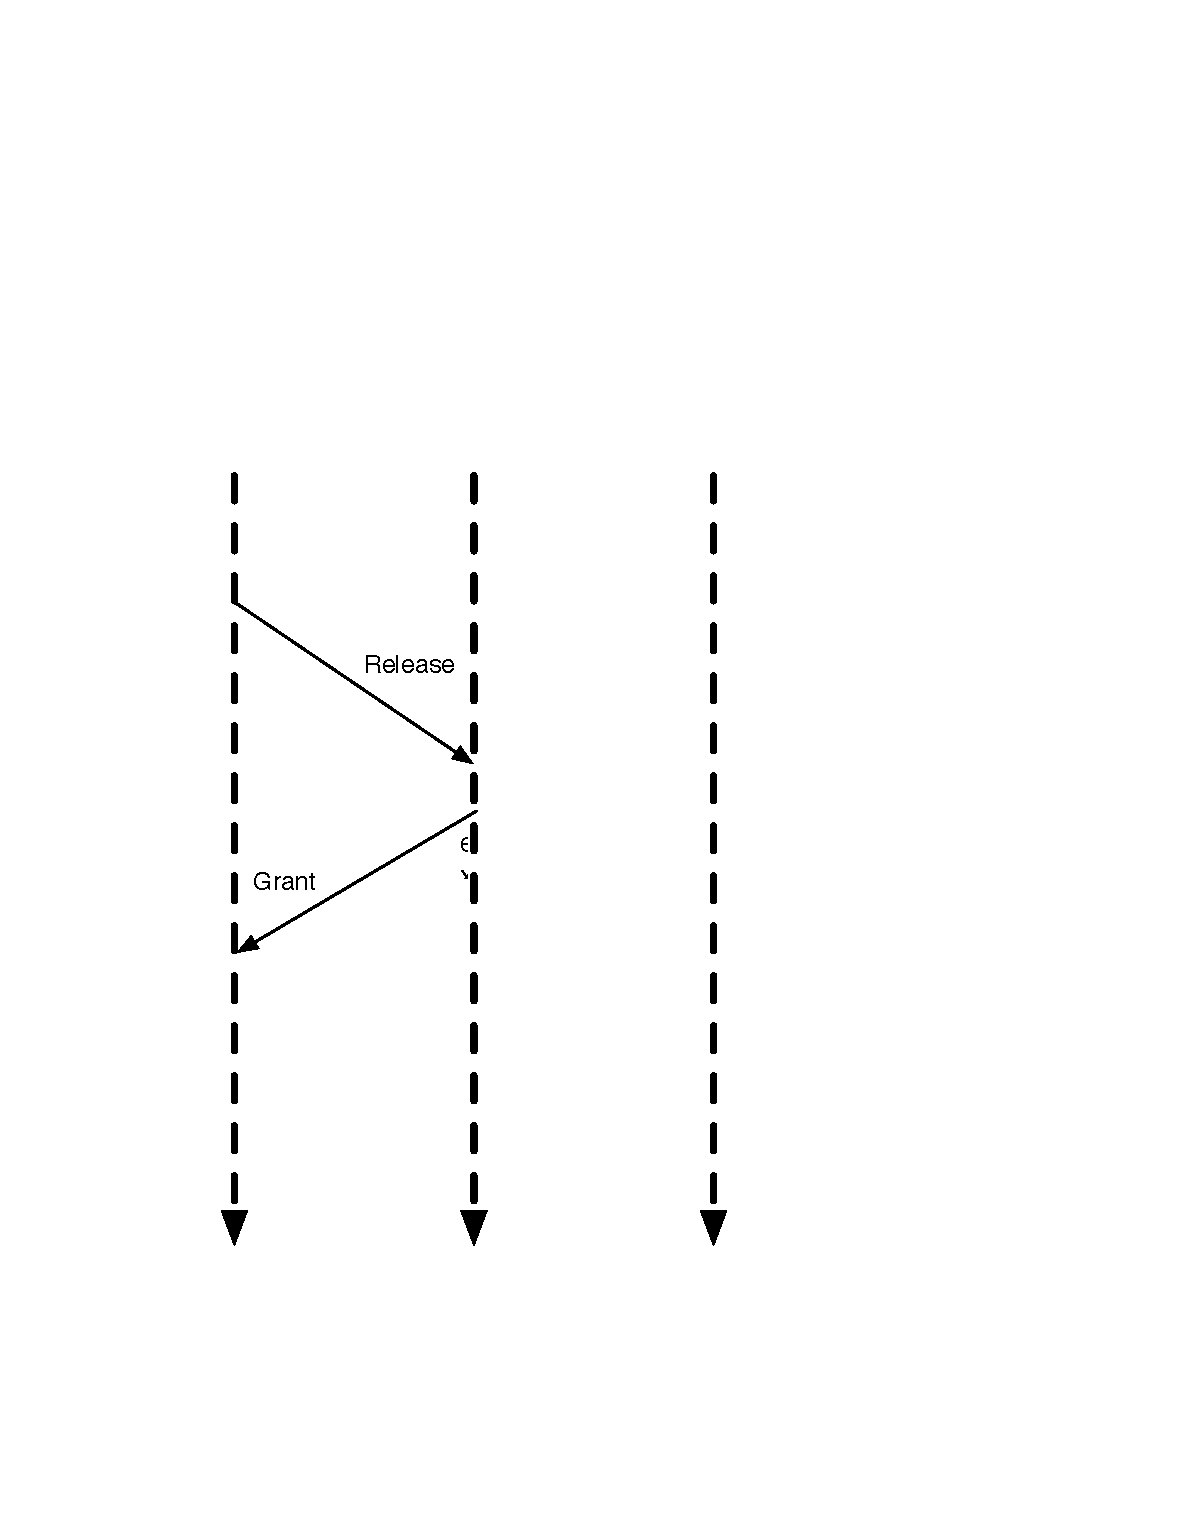
\includegraphics[width=0.5\columnwidth]{tilelink/figures/volwb.pdf}
\caption[Transaction flow to Release permissions on a cache block.]{
Overview of the transaction flow whereby a client voluntarily releases permissions on a cache block,
typically due to evicting the block for capacity reasons.
A client sends a Release to a manager, specifying that it is voluntary.
The manager communicates with backing memory if required.
The manager acknowledges completion of the transaction using a Grant.
}
\label{fig:volwb}
\end{figure}

The second type of transaction allows clients to voluntarily release their permissions on a cache block.
Figure~\ref{fig:volwb} shows the message flow for this transaction in more detail.
Typically, this type of transaction occurs when a cache must evict a block that contains dirty data, in order to replace it
with another block being refilled into the cache.
It might also be triggered by software hints, as we will discuss in Chapter~\ref{c.coherence}.
After this transaction has completed, the client has lost permissions to read or write the cache block, as well as its copy of the data.
If the manager is capable of tracking which clients have copies of the block using a directory, this metadata has been updated.

While these two flows form the basis of all TileLink transactions, there are a number of edge cases that arise when
they are overlaid on each other temporally or composed hierarchically.
The following sections discuss how responsibility for managing this complexity is distributed across the different TileLink agents.

\subsection{Concurrency in TileLink}

TileLink does not make any assumptions about the ordering of messages sent point-to-point over particular channels.
Therefore, concurrency must be managed by agents at several points in the system.
Imposing restrictions on agent behavior makes it possible for us to guarantee that a total ordering of transactions can be constructed,
despite the distributed nature of the problem and the lack of a global point of communication synchronization.
At the same time, we want to allow as much concurrency as possible among transactions whenever it is safe to do so.
There are three fundamental responsibilities to limit concurrency placed on TileLink agents:
\begin{itemize}
\item A manager should not accept another request for a transaction on a block that is already in-flight (unless it knows how to merge the two transactions as discussed below). Specifically, the manager must wait until it has received a Finish from the original client in order to ensure proper ordering of any future Grants on the same block to the same client.
\item If client has an outstanding voluntary writeback transaction, it cannot respond to an incoming Probe request on that block with Releases until it receives a Grant from the manager acknowledging completion of the writeback. It also cannot issue an Acquire on that block until it receives such a Grant.
\item If a client has an outstanding Acquire transaction, it should not issue further Acquires on that block unless they are of different types (for ``cached'' transactions)
or target different sub-block addresses (for ``uncached'' transactions). See Section~\ref{s.uncached} for details.
\end{itemize}

\begin{figure}[p]
\centering
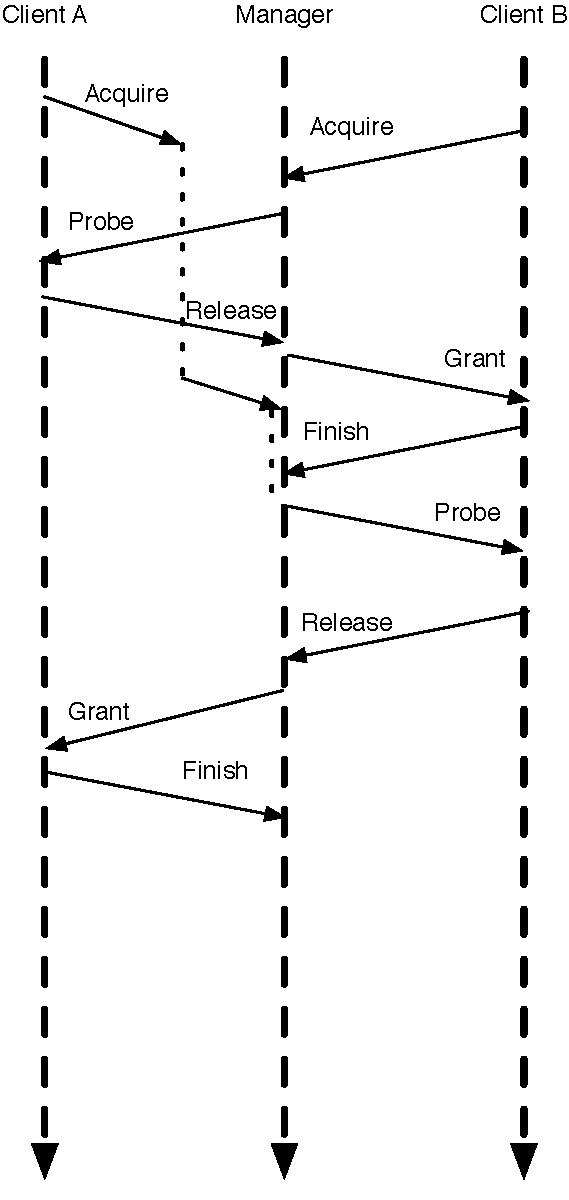
\includegraphics[width=0.5\columnwidth]{tilelink/figures/ordered.pdf}
\caption[Interleaved but well-ordered message flows.]{
Interleaved message flows demonstrating a manager blocking Acquires from multiple sources.
Clients A and B send an Acquire to a Manager, with Client B winning the race.
The manager blocks Client A's transaction from making forward progress.
Client A must process any Probes issues by Client B's transaction, even though Client A has an Acquire outstanding.
The manager must respond with the correct type of Grant (including a copy of the data), given that Client A has been Probed since sending its Acquire.
Once Client B responds with a Finish, Client A's transaction can proceed as normal.
}
\label{fig:ordered}
\end{figure}

\begin{figure}[!p]
\centering
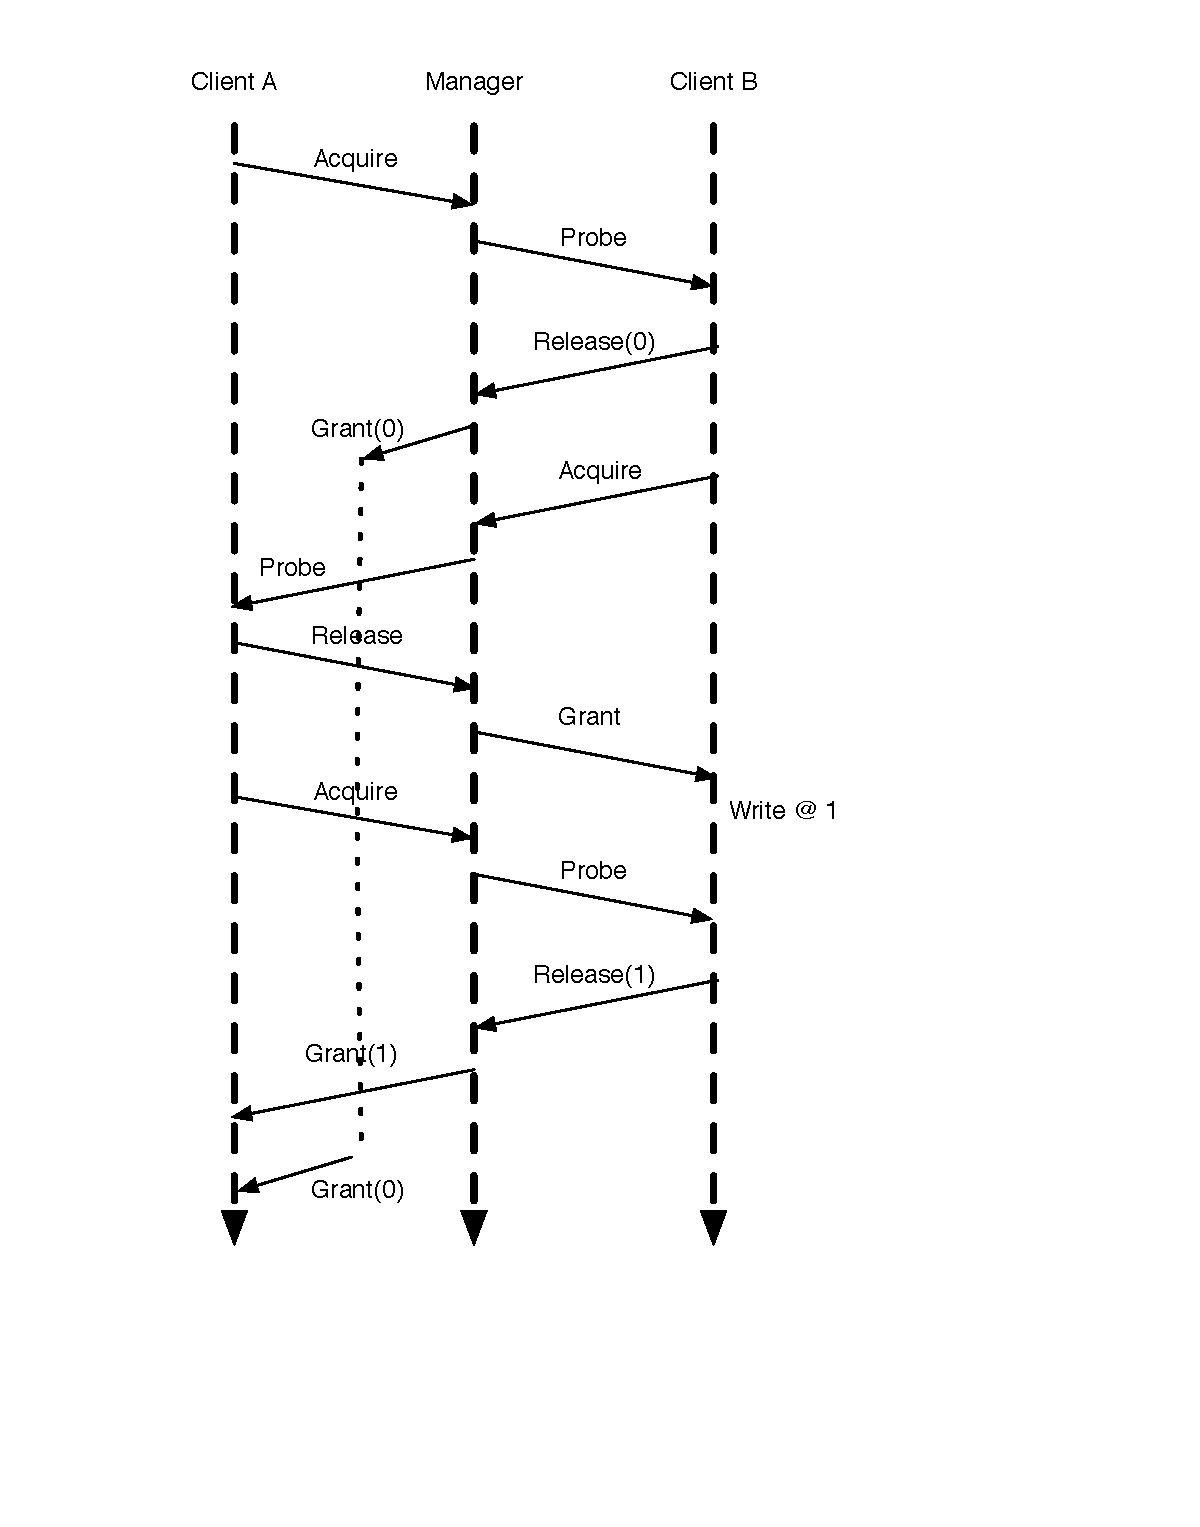
\includegraphics[width=0.5\columnwidth]{tilelink/figures/unordered.pdf}
\caption[Interleaved and disordered message flows.]{
Interleaved message flows demonstrating the need for Finishes to serialize Grant ordering.
Client A sends an Acquire to a manager, which in turn Probes Client B to Release dirty data.
This dirty data is forwarded by the manager in the form of a Grant to the transaction source, Client A.
Unfortunately, this Grant becomes delayed arbitrarily long in the unordered channel. 
Meanwhile, Client B initiates a transaction on the same block, Acquiring it in order to perform a write.
Client A must respond to the resultant Probe, even though it is still waiting for the missing Grant.
Client B is Granted permission to perform the write.
Client A then initiates a second transaction on the block, perhaps to upgrade its permissions, even though it is still waiting for the missing Grant.
Client B Releases the modified data, and it is Granted to Client A.
The second Grant bypasses the first Grant, and when the second Grant arrives, it overwrites the modified data with the original data.
Thus, from the perspective of Client A, the write to the block performed by Client B is lost.
}
\label{fig:unordered}
\end{figure}

\begin{figure}[!p]
\centering
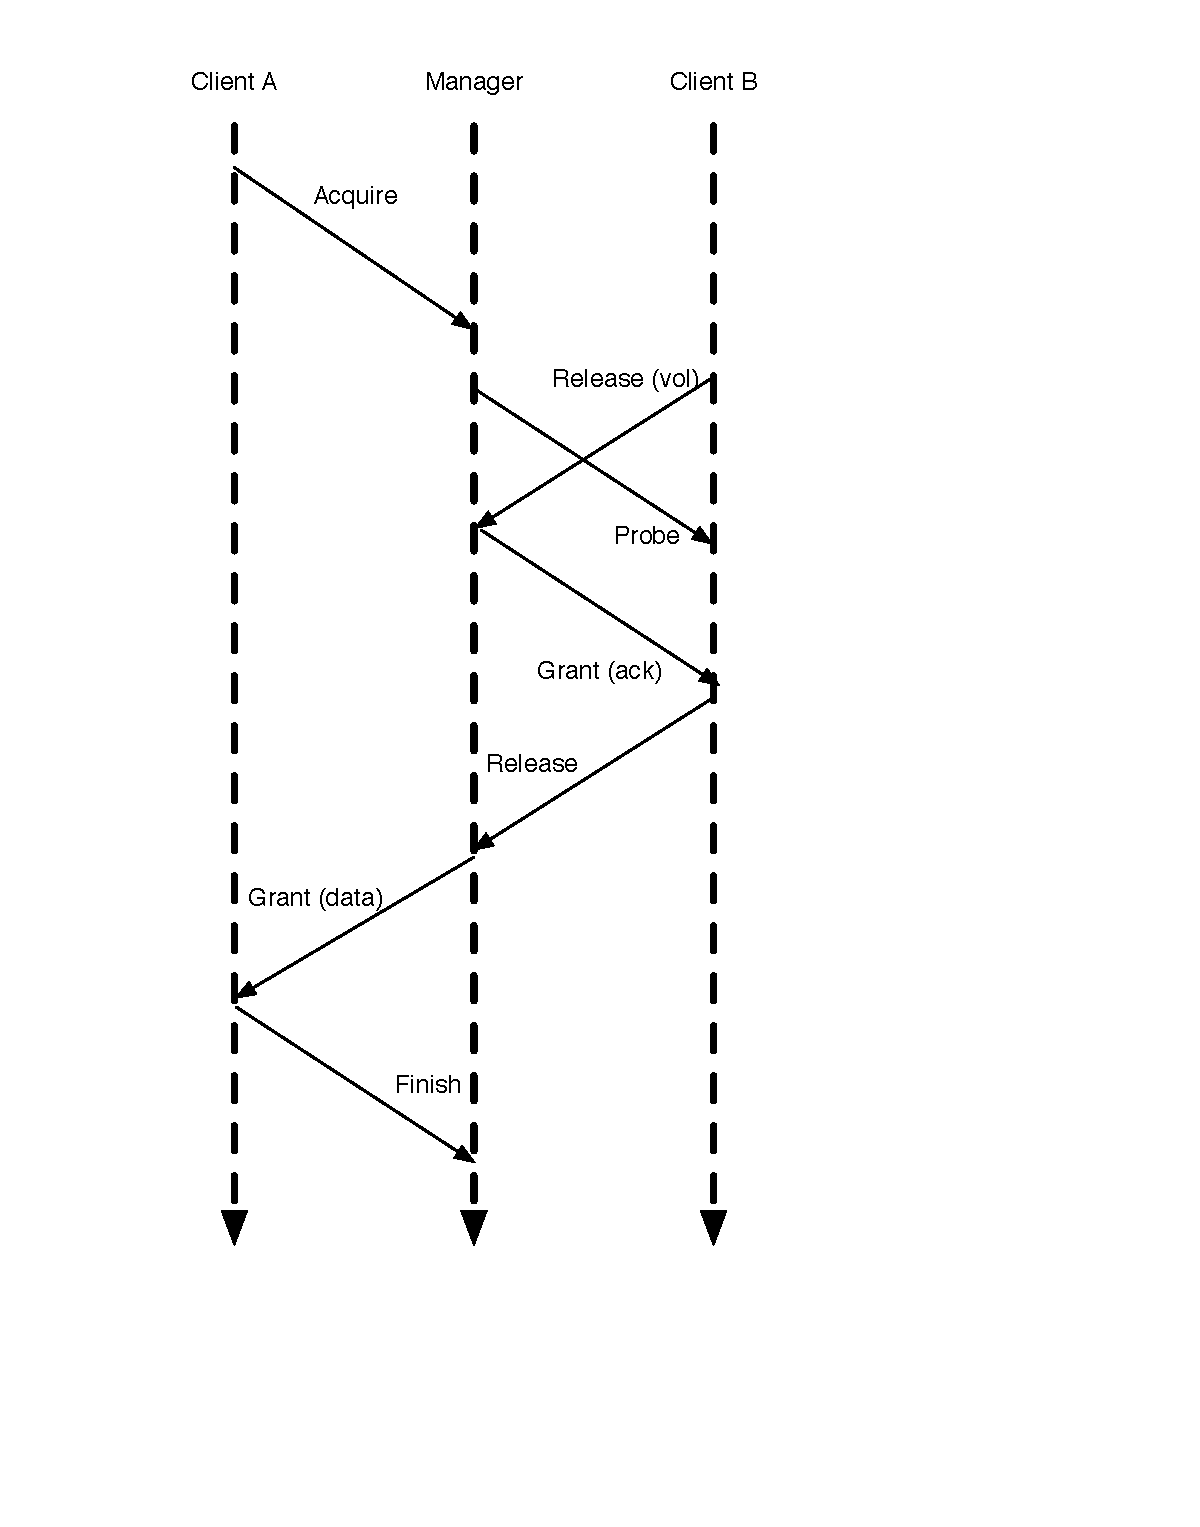
\includegraphics[width=0.5\columnwidth]{tilelink/figures/rel-merge.pdf}
\caption[Interleaved and well-ordered voluntary writeback message flows.]{
Interleaved message flows demonstrating acknowledgment Grants of voluntary writeback Releases.
Client A sends an Acquire to a manager, which then sends a Probe to Client B.
At the same time, Client B chooses to evict the same block and issues a voluntary Release.
The manager waits to receive a Release for every Probe that was sent, but additionally first accepts the voluntary Release.
The manager sends a special Grant that acknowledges receipt of the voluntary release.
Client B does not respond to the Probe until it gets the acknowledgment Grant.
Once Client B responds with a Release, Client A's transaction can proceed as normal.
}
\label{fig:rel-merge}
\end{figure}

We will first discuss the concurreny-limiting responsibility put on the manager.
The manager serves as a convenient point of synchronization across all the clients.
Since every transaction must be initiated via an Acquire message sent to a manager, the manager can trivially order the transactions.
A very safe implementation would be to accept only a single transaction's Acquire on a given cache block at a time,
but the performance implications of doing so are potentially dire, and it turns out we can be much more relaxed while continuing to provide a correct serialization.
Chapter~\ref{c:coherence} will provide an evaluation of the performance overheads of more limited TileLink concurrency.

At this time, TileLink forbids managers from accepting Acquires on the same cache block from different client sources.
Figure~\ref{fig:ordered} lays out this scenario in message sequence chart form.
Clients must continue to process and respond to Probes even with an outstanding Acquire pending in the network.
Managers must include an up-to-date copy of the data in Grants responding to Acquires upgrading permissions unless they are certain that that
client has not been Probed since the Aquire was issued.
Multiple acquires from the same source may be accepted, which we will discuss in more detail at the end of this section.
Assuming a manager has blocked on processing a second transaction Acquiring the same block, the critical question becomes: When is it safe for a manager to accept the pending Acquire?

If we were to assume point-to-point ordered delivery of messages over a particular channel,
it would be sufficient for the manager merely to have sent the Grant message to the original client source.
The manager could process further transactions on the block, and further Grants to the same client would arrive in order.
The act of updating the block's metadata and sending the Grant message is sufficient to serialize the transaction in the total ordering of transactions on the block.

However, TileLink intentionally does not make the point-to-point ordered delivery assumption.
Grants on the same block sent to the same client can arrive out of order.
Figure~\ref{fig:unordered} lays out this scenario in message sequence chart form.
Because Grants can arrive out of order, TileLink requires the addition of a final acknowledgment channel (Finish), which ensures that each Grant has been received by the client.
Note that some prior coherence protocols have addressed this particular complexity by blocking Probes until the Grant gets back to the source, but we will discuss why this solution can
cause deadlock in a hierarchical, nested system in the next section.

We now turn to the second concurrency-limiting responsibility, which is put on the client.
If a client has an outstanding voluntary writeback transaction on a block,
it cannot respond to an incoming Probe request on that block with Releases until it receives a Grant from the manager acknowledging completion of the writeback.
This limitation serializes the ordering of the voluntary writeback relative to the ongoing Acquire transaction.
The manager cannot simply block the voluntary release transaction until the Acquire transaction completes, because the Release message in that transaction will be
blocked behind the voluntary Release.
Figure~\ref{fig:rel-merge} lays out this scenario in message sequence chart form.

From the manager agent's perspective, it must handle the situation of receiving a voluntary Release for a block which another client is currently attempting to Acquire.
The manager must accept the voluntary Release as well as any Releases resulting from any Probe messages that have already been sent, and afterwards provide Grant messages to both clients before the transaction can be considered complete.
The voluntary write's data can be used to respond to the original requestor with a Grant, but the transaction cannot complete until the expected number of Releases
have been collected by the manager.
This scenario is an example of two transaction message flows being merged by the manager agent.

The final concurrency-limiting responsibility put on the client agent is to issue multiple Acquires for the same block only when the transactions can be differentiated from one another.
Typically, this differentiation takes the form of having different Acquire types or different transaction identifiers.
One possible case is for a client that has a write miss under a read miss to issue an Acquire asking for write permission before the Grant providing read permissions has arrived.
Managers are not obligated to accept both Acquires and merge the transactions' message flows, though they may choose to do so.
Further restrictions on issuing multiple Acquires to sub-block addresses via built-in transactions are detailed in Section~\ref{s.uncached}.


\subsection{Hierarchical TileLink}
\label{s.tlhier}

\begin{figure}[p]
\centering
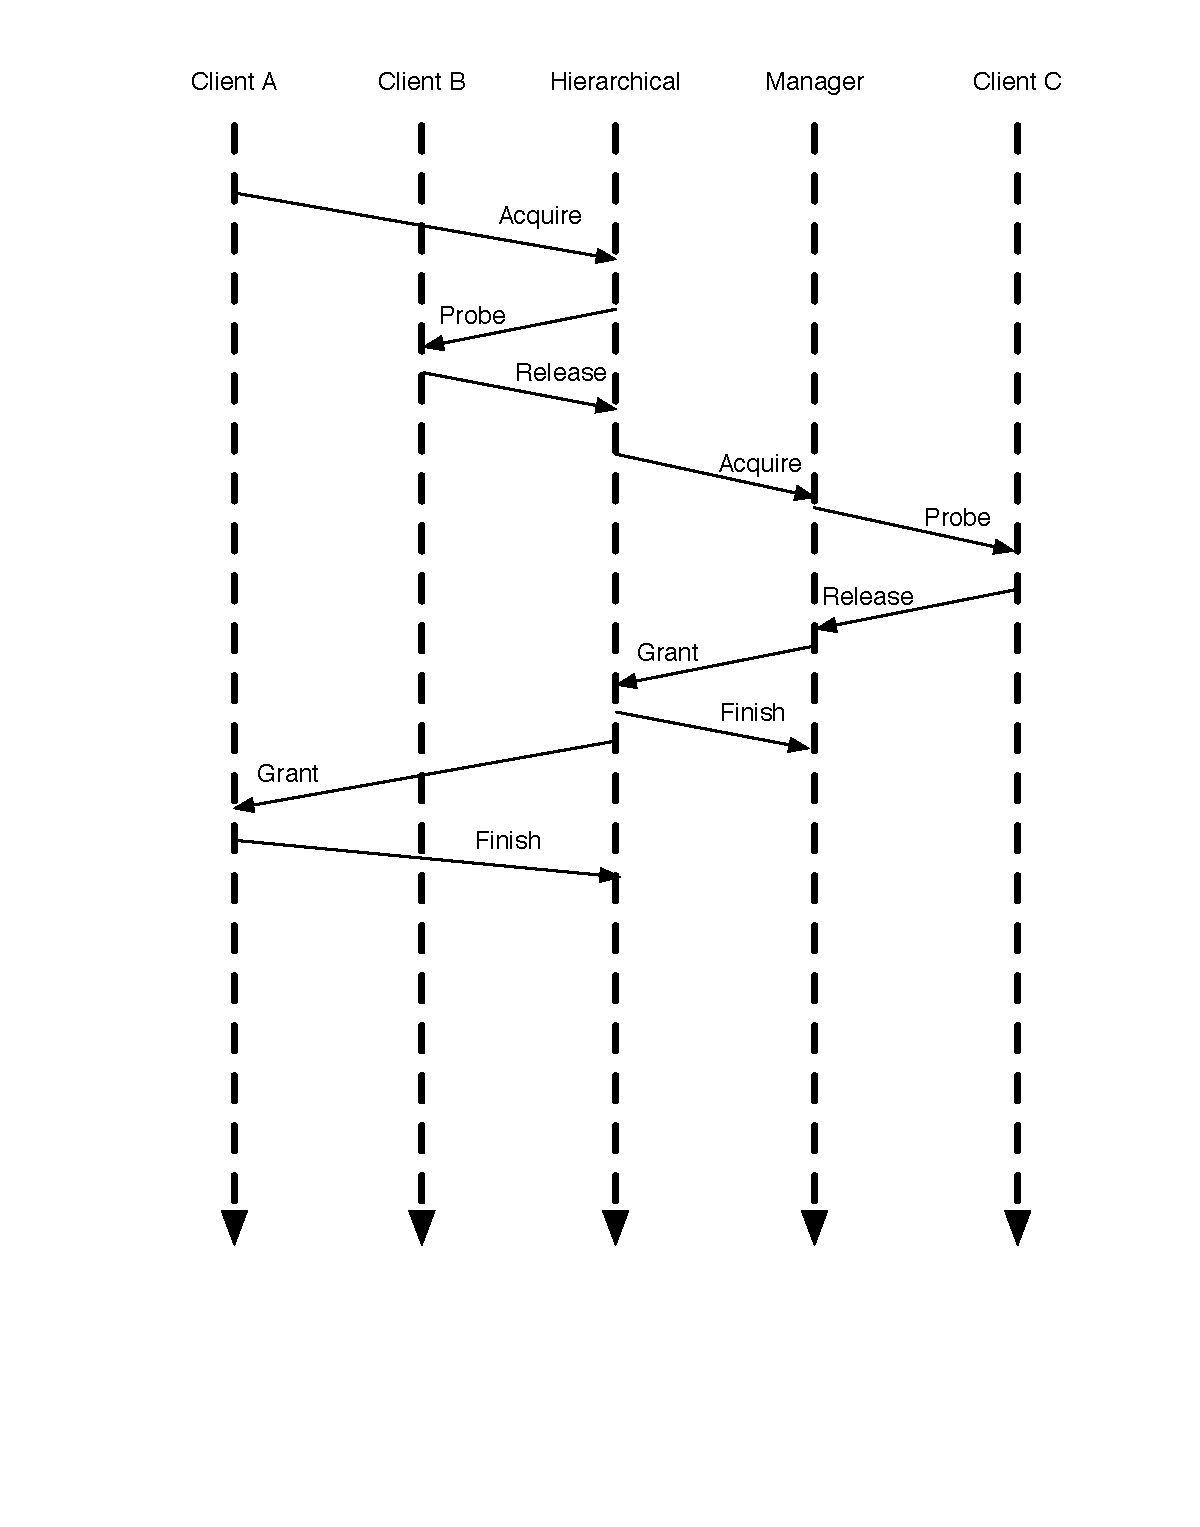
\includegraphics[width=0.8\columnwidth]{tilelink/figures/standard5.pdf}
\caption[A multi-level message flow.]{
Overview of a multi-level transaction's message flow.
After the hierarchical agent has Probed the clients under its purview, it falls back on initiating a transaction in the outer realm,
which is serviced by the outermost manager. Other branches of the memory hierarchy are Probed,
and any Released data is Granted back to the original source Client A by way of the hierarchical agent.
}
\label{fig:standard5}
\end{figure}

\begin{figure}[!p]
\centering
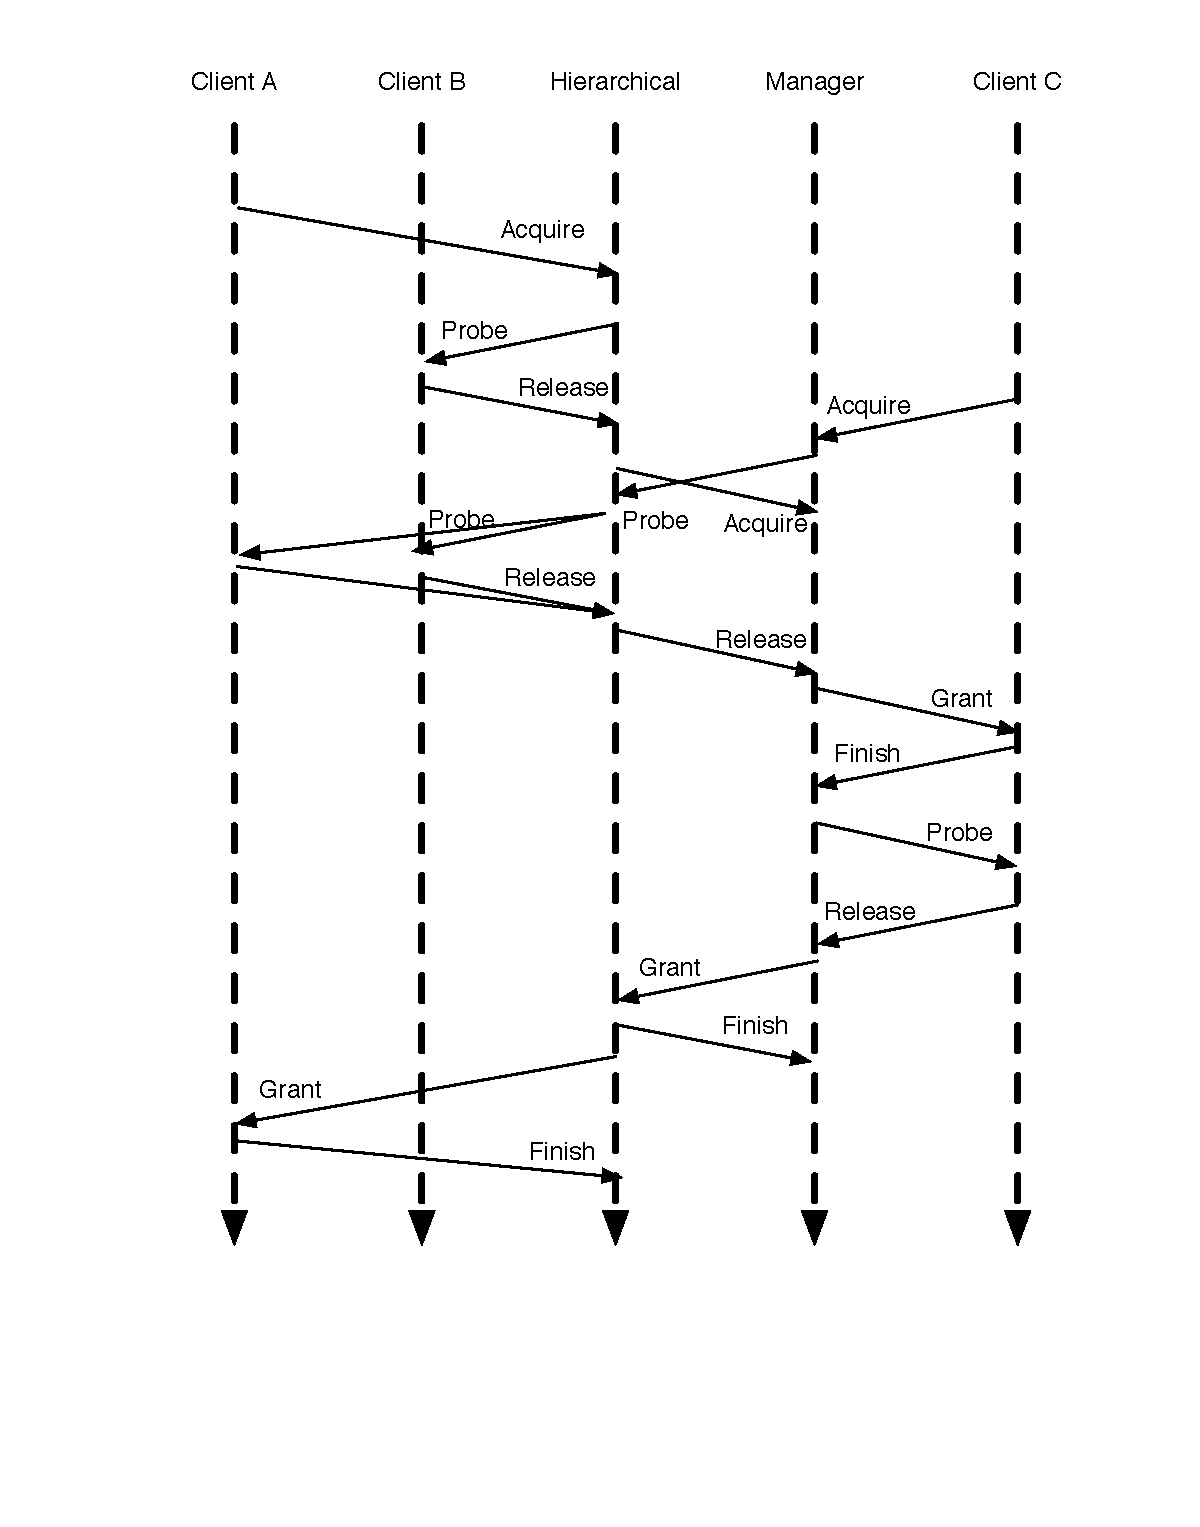
\includegraphics[width=0.8\columnwidth]{tilelink/figures/acq-merge-5.pdf}
\caption[A multi-level message flow including an Acquire race.]{
Overview of a multi-level transaction's message flow including an Acquire race.
Client A and Client C both issue Acquires. However, Client C's Acquire is the first to reach the outermost Manager, which means
it happens before Client A's transaction.
Client A must deal with Probes generated as part of Client C's transaction without deadlocking, even though it has already sent its own Acquire.
The Grant sent by the Hierarchical agent must take into account the fact that Client A was Probed mid-transaction.
}
\label{fig:acq-merge-5}
\end{figure}

\begin{figure}[!p]
\centering
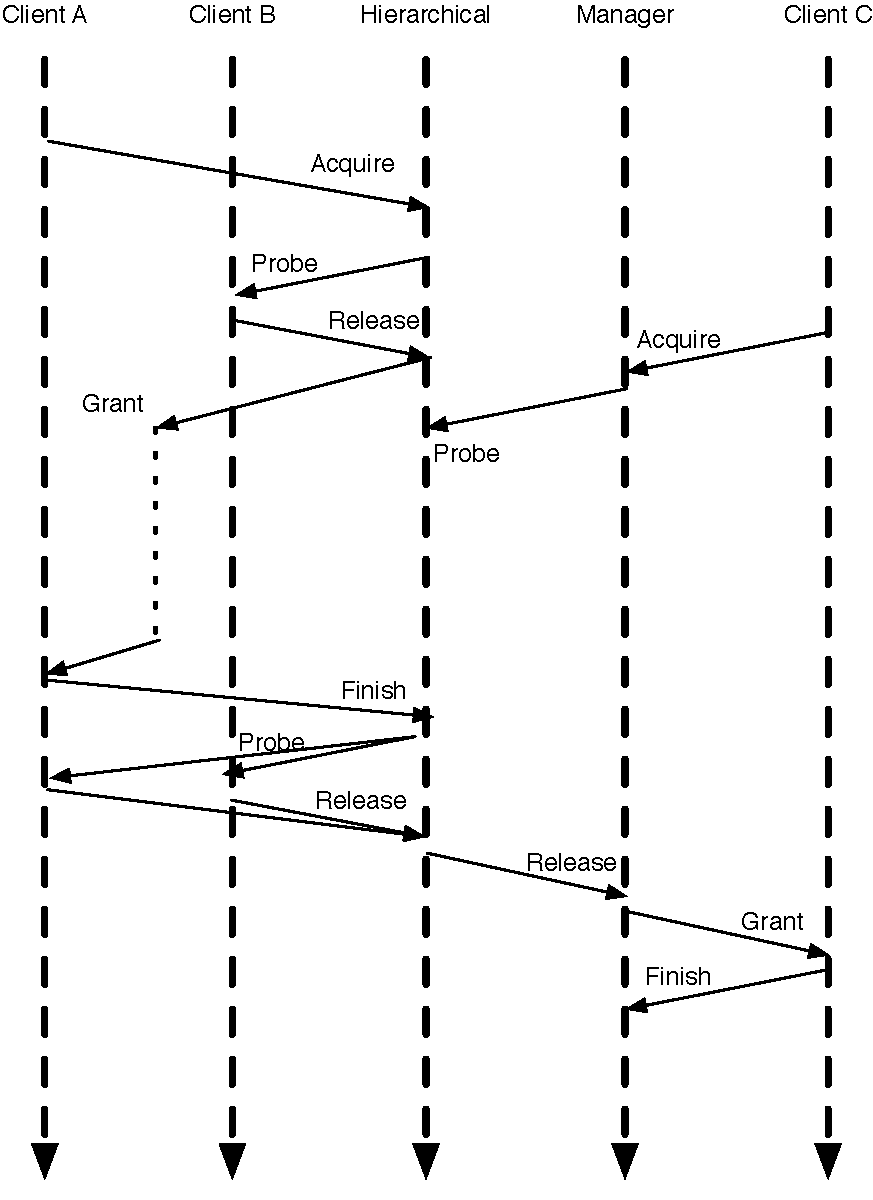
\includegraphics[width=0.8\columnwidth]{tilelink/figures/acq-merge-5-2.pdf}
\caption[Another multi-level message flow including an Acquire race.]{
Overview of a multi-level transaction's message flow including an Acquire race.
Client A and Client C both issue Acquires.
Client A's transaction is satisfiable locally, and a Grant is issued for it, which becomes delayed in the network.
Client C's Acquire is the first and only to reach the outermost Manager.
Client A must deal with Probes generated as part of Client C's transaction without deadlocking, even though it has already sent its own Acquire
and the Hierarchical agent has issued a Grant in response.
The Hierarchical Agent must wait until the Grant's Finish is received before forwarding the outer Probes inward.
}
\label{fig:acq-merge-5-2}
\end{figure}

TileLink is a hierarchical protocol that ascribes to the Manager-Client Pairing (MCP) architecture.
Each manager tracks and serializes transactions for all the clients within its coherence realm.
In situations where a manager does not have access or permissions on a particular piece of data,
it will in turn initiate a transaction in an outer realm.
Memory controllers at the root of the memory hierarchy are the ultimate managers, and they always have permission
to supply the data in the address range they control.

This structure results in nested sequences of messages, and we discuss some of the concurrency edge cases for these message flows here.
Details of how a transaction initiated in an inner realm is translated into the protocol of the outer realm are left to the next chapter.
Figure~\ref{fig:standard5} lays out a basic multi-level transaction in message sequence chart form.
The transaction between the hierarchical agent and the outermost manager is nested within the inner transaction.
The outer Acquire is sent based on the inner Acquire. 
The inner Grant is dependent on the outer Grant response.
Probes may be launched into other branches of the memory hierarchy.

Figures~\ref{fig:acq-merge-5}~and~\ref{fig:acq-merge-5-2} lay out concurrency races between two multi-level transactions in message sequence chart form.
The transaction whose Acquire is first to reach the outermost Manager required to gain sufficient permissions 
\emph{happens~before} the other transaction.
The final state of the data and permissions in the system must reflect this ordering
in order for their to be a global serialization of the transactions on the block.

The transaction that won the race in the outer level may issue Probes into the branch of the memory hierarchy where the other transaction has begun to be processed.
These Probes must be responded to with Releases to prevent deadlock in the outer level.
However, this means that the inner transaction and outer transaction must be merged successfully.
If the inner transaction has not yet sent a Grant to the originator (Figure~\ref{fig:acq-merge-5}),
the Grant sent must take into account the fact that Client A was Probed mid-transaction.
If the inner transaction has already sent a Grant to the originator (Figure~\ref{fig:acq-merge-5-2}),
then the outer Probes must not be forwarded until the receipt of the Grant is acknowledged with a Finish message from the original client.

\section{Built-in Transactions}
\label{s.uncached}

One of the design goals of TileLink was to support heterogeneous SoC designs that consist of a wide variety of agents.
In particular, we wanted to support accelerators that operate on the same global shared memory space as the general-purpose cores, possibly at very high bandwidths.
However, while these accelerators need a coherent view of memory, they do not necessarily cache copies of data themselves.
We wanted cacheless accerators to be able to interoperate with any coherence policy implemented on top of the TileLink protocol, without having to know anything about coherence policies internally.

These design goals led us to create a set of {\em built-in} transactions available to any client connected to a TileLink substrate.
We provide seven built-in transaction types that are available to all clients that want to participate in the coherence protocol, even if they themselves will not keep cached copies of the data.
Because these transactions do not create a new private copy of the targeted cache block, we term them ``uncached'' transactions. 
However, they still participate in the standard TileLink transaction flow, meaning that they will result in probes of other caches and return coherent answers.

\subsection{Built-in Transaction Types}

The uncached transactions available to all TileLink clients are as follows:
\begin{description}
\item[Get:] Fetches a single beat of data from a cache block and returns only that beat.
\item[GetBlock:] Fetches an entire cache block and serves it back to the requestor.
\item[GetPrefetch:]  Prefetches a cache block into the next-outermost level of the memory hierarchy with read permissions.
\item[Put:] Writes up to a beat's worth of data to backing memory. Uses a write mask to determine which bytes contain valid write data.
\item[PutBlock:] Writes out an entire cache block to backing memory.
\item[PutPrefetch:]  Prefetches a cache block into the next-outermost level of the memory hierarchy with write permissions.
\item[PutAtomic:] Performs an atomic memory op in the next-outermost level of the memory hierarchy. The maximum available operand size is 64b (sizes and opcodes per RISC-V atomic instructions).
\end{description}

There are five built-in types of Grant that are available to all managers that want to participate in the coherence protocol.
Because ``uncached'' transactions do not create a new private copy of the targeted cache block, we use these Grant types mostly as acknowledgments.
The available types are as follows:
\begin{description}
\item[GetDataBlock:] Full cache block in response to Acquire.GetBlock.
\item[GetDataBeat:] Single beat of data in response to Acquire.Get or Acquire.PutAtomic.
\item[PutAck:] Acknowledgement of Acquire.\{Put, PutBlock\}.
\item[PrefetchAck:] Acknowledgment of Acquire.\{GetPrefetch, PutPrefetch\}.
\item[VoluntaryAck:] Acknowledgement of any voluntary Release.
\end{description}

The PutBlock message is unique among the built-in Acquire types in that it contains multiple beats of data (if the cache block size is larger than the parameter {\tt TLDataBits}).
The client controller that generates this message is responsible for generating multiple sequential PutBlock messages and incrementing the {\tt addr\_beat} field as it does so.
The GetDataBlock message also contains multiple beats of data (again, if the cache block size is larger than {\tt TLDataBits}).
The manager controller that generates this message is responsible for generating multiple sequential GetDataBlockmessages and incrementing the {\tt addr\_beat} field as it does so.
In contrast, a GetDataBeat message only ever consists of a single beat.
A single VoluntaryAck is used to respond to each voluntary Release, even if that Release consists of multiple beats.
Similarly, a single PutAck is used to respond to a PutBlock message containing multiple beats.

\begin{table}[ht]
\begin{center}
\begin{tabular}{|l|l|l|}
    \hline
    Acquire & Grant & Effect \\ \hline \hline
    Get & GetDataBeat & Copy data in to client \\ \hline
    GetBlock & GetDataBlock & Copy data in to client \\ \hline
    GetPrefetch & PrefetchAck & Fetch data to outer memory with read permissions \\ \hline
    Put & PutAck & Update data in outer memory \\ \hline
    PutBlock & PutAck & Update data in outer memory \\ \hline
    PutPrefetch & PrefetchAck & Fetch data to outer memory with write permissions \\ \hline
    PutAtomic & GetDataBeat & Update data in outer memory and return old value. \\ \hline
\end{tabular}
\end{center}
\caption[Overview of built-in, uncached transactions.]{
Overview of built-in, uncached transactions. Each type of Acquire results in a particular acknowledgment or data Grant.}
\label{tab:uncached}
\end{table}

Table~\ref{tab:uncached} provides and overview of the built-in transactions and their effect on memory.
In a hierarchical system, uncached transactions may be turned into cached transactions in outer levels of the memory hierarchy.
We provide an allocation flag on the Acquire messages to govern whether this conversion is allowed.

Whether an address is cached or uncached is a property of the transaction, not the address. Certain clients may cache an address, while other clients at the same level may not. If the allocation flag is set to true, a hierarchical agent may choose to convert an uncached transaction into a cached one, which will result in the data becoming cached at the outer level. It will still not be cached by the original requestor (who asked for it uncached). If the allocation flag is false, the hierarchical agent must also issue the transaction uncached and merely forward the grant back to the original requestor without caching the data locally.
 
\subsection{Memory Model for Built-In Sub-Block Transactions}

TileLink is intended to be compatible with the weak memory consistency model adopted by the RISC-V ISA, and its design will not impose any performance overhead on any similarly weak model.
Specifically, TileLink channels are not required to perform in-order delivery of messages, and hierarchical and manager agents are not required to process transactions in a particular order.
Therefore, client agents are responsible for enforcing orderings between memory operations by
waiting to initiate new transactions until all relevant outstanding transactions have been completed.
Uncached transactions that do not return data to the client still receive
acknowledgments of operation completion from the manager,
which allows for clients to make decisions about when to issue further requests.
This division of labor means that TileLink can support stronger memory models,
such as Sequential Consistency, by placing the burden of enforcing the
stronger model on the agents that are issuing the memory operations.
It is worth noting that even in a system with a weak memory model, 
clients should always avoid issuing multiple requests to any particular address at the same time,
as the Acquire messages may be reordered, resulting in non-sequential memory operation orderings
to a single address.

\subsection{Concurrency for Built-In Sub-Block Transactions}

\begin{figure}[p]
\centering
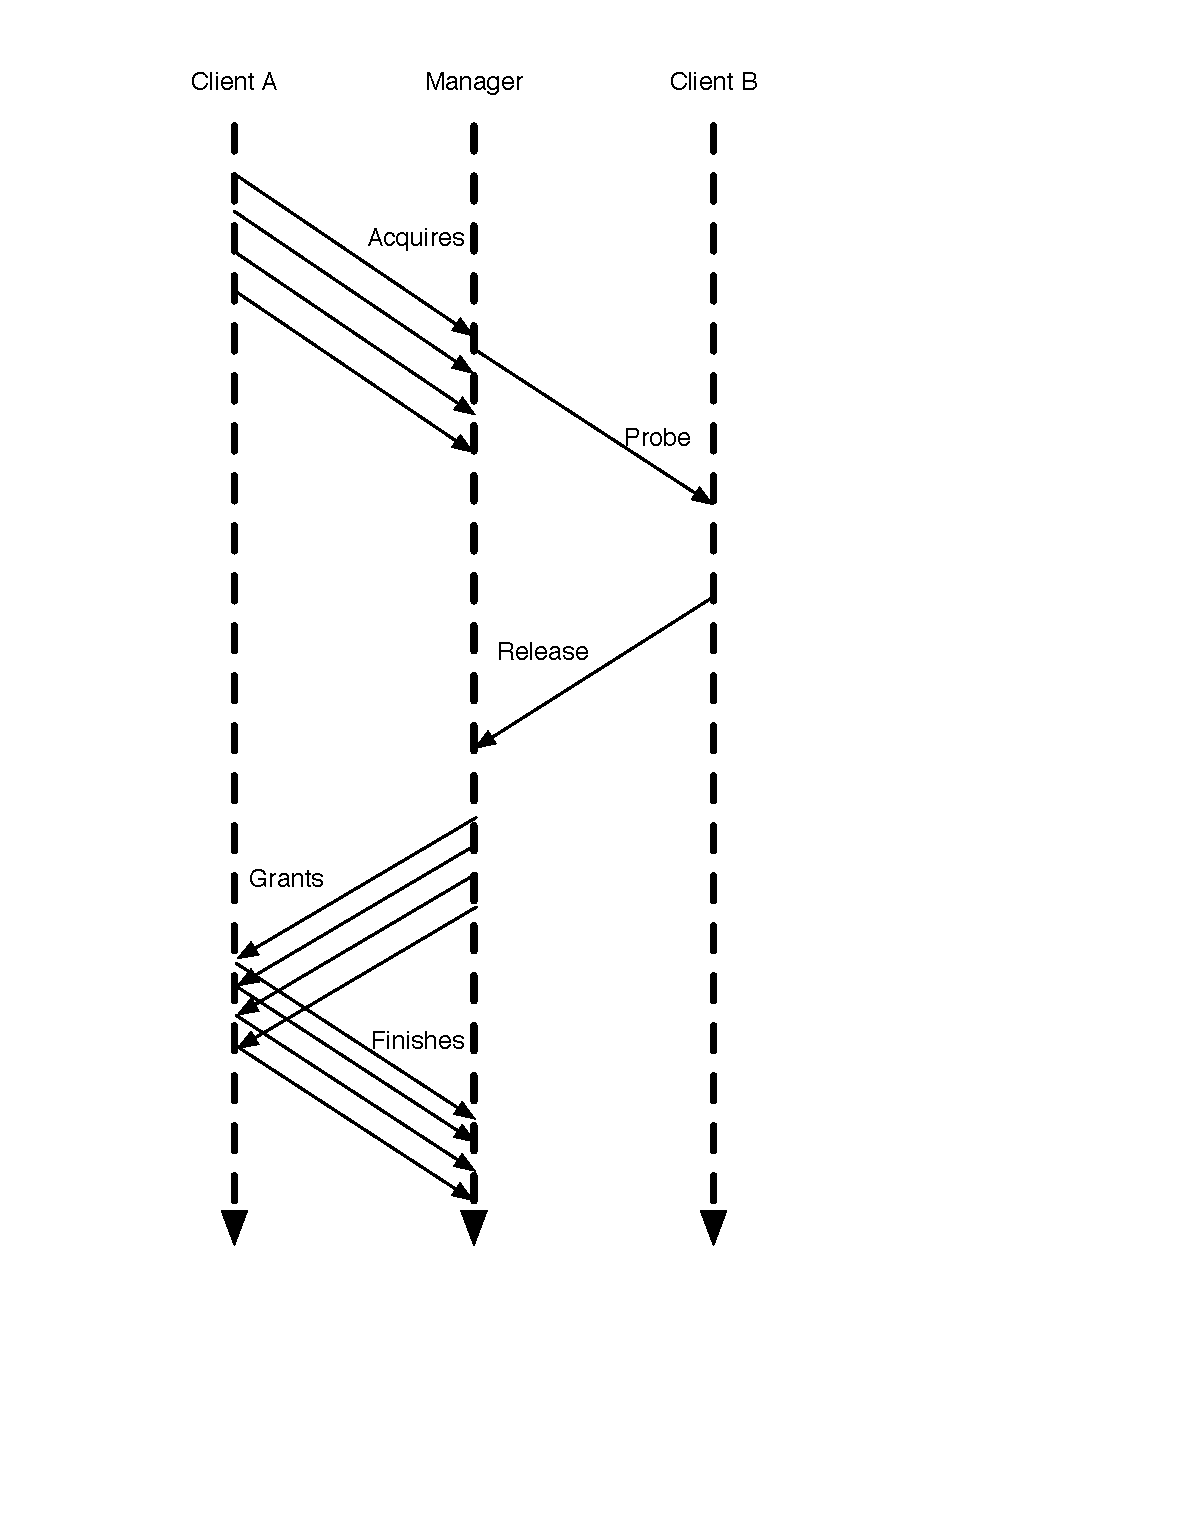
\includegraphics[width=0.5\columnwidth]{tilelink/figures/acq-merge.pdf}
\caption[Interleaved message flows merging multiple ``uncached'' transactions.]{
Interleaved message flows demonstrating merging of multiple ``uncached'' transactions from the same client.
As long as the Acquires target different sub-block addresses they are safe to interleave.
Multiple Grants and Finishes can also be in flight simultaneously, and the transaction terminates when the correct count of Finishes is accepted.}
\label{fig:acq-merge}
\end{figure}

In order to support high-bandwidth access to cached data blocks from data-parallel accelerators, TileLink enables many outstanding built-in, sub-block transactions
to be in flight in the memory hierarchy at once.
In general, it is preferable to merge such transactions on the client side, before they are even exposed to the TileLink interface.
However, in order to provide support for secondary misses in hierarchical agents, we define the following rules for transaction merging.

As long as the Acquires used to initiate the transaction target different sub-block addresses, it is safe to interleave their processing by merging the transactions with one another.
The Acquires must be attempting to gain the same permissions and perform the same operation.
They must also have unique transaction identifiers.
Acquires from multiple client agents can be merged so long as they meet the above requirements.

Figure~\ref{fig:acq-merge} illustrates a merging scenario from a single client.
Multiple Grants and Finishes can also be in flight simultaneously, and the overall merged transaction terminates when the correct count of Finishes is accepted.
In order to prevent starvation of other clients, merging secondary sub-block transactions should not be prioritized over processing transactions initiated by other clients.
Merging transactions is an allowable performance optimization, not a requirement.

\section{Assumptions and Guarantees}

As we move towards a formal specification of TileLink, an important step is to provide a set of invariants to which any implementation must conform.
If any of these assumptions are not met by a particular implementation of physical network, client agent,
or manager agent, then the system can either deadlock or produce an incoherent view of global shared memory.
Conversely, composing a set of implementations that meet all these assumptions will
guarantee a deadlock-free implementation of cache coherency.
The following list collects the requirements necessary for a correct TileLink implementation:
\begin{itemize}
\item If a message contains multiple beats of data, all beats will eventually be sent.
\item A client issuing an Acquire will eventually receive a corresponding Grant.
\item A client receiving a Grant will issue a corresponding Finish,
unless the physical network is known to provide in-order delivery.
\item A client receiving a Probe will issue a corresponding Release.
\item A client issuing a voluntary Release will receive a corresponding Grant (of type VoluntaryAck), 
unless the physical network is known to provide in-order delivery.
\item Managers always consume any available Finish messages.
\item No duplicate messages will be created by any agents or within any channels.
\item All messages will eventually be delivered by the physical channels; a message cannot be lost.
\item No Finish is ever blocked by another message type.
\item Grants may only be blocked by Finishes.
\item Releases may only be blocked by Finishes and Grants.
\item Probes may only be blocked by Finishes, Grants, and Releases.
\item If a client has an outstanding voluntary Release on a block, it will not respond to a Probe on that block until it receives the Release's corresponding acknowledgment Grant.
\item If a client has an outstanding voluntary Release on a block, it will not issue an Acquire on that block until it receives the Release's corresponding Grant.VoluntaryAck.
\item If a manager has already has accepted an Acquire on a block, it will not issue Probes or Grants in response to a second Acquire on that block until it receives a Finish from the first Acquire's source.
\item A manager will always include a copy of the data in a Grant, unless it can prove that the client had a copy of the block when the Acquire was accepted and no Probes from outer memory for that block have been received.
\item Clients may not issue multiple Acquires with the same {\tt client\_xact\_id} and {\tt addr\_block} fields, unless they have different {addr\_beat}, {a\_type}, or {union} fields.
\item A Hierarchical agent will block Probes from being forwarded from its outer client interface to its inner manager interface until it has received Finishes for all Grants on that block.
\end{itemize}

\section{Channel Signal Descriptions}
\label{s.types}

This section details the specific signals contained in each channel of the TileLink protocol.
Every channel is wrapped in a decoupled interface, meaning that each contains ready and valid signals as well as the following bundles of signals.
Channels whose message types may contain data (i.e., Acquires, Releases and Grants) may send the data over multiple beats
if the cache block size is larger than \code{TLDataBits}.
The agent controller that generates these multi-beat messages is responsible for generating the correct number of sequential beat messages and incrementing the \code{addr\_beat} field as it does so.
Tracking beat counts in this way exposes the width of the underlying network to the controllers, 
but we propose that this encapsulation deficiency is necessary in order to improve the efficiency of refilling data into caches whose data array rows are of a matching size to the physical network.


%\subsection{Acquire}

\emph{Acquires} initiate a transaction to acquire access to a cache block with proper permissions for a particular memory operation.
Acquires are also used to write data into outer memory (acquiring permissions for the write as it does so), perform an atomic operation in outer memory, or prefetch data with particular permissions.
Table~\ref{tab:acquire} shows all the fields of the Acquire channel.
Some of the fields used for certain built-in transactions are multiplexed onto the Union field.
Table~\ref{tab:union} shows all these sub-fields and indicates which are used for each type
of built-in Acquire message.

\begin{table}[p]
\begin{center}
\begin{tabular}{|l|l|l|}
    \hline
    Name & Type & Purpose \\ \hline \hline
addr\_block & UInt & Physical address of the cache block, with block offset removed \\ \hline
client\_xact\_id & UInt & Client's id for the transaction \\ \hline
data & UInt & Client-sent data, used for Put transactions \\ \hline
addr\_beat & UInt & Offset of this beat's worth of data within the cache block \\ \hline
built\_in\_type & Bool & Whether the transaction is a built-in or custom type \\ \hline
a\_type & UInt & Type of the transaction. For built-in transactions, one of: \\
        &      & \{Get, GetBlock, GetPrefetch, Put, PutBlock, PutPrefetch, PutAtomic\}, \\
        &      &  Otherwise defined by the coherence protocol \\ \hline
union & Union & Used to derive and derive the sub-fields in Table~\ref{tab:union} \\ \hline
\end{tabular}
\end{center}
\caption{Fields of the Acquire channel.}
\label{tab:acquire}
\end{table}

\begin{table}
\begin{center}
\begin{tabular}{|l|l|c|c|c|c|l|}
    \hline
Name       & Type & Get & Put & Atomic & Prefetch & Purpose \\ \hline \hline
allocate   & Bool & X   & X   &        &          & Hints whether to allocate data in outer caches \\
           &      &     &     &        &          & when servicing this request \\ \hline
op\_code   & UInt & X   & X   & X      & X        & Memory op code; see Appendix~\ref{a.memopcodes}) \\ \hline
op\_size   & UInt &     &     & X      &          & Size of the AMO operands (b/h/w/d) \\ \hline
addr\_byte & UInt & X   &     & X      &          & Address of the word within the block \\ \hline
wmask      & UInt &     & X   &        &          & Byte write mask for Put data \\ \hline
\end{tabular}
\end{center}
\caption[The union field of the Acquire channel.]{
Input sub-fields used to fill in the Union field of the Acquire channel for built-in messages.
`X' indicates which  subfields are meaningful for which built-in message types.
}
\label{tab:union}
\end{table}


%\subsection{Probe}

\emph{Probes} query a client to determine whether it has a cache block or to revoke that client's  permissions on that cache block.
Table~\ref{tab:probe} shows all the fields of the Probe channel.

\begin{table}[]
\begin{center}
\begin{tabular}{|l|l|l|}
    \hline
    Name & Type & Purpose \\ \hline \hline
addr\_block & UInt & Physical address of the cache block, with block offset removed \\ \hline
p\_type & UInt & Transaction type, defined by coherence protocol \\ \hline
\end{tabular}
\end{center}
\caption{Fields of the Probe channel.}
\label{tab:probe}
\end{table}


%\subsection{Release}

\emph{Releases} provide an acknowledgment of Probe receipt by clients, releasing certain permissions on the block along with any dirty data back to the manager.
Releases are also used by clients to voluntarily write back data or cede permissions on the block.
Table~\ref{tab:release} shows all the fields of the Release channel.

%Release messages may contain multiple beats of data (if the cache block size is larger than TLDataBits).
%The client controller that generates this message is responsible for generating multiple sequential Release messages and incrementing the \code{addr\_beat} field as it does so.

\begin{table}[]
\begin{center}
\begin{tabular}{|l|l|l|}
    \hline
    Name & Type & Purpose \\ \hline \hline
addr\_block & UInt & Physical address of the cache block, with block offset removed \\ \hline
client\_xact\_id & UInt & Client's id for the transaction \\ \hline
data & UInt & Used to writeback dirty data \\ \hline
addr\_beat & UInt & Offset of this beat's worth of data within the cache block \\ \hline
r\_type & UInt & Transaction type, defined by coherence protocol \\ \hline
voluntary & Bool & Whether this release is voluntary or in response to a Probe \\ \hline
\end{tabular}
\end{center}
\caption{Fields of the Release channel.}
\label{tab:release}
\end{table}

%\subsection{Grant}

\emph{Grants} provide data or permissions to the original requesting client, granting it access to the cache block.
Grants are also used to acknowledge voluntary Releases.
Table~\ref{tab:grant} shows all the fields of the Grant channel.

%The GetDataBlock message may contain multiple beats of data (if the cache block size is larger than TLDataBits).
%The manager controller that generates this message is responsible for generating multiple sequential
%GetDataBlock messages and incrementing the \code{addr\_beat} field as it does so.

\begin{table}[]
\begin{center}
\begin{tabular}{|l|l|l|}
    \hline
    Name & Type & Purpose \\ \hline \hline
built\_in\_type & Bool & Whether transaction type is built-in or custom \\ \hline
g\_type & UInt & Type of the transaction. For built-in transactions, one of: \\
        &      & \{VoluntaryAck, PrefetchAck, PutAck, GetDataBeat, GetDataBlock\}. \\
        &      & Otherwise defined by the coherence protocol \\ \hline
client\_xact\_id & UInt & Client's id for the transaction \\ \hline
manager\_xact\_id & UInt & Manager's id for the transaction, passed to Finish \\ \hline
data & UInt & Used to supply data to original requestor \\ \hline
addr\_beat & UInt & Offset of this beat's worth of data within the cache block \\ \hline
\end{tabular}
\end{center}
\caption{Fields of the Grant channel.}
\label{tab:grant}
\end{table}


%\subsection{Finish}

\emph{Finishes} provide a final acknowledgment of transaction completion from requestor and are used to preserve transaction ordering.
Table~\ref{tab:finish} shows all the fields of the Finish channel.

\begin{table}[]
\begin{center}
\begin{tabular}{|l|l|l|}
    \hline
    Name & Type & Purpose \\ \hline \hline
manager\_xact\_id & UInt & Manager's id for the transaction \\ \hline
\end{tabular}
\end{center}
\caption{Fields of the Finish channel.}
\label{tab:finish}
\end{table}

\section{Agent-Specific Views of Logical TileLink Networks}

\begin{figure}[p]
\centering
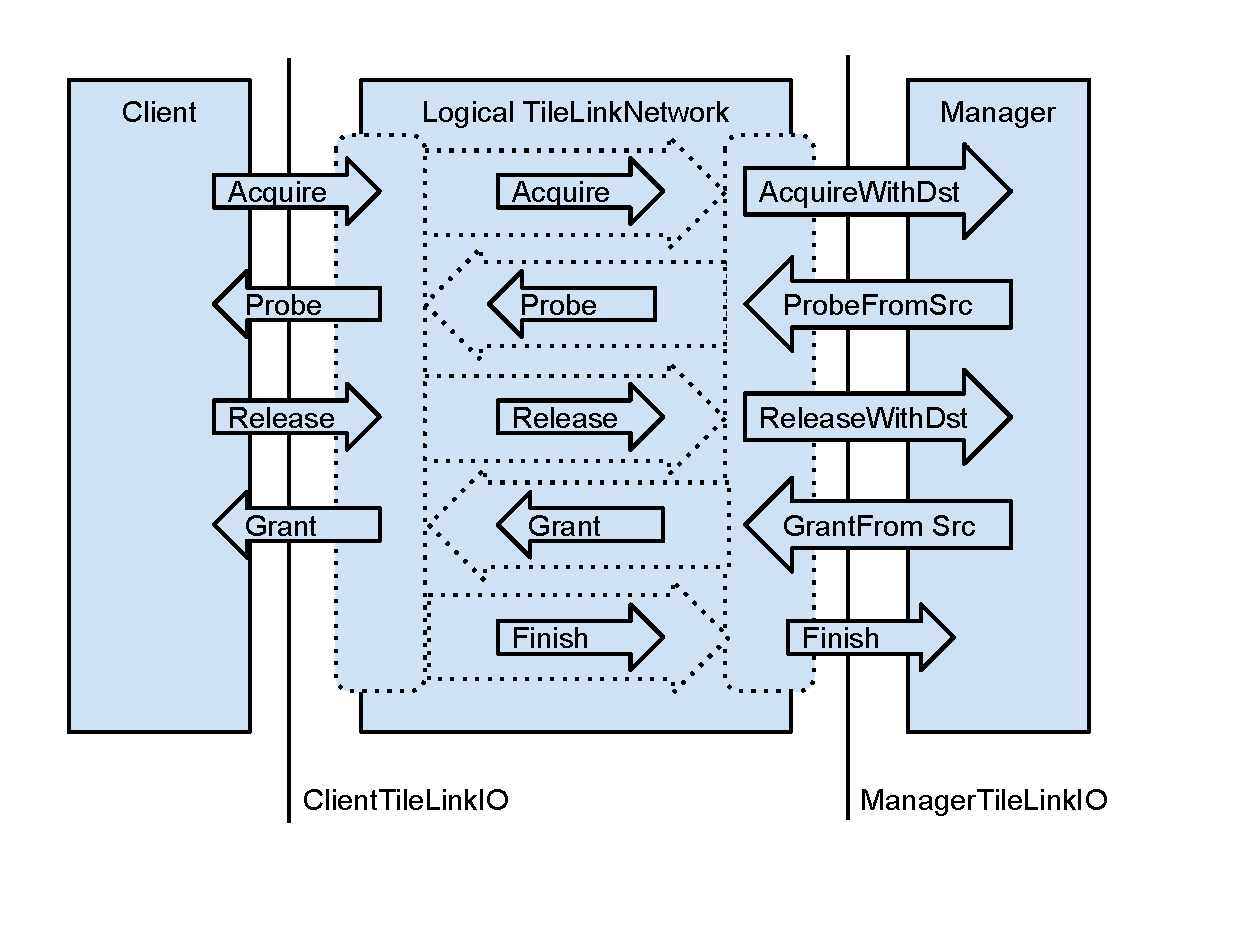
\includegraphics[width=1\columnwidth]{tilelink/figures/agent-specific.pdf}
\caption[Agent-specific views of TileLink.]{Overview of the logical view of the TileLink interface presented to each type of agent.}
\label{fig:agent}
\end{figure}

For the convenience of designers implementing Client and Manager agents, we provide TileLinkNetworkPort modules which abstract away the details of the on-chip network implementation.
These network ports automatically generate networking headers, perform serialization/deserialization for narrower physical network channels, and generate appropriate control flow logic.
The ports then expose simplified subsets of the TileLink channels to the agent modules.
Figure~\ref{fig:agent} provides an overview of these two interfaces.

{\em ClientTileLinkIO} consists of standard Acquire, Probe, Release, and Grant message channels.
It does not include the Finish channel as generating those acknowledgments is handled by the ClientTileLinkNetworkPort.

{\em ManagerTileLinkIO} consists of Acquire, Probe, Release, and Grant message channels that have additional data appended about the source or destination of messages, expressed in terms of the client and managers' network identifiers.
Acquires and Releases include their source id, and Probes and Grants are supplied a destination id.
The Client id format and numbering is determined by the characteristics of the physical network and is encapsulated from TileLink.
This interface does include a Finish channel so that the manager knows when to register the transaction as complete.

Clients and managers may share a network port of the associated type as long as their pools of transaction identifiers are unique.
In practice, we often support this requirement by utilizing routers that automatically prepend bits to the \code{client\_xact\_id} field
for outgoing messages, while using the same bits to route incoming messages.
This capability is useful for multiplexing ports in cases where the width of the interface is constrained.

\section{TileLink Parameters}
\label{s.tlparam}

This section defines a set of parameters that are exposed by the TileLink to the top-level design.
Table~\ref{tab:tlparams} provides an overview of the available parameters.
The majority are used to determine the widths of the various channels fields that we have previously discussed.

\begin{table}[t]
\begin{center}
\begin{tabular}{|l|l|l|}
    \hline
Name & Type & Function \\ \hline \hline
TLId & String & Ids a TileLink in a multi-level hierarchy \\ \hline
TLCoherencePolicy & CoherencePolicy & Coherency policy used on this TileLink \\ \hline
TLNManagers & Int & Number of manager agents \\ \hline
TLNClients & Int & Number of client agents \\ \hline
TLNCachingClients & Int & Number of client agents that cache data \\ \hline
TLNCachelessClients & Int & Number of client agents that do not cache data \\ \hline
TLMaxClientXacts & Int & Max number of concurrent transactions per client \\ \hline
TLMaxClientsPerPort & Int & Max number of clients sharing a single network port \\ \hline
TLMaxManagerXacts & Int & Max number of concurrent transactions per manager \\ \hline
TLBlockAddrBits & Int & Address size \\ \hline
TLDataBits & Int & Amount of block data sent per beat, must be >= XLEN \\ \hline
TLDataBeats & Int & Number of beats per cache block \\ \hline
%TLNetworkIsOrderedP2P & Boolean & Whether the underlying physical network \\
%                      &         & preserved point-to-point ordering of messages \\ \hline
\end{tabular}
\end{center}
\caption[Independent parameters of TileLink.]{
Exposed top-level TileLink independent parameters.
These can be set uniquely for each realm of the memory hierarchy.}
\label{tab:tlparams}
\end{table}

We use the Context Dependent Environments described in Chapter~\ref{c.parameters} to define and supply these values
at each level of the memory hierarchy during the hardware elaboration process.
Presently, we encode all parameters with a single Scala case class, and then supply an instance of that class in
response to query points within the Chisel \code{Module} and \code{Bundle} classes that serve as Tilelink endpoints or channels.
Each case class corresponds to a single TileLink realm.
We also provide a geographical \code{TileLinkKey} that external generators can use to specialize heterogeneous TileLink
networks when multiple networks are instantiated within a given chip, by providing a different case class for each realm.

Figure~\ref{fig:tlgeo} outlines a sketch of how we can provide multiple configurations of TileLink to an individual Module using CDEs.
The trick is to recursively use two Parameters objects to disambiguate the inner and outer TileLink channel width parameters.
These parameters can be bound to specific instances of TileLinkParameters defined in the top-level definitions.
The recursive use of Parameters here allows for another level of indirection, which in turn allows each agent
in a hierarchical tree of agents to be specialized according to the parameters of its inner and outer network.
The code inside of the agents refers to them purely in terms of ``inner'' and ``outer,'' without
requiring any further knowledge of where this level exists in the global hierarchy.
A set of parameters that is ``inner'' for one manager agent can be assigned to be the ``outer'' parameters of`its clients.
This encapsulation of geographical information and indirection based on nested parameter values would not be possible without
the capabilities afforded us by deploying CDEs.

\begin{figure}
\centering
\begin{scala}
case class TileLinkParameters(
    coherencePolicy: CoherencePolicy,
    nManagers: Int,
    nClients: Int,
    dataBits: Int,
    dataBeats: Int = 4,
    overrideDataBitsPerBeat: Option[Int] = None
    ) {
  val writeMaskBits: Int  = ((dataBits / dataBeats) - 1) / 8 + 1
  val dataBitsPerBeat: Int = overrideDataBitsPerBeat.getOrElse(dataBits / dataBeats)
}

case object TLKey extends Field[TileLinkParameters]
case object InnerTLId extends Field[String]
case object OuterTLId extends Field[String]

trait HasCoherenceAgentParameters {
  implicit val p: Parameters
  val outerTLId = p(OuterTLId)
  val outerTLParams = p(TLKey(outerTLId))
  val outerDataBeats = outerTLParams.dataBeats
  ...
  val innerTLId = p(InnerTLId)
  val innerTLParams = p(TLKey(innerTLId))
  val innerDataBeats = innerTLParams.dataBeats
}

class DefaultConfig extends Config (
  topDefinitions = { (pname,site,here) =>
    ...
      case BuildL2CoherenceManager => (id: Int, p: Parameters) =>
        Module(new L2BroadcastHub()(p.alterPartial({
          case InnerTLId => "L1toL2"
          case OuterTLId => "L2toMC" })))
      case TLKey("L2toMC") =>
        TileLinkParameters(
          coherencePolicy = new MEICoherence(...)
          nCachingClients = site(NBanksPerMemoryChannel), ...)
      ...
})

\end{scala} 
\caption[Using recursive parameters to encapsulate geographic TileLink parameters.]{
An example of using recursive parameters to encapsulate geographic information, such that a single Module can make use of
two heterogeneous TileLink networks.
This capability is essential for creating hierarchical trees of coherence agents.
}
\label{fig:tlgeo}
\end{figure}

\section{Discussion and Future Work}

TileLink does not not include any specific bandwidth requirements as part of its specification,
nor does it provide any quality-of-service (QoS) guarantees.
It is up to the user to provision the widths of the data buses underlying each channel and fix the speed of their operation.  
A QoS layer provided by the underlying physical network implementation could be used 
to guarantee the relative priorities of channels, or to enforce performance targets for certain message types.

Currently, TileLink does expose aspects of the physical network layer in the form of the \code{TLDataBeats} parameter, which
controls what subset of a cache block can be provided to endpoints of a particular network per clock cycle.
Current implementations resend the metadata for each beat of data.
Future work could investigate the energy efficiency tradeoff between providing metadata per beat with no deserialization overhead,
versus implementations that provide metadata only per block but must serialize/deserialize the block into multiple beats. 

One of the foundational goals of TileLink is to set no limit to user-defined coherence protocols, as long as they conform to
its four-hop transaction structure.
While many protocols can be expressed in this paradigm, there are some major classes of protocol performance optimization that
utilize different transaction structures.
One of these exceptions is the concept of ``ownership'', where a particular client with write privileges on a block is delegated by the manager
to respond to coherence requests on that block.
Inherent to ownership is the concept of direct, client-to-client data and permissions transfer.
Along similar lines, so far only invalidation-based protocols have been expressed using the TileLink framework, and it is an open question whether update-based protocols could be handled with the same infrastructure.
Probe messages would have to be augemented to carry data as well.
The challenge of adopting such measures is proving that TileLink will remain hierarchically composable,
which is trivially the case for such transfers among clients within a particular realm,
but may be more difficult to extend to cross-realm transactions.

Addressing the ownership question has bearing on another area of future work:
The applicability of TileLink to multi-chip coherent shared memory designs.
While all extant implementations provide coherence over on-chip networks in on-chip memory hierarchies,
there is no fundamental reason why TileLink could not be applied to multi-chip shared memory designs.
However, in addition to requiring new modules to implement classical in-memory directories,
certain classes of optimizations may prove to be critical to performance for which TileLink, as specified here, cannot provide.
In addition to the aforementioned client-to-client transfers, large-scale coherence protocols often include
elements of speculation and rollback that we have yet to attempt to express within the TileLink transaction structure.
Other design decisions may prove unnecessarily detrimental in the bandwith/latency space of chip-to-chip communications.
It is unclear whether addressing these concerns is best done within the context of TileLink, or whether we would
do better to keep the specification specialized for the on-chip domain and fall back on other
protocol substrates to provide chip-to-chip coherence.
We are beginning to work with RapidIO to reuse the chip-to-chip coherence framework
they have deployed with ARM's ACE to extend it to multiple sockets.

I am already confident that TileLink as a whole, and particularly the baked-in ``uncached'' transactions,
are sufficiently general to be mapped to other coherence substrates.
Interoperability with AXI has already been shown with roof-of-concept prototypes of modules offering conversion between ``uncached'' TileLink messages and AXI4.
Plans are already underway to provide converters to RapidIO bus architectures as well.
One remaining challenge is to see where support can be added for conversions between TileLink's user-defined, custom coherence states and message types and other coherence protocols,
such as ARM's AXI-based ACE or IBM's CAPI.
TileLink's use of the memory opcodes, discussed in Appendix~\ref{a.memopcodes}, may provide the key to inter-protocol conversions of this sort.
Future revisions of the TileLink specification will attempt to better incorporate the memory opcode into different channels so as to more efficiently express sub-block accesses.

Finally, we are working to develop a complete formal specification of the TileLink interface.
Our current approach uses logical clocks to define the manager/client interface in terms of composable transducers.
Proving that TileLink agents and channels are transducers allows us to connect them to one another so as to create a memory hierarchy,
while guaranteeing that they implement one coherent memory history.
We are also working to use this type of specification to derive sets of unit tests for individual modules implementing one or more TileLink interfaces
in order to provide directed testing of the hardware implementations to prove that they are TileLink-compatible.

\section{Conclusion}

TileLink is a protocol designed to be a substrate for a set of cache coherence transactions
that implement a particular cache coherence policy within an on-chip memory hierarchy.
Any cache coherence protocol that conforms to TileLink's transaction structure can be used interchangeably alongside the physical networks and cache controllers we provide.
In this way, TileLink is roughly analogous to the data link layer in the IP network protocol stack.
TileLink is hierarchical, meaning that protocols based on it can be nested inside one another to create multi-level memory hierarchies.
TileLink is designed to be extensible and supports a growing family of custom cache coherence policies that I have implemented on top of it.
It also codifies a set transaction types that are common to all protocols.
In the next chapter we will discuss how specific coherence policies implemented on top of TileLink can be expressed in a concise and composable way.


\chapter{Productive Abstractions of Cache Coherence Policies}
\label{c.coherence}

In a multicore chip with a sizeable hierarchy of on-chip caches,
the majority of the data movement activity that occurs within the chip
is done automatically, in accordance with a cache coherence protocol.
The cache coherence protocol is a distributed protocol implemented by a system of cache controllers and memory controllers
spread across the chip that communicate through on-chip networks.
As traditional cache coherence protocols preserve the software abstraction of a global memory shared by all the cores,
the controllers must work behind-the-scenes to keep copies of data in the right places,
while managing tradeoffs between communication volume, storage capacity and performance.
Going forward, due to the increased percentage of energy consumpution taken up by the memory hierarchy,
we predict the rise of customizable, heterogeneous cache coherence policies.
Specifically, protocols that minimize data movement for particular use cases
will become an increasingly desirable feature of an on-chip memory hierarchy.
How to define customizable coherence policies, implement the associated protocols efficiently,
and manage the aforementioned communication/performance tradeoff is an important design challenge for future energy-efficient architectures. 

Unfortunately, designing more complex, customizable cache coherence protocols is not a task hardware engineers can undertake lightly.
Protocol correctness can be determined via formal analysis of an abstract model of the protocol and memory system.
However, there are a huge number of ways in which details of the concrete implementation can undermine abstract correctness.
As in any distributed system, modules designed by different teams may interact in unexpected ways,
and assumptions about atomically visible behaviors or event priority levels may be violated,
leading to corrupted data or system deadlock.
Hardware designers shoulder the burden of maintaining the implicit semantics of the abstracted protocol model
throughout the concrete controllers and networks that they build.
This chapter proposes that improving the capabilities of HDLs offers us a path foward to lighten this design burden.
By raising the level of abstraction at which cache controller logic can be described,
and from which synthesizable designs can be generated,
we can smooth over the gap between protocol specification and implementation.

In the previous chapter, I presented TileLink,
a protocol framework designed to be a substrate for cache coherence transactions that implement a particular cache coherence policy within an on-chip memory hierarchy. 
TileLink provides structure in the form of sequences of messages that can be sent between interacting, coherent agents in order
to implement a protocol that is guaranteed to be deadlock free in a nested, hierarchical memory system.
However, TileLink by design says nothing about the particular details of the coherence policy,
which drives the creation and use of these message types.
Filling in details is a task left up to the designers of the cache controllers.

This chapter fills in the aforementioned gaps in the TileLink framework by introducing two further abstractions.
The first is a high-level language,
called \emph{message flows},
taken from the verification literature, 
that describes all the global transactions that make up a particular coherence protocol.
A collection of flows describes every sequence of actions that a protocol can take,
where actions consist of sending TileLink messages and accessing  data and metadata in local memories.
The second abstraction is \emph{coherence metadata objects}.
These objects encapusulate the states that distinguish protocol message flows from one another,
and provide methods for generating TileLink messages and making policy-based decisions within flow transactions.
The abstraction provided by the metadata objects separates the concerns of the controller design from the concerns of the policy design, 
while the underlying TileLink substrate ensures forward progress of global protocol transactions.

\section{Background} 

Designing new cache coherence protocols or supporting a wider variety of more complicated protocols is not a task hardware engineers can undertake lightly.
Verifying the correctness of a cache coherence protocol is a challenging task, and
verifying that a correct protocol has been implemented correctly (using simulations or silicon) is even more difficult
\cite{deorio2008post, bentley2001validating, burckhardt2005verifying, clarke1995verification, dill1992protocol, wood1990verifying}.
Traditionally, protocol correctness is verified using an abstracted version of the distributed system of caches upon which the protocol operates
\cite{talupur2008going, delzanno2003constraint, pong1997verification, wood1990verifying, mcmillan2001parameterized}.
The abstraction employed at this stage makes the verification process tractable by eliding many details of the underlying modules' implementations.
Upon verification of protocol correctness, hardware designers must then use a hardware description language (HDL) to write cache controller logic that correctly implements the protocol.
Unfortuntately, the semantic gap between high-level abstract descriptions of protocols and 
concrete HDL implementations of those same protocols is so wide that verifying the correctness of the protocol
does not come close to guaranteeing the correctness of the final implementation \cite{dave-memocode05}.

I am not the first to propose using a higher level of abstraction to describe cache coherence protocol behavior
in such a way that cache controller implementations can be synthetized from the same description that has been verified.
The following approaches each offer a Domain Specific Language (DSL)
built around an abstraction of state machines that perform certain actions when certain conditions are met.
This conditional execution model is a good fit for the requirements of a coherent cache controller,
which must update metadata and data based on a series of messages it sends and receives.
Each high-level description is used to drive the creation of implementations (synthetizable hardware or simulator code),
as well as correctness (verification rules or documentation) from the same source.

Teapot \cite{chandra-dsl97, chandra-sigplan96}
is a Pascal-like DSL for describing coherence protocols using ``continuations'' as an abstraction.
A Teapot program consists of a set of states; each state
specifies a set of message types and the actions to be
taken on receipt of each message, should it arrive for a
cache block in that state.
Teapot provides suspend/resume semantics within each state-based description;
these continuations are used to automatically infer the set of intermediate states and handle unexpected messages.
Continuations in Teapot allow developers to avoid having to manually decompose
a handler into atomically executable pieces and sequence them. 
Teapot outputs C code for distributed memory implementations and $Mur\phi$ models for verification.

Bluespec SystemVerilog (BSV) \cite{bluespec}
is an HDL that produces synthesizeable hardware implementations based on an absraction called guarded atomic actions (GAAs).
BSV has been proposed a a particularly suitable language for describing distributed cache coherence controllers \cite{dave-memocode05}.
GAAs consist of a guard (boolean logic predicate), and an action (some kind of state update)
that is executed atomically by the hardware control logic when the predicate evaluates to true.
Becuase GAAs are also an abstraction that are compatible with many formal verification tools,
and because the BSV compiler produces implementations of rules automatically,
verification overhead for implementations of coherence protocols in this language should be reduced.

The gem5 simulation environment \cite{binkert-sigarch11}
provides SLICC, a DSL for generating state machines for coherence protocols.
SLICC consists of descriptions of individual controller state machines in terms of events, as well as the set of available message types
used to communicate between controllers.
The SLICC compiler outputs C++ simulator code and HTML documentation.

All of the above approaches are based on specifying local descriptions of pieces of a global coherence transaction;
when the state machines they describe are interconnected, the intention is to produce correct global behavior.
This approach reflects a bottom-up philosophy to protocol implementation.
In contrast, we wished to adopt a top-down approach, wherein a global description of transactions
is decomposed into local sub-transactions, which then drive the design of the individual controllers.
We therefore turned to the verification literature to find verification strategies based on expressing global descriptions of protocol behavior.
While many transactional models of coherence protocols have been proposed,
the one best suited to our goals was the \emph{message flow} approach to parameterized procotol verification
\cite{talupur2008going, oleary-fmcad09}.
A message flow is a sequence of messages sent among agents following a protocol that
logically constitutes a single transaction of the protocol. 
In the next section, we discuss how a global, flow-based description of a protocol can be decomposed into a set
of local controller transactions, and discus how we implement those local transactions in Chisel,
our meta-HDL/DSL embedded in Scala.

So far we have discussed prior art in how to implement protocols,
but we should also review what protocols to consider implementing.
Heterogeneity in memory access behavior as been a major focus of study for distributed shared memory systems.
Memory access patterns can general be grouped at a high level into a few common sharing patterns, such as read-modify-write, producer-consumer, and migratory. Systems that support adaptive cache coherence protocols allow the behavior of the protocol to change with detected changes in program behavior.  Examples of such adaptive protocols in the distributed memory space include \cite{amza-hpca97,lebeck-archnews95,stenstrom-isca93,cox-isca93}. Note that these designs have a single protocol, but one that varies its behavior dynamically.
In particular, we used~\cite{stenstrom-isca93,cox-isca93} as inspiration for the migratory policy provided in our Rocket Chip Generator~\cite{rocket}.

In the shared memory space, designs like FLASH \cite{kuskin-archnews94} have incorporated multiple protocols on top of a single hardware substrate in order to provide adaptability. Generally transitions between protocols have been triggered by heuristic mechanisms \cite{mukherjee-archnews98}. Others \cite{chandra-sigplan96,falsafi-sc94} have proposed creating application-specific protocols that are tailored to match a particular application's needs.
These efforts indicate that multiple protocols can share the same underlying communication framework and memory system,
which served as an inspiration for the TileLink/CoherencePolicy separation of interests described in this chapter and the previous.

\section{Protocol Message Flows}

Talupur and Tuttle showed that message flows are a succinct and
readily available source of high-level invariants that have historically gone
unused in the formal verification of cache coherence protocols \cite{talupur2008going}.
Flows are often illustrated by protocol designers in the form of message sequence charts,
which are frequently found in design documents.
Protocol designers use message flows to describe
the basic organization of a protocol and to reason about its requirements.
Message flows impose constraints on the order in which the actions appearing within them can happen:
an action can execute only after any actions it depends upon been executed.

It is worth noting that the TileLink transactions we illustrated in the previous chapter using message sequence charts
are a form of message flows.
All that they lack is information about what coherence protocol related events take place in between the sending
and receiving of TileLink messages.
Thus, TileLink is a framework that describes the shapes of a set of possible flows,
and these outlines can be filled in to create more concrete specifications of protocol behavior.

The simplest flows are linear ordering of events, usually involving two agents.
Each entry in the flow is either a simple event, 
corresponding to a single protocol update being committed,
or a sub-flow recursively composed of simple events.
Figure~\ref{} shows a simple flow based around a voluntary writeback of dirty data from a client cache,
using a TileLink Release/Grant transaction.

The notion of sub-flow allows us to
chop up a complicated flow into smaller units such that each
unit shows interaction between two or more agents engaged in a tightly-coupled causal interaction.
An event might have multiple preceding actions,
or might have more than one succeeding event
Flows may only express a partial order of events and not a total order.
For all of the above reasons, O'Leary et al. proposed that it is best to represent flows as Directed Acyclic Graphs (DAGs)
\cite{oleary-fmcad09}.
Figure~\ref{} shows a more complicated flow based around acquiring write permissions on a block that is currently being
shared by multiple clients, again using a 5-step TileLink transaction.

An important part of verifying protocols using flows is to specify rules that govern non-interference between flows,
i.e., which flows are allowed to execute in the system at the same time.
For our family of coherence protocols, these rules are reflected in the specification of the TileLink substrate
described in the previous chapter.
Correct implementations of TileLink will by definition enforce the non-interference rules required by our flows.
While we cannot infer the flow non-interference rules automatically from the TileLink specification,
this congruence is still significant in that it means proofs of a correct TileLink implementation
are sufficient to guarantee correct flow non-interference.

\subsection{From Global Flows to Local Transactions}

Recognizing that a global flow can be divided into sub-flows is useful for providing non-interference lemmas to CMP-based formal verification tools \cite{oleary-fmcad09}.
However, this process also provides a mechanism for us to decompose and re-aggregate the contents of sub-flows based on their geographical location.
In other words, if each flow touches several distinct agents, 
we can collect all those sub-flows applied within an individual type of agent.
Then, if we can generate agent controllers that are capable of performing each sub-flow atomically,
as well as send messages to other agents and wait for responses,
we will have furnished ourselves with a controller that is correctly implements the sub-flows of all
possible global flows.
This top-down approach to controller design is central to the productivity of our approach.

In this section we present an algorithm for turning a collection of flows into multiple collections of localized sub-flows.
First, we express the flows as DAGs in Scala, where vertices are events or actions and edges are happens-before dependencies between them.
Next, we walk each DAG looking for components that are separable sub-graphs of events that all occur at the same agent.
We can sever the graph around these points, leaving us with input vertices that represent receiving a message of a particular type.
These input nodes are the events that kick off local sub-transactions.
Conversely, these mini-DAGs may also contain nodes that require sending a message to another agent or agents.
Figure~\ref{} illustrates an example decomposition using the three flows from the previous section.
Figure~\ref{fig:decomp} presents the algorithm for flow decomposition.

\begin{figure}
\centering
\begin{scala}
abstract class FlowNode {
  def findSubgraphs: (Seq[MessageNode], FlowNode) = {
    this match {
      case mn: MessageNode => {
        val (subgraphs, currentGraph) = mn.child.findSubgraphs
        (subgraphs :+ mn.copy(child=currentGraph), DoNode("Send message to " + mn.dst))
      }
      case cn: ControlNode => {
        val recurse = cn.children.map(_.findSubgraphs)
        (recurse.map(_._1).reduceLeft(_ ++ _), cn.copy(children=recurse.map(_._2)))
      }
      case dn: DoNode => (Nil, dn)
    }
  }
  def subgraphs: Seq[MessageNode] = findSubgraphs._1
}

case class ControlNode(
  children: Seq[FlowNode],
  parallel: Boolean,
  condition: Option[String] = None) extends InnerNode

case class MessageNode(child: FlowNode, src: Location, dst: Location) extends InnerNode

case class DoNode(doFunc: String) extends FlowNode

class Flow(val name: String, val head: FlowNode) {
  def subgraphs = head.subgraphs
}

case class Location (name: String)

abstract class Protocol {
  var flows: Seq[Flow]
}

def getSubFlows(prot: Protocol, loc: Location): Seq[Flow] = {
  val flows = prot.flows
  val list = flows.map(_.subgraphs)
  val distinct = list.map(_.distinct)
  return distinct.filter(_.head.dst == loc)
}

\end{scala} 
\caption{
An algorithm for decomposing a set of global flows into local sub-flows.
}
\label{fig:decomp}
\end{figure}

Once we have partitioned all the global flow DAGs into smaller DAGs representing local sub-flows,
it is trivial to collect the set of sub-flows that correspond with a particular agent type.
This per-type set of sub-flows then forms the basis of the operations that we will expect this agent to be able to perform atomically.
In the next section we discuss how to turn any of these collections of localized sub-flows into a cache or directory controller.

\subsection{Implementing Local Sub-Flows and Their Dependencies}

Taking a collection of sub-flows that must be implemented by the particular agent we are designing,
our task is now to implement the control logic that allows those sub-flows to operate atomically.
Ideally, we would be able to perform this transformation automatically, 
but for now some hand-coding is still required in our Rocket Chip Genereatorr~\cite{rocket}.
However, we are able to use Scala to create very concise descriptions of sub-flow behaviors,
which are easily composed together to create complete cache controllers.

Part of our strategy is to create Transaction Status Handling Registers (TSHRs).
These modules contain all the state needed to track the progress of 
one type of sub-flow, with some handlers capable of merging multiple sub-flows.
We provide a way to execute the actions themselves, as well as to implement the dependencies between actions for each flow.
Actions include reading and writing the metadata and data arrays,
performing atomic memory operations (AMOs),
as well as sending TileLink messages and waiting for matching responses.

We want to factor our HDL code such that code describing common sub-flow actions and their relative ordering dependencies
are well encapsulated, but still made available to each TSHR that uses them as part of its particular sub-flows.
Scala's traits and mix-in multiple inheiritance are a ideal match for this source code factoring task,
as we will show in the following examples.
Each trait consists of functions that actually update state or send a message,
and bits that are added to a ``scoreboard''~\ref{thornton1964scoreboard} that tracks the progress of concurrent sub-flows.
As execution of the sub-flow progresses, additional actions are performed once their dependencies are satisfied.

Dependencies among sub-flows from different traits are expressed inside of the trackers themselves,
by referencing the pending bits and providing an additional layer of inter-flow dependencies.
Trackers also contain code to implement the global rules restricting what flows are allowed to execute at the same time.
This is the portion of the system that we could,
but do not yet, derive automatically from the global flows.
However, we have found that expressing the dependencies via sub-flow pending bits is conscise and much easier to reason about than
constructing interacting state machines to handle each sub-flow. 

We now show examples of some examples of traits containing methods that generate logic implementing sub-flow actions.
Figure~\ref{} shows the \code{AcceptsVoluntaryReleases} trait, which accepts voluntary writebacks from clients,
writes the data to some kind of backing storage (which may be local or require further messaging),
and then acknowledges the writeback with a Grant message to the original client.
Note that this trait provides an output hook for ensuring that the intial Release is completed
and an input hook for ensuring that the writeback has been committed to some kind of backing memory.
Figure~\ref{} shows the \code{EmitsInnerProbes} trait, which send Probes to clients in order to prompt them to Release permissions on a cache block.
The tracker must wait until an appropriate number of Release acknowledgements or writebacks have been collected before advancing
to the next stage, and this trait provides an output hook to do so.
The two traits are composable, in that a particular tracker generator can mix-in both so as to handle Release associated with
both voluntary writebacks and probe responses.

Trackers are composed of these traits, and additionally consist of logic to manage dependencies among the sub-flows.
They do this by referencing names bits in the scoreboard logic.
Figure~\ref{} outlines \code{CacheVoluntaryReleaseTracker}, a tracker that combines the
\code{WritesToOuterCacheDataArray}, \code{AcceptsVoluntaryReleases}, and \code{HasDataBuffer} traits.
This tracker guarantees forward progress in a hierarchical cache by always being available to sink voluntary writebacks.
Figure~\ref{} summarizes \code{BroadcastAcquireTracker}, a tracker that combines the
\code{BroadcastsToAllClients}, \code{AcceptsVoluntaryReleases}, 
\code{EmitsVoluntaryReleases}, \code{AcceptsInnerAcquires}, \code{EmitsInnerProbes}, \code{EmitsOuterAcquires},
and \code{HasDataBuffer} traits.
This tracker is used in conjuction with in a broadcast-based messaging medium to handle Acquire transactions,
and is an example of combining two traits that use the same messaging channel.

These traits and trackers, which are derived from commom sub-flows and from global flows respectively,
demonstrate how we are able to transform high-level descriptions of protocol behavior into HDL descriptions
that produce syntehsizeable hardware.
The scoreboard logic they produce and compose manages concurrency and atomicity within the agent.
However, we have not yet discussed how policy-specific decisions are expressed within the flows,
and how we can absract such decisions such that the same tracker designs can be used for multiple protocols.
This policy-centric abstraction is the focus of the next section.

\section{Object-Oriented Coherence Policies}

As in the previous chapter, we distinguish between coherence policies and coherence protocols.
A coherence {\em policy} governs how the SWMR invariant is represented as metadata identifying available permissions on data blocks.
A coherence {\em protocol} specifies the exact flows of messages and actions that must be propagated through the memory hierarchy in order to effect a policy.
While decomposing flows into sub-flow traits has proven to be an effective strategy for managaing concurrency and complexity in cache controller design,
this approach does not address how different coherence policies are represented within the flows.
For example, what do the state update functions actually store in the metadata arrays?
How are the specific messages required to be sent between agents actually created?
These are questions are a matter of policy.

In this section we present an interface that allows protocol designers to cleanly answer these questions,
Our goal in introducing this abstract interface is to hold some parts of the controller design constant,
swapping out only the elements of controllers that differ across different policies.
To this end, we have created a unified \emph{CoherencePolicy} interface
that provides the functionality required to fill out the implementation of
all required sub-flows generated by our global flow decomposition.
Specifically, we propose an object-oriented API that is
based around an abstraction of coherence policy metadata.

\emph{Metadata objects} are the fundamental abstraction used in this interface.
These objects are opaque sets of bits which are evaluated and mutated by the coherence policy.
In the object-oriented programming (OOP) paradigm, ``objects'' are abstractions that contain \emph{fields} of data that are mutated and accessed by procedural \emph{methods}.
In OOP, computer programs are designed by making them out of objects that interact with one another.
In our case, we are forming critical portions of the cache controller logic by interacting with object representing
the metadata about cache block permissions that is stored in local memories.

One advantage of deploying this particular abstraction is that
the specific format and contents of the metadata can be changed without changing the methods that cache controller transactions
use to generate control logic.
This encapsultation allows these aspects of the cache controller to be developed independently,
and different metadata implementations and policies to be easily swapped for one another.
By making calls to the methods of these metadata objects, cache controller designers can
create state machines or sub-flow transactions
that cleanly and correctly implement metadata updates. 
Conversely, designers of new coherence protocols are provided a framework
within which to implement their desired policy;
by filling out the response to each method call, they can be certain that the policy
will be applied correctly across any compatible cache or directory controller.

Recall from the previous chapter that TileLink supports hierarchical nesting of protocols via the Manager-Client Pairing (MCP) framework \cite{beu2011manager}.
Based this hierarchical structure, we are required to define two distinct types of Metadata objects,
one for agents that act as clients and one for agents that act as managers.
\emph{ClientMetadata} store the permissions available to a client as it attempts to 
apply incoming memory operations to a particular block of cached data.
They may also store protocol-specific information about the block, such as whether or not it has been dirtied by a write.
\emph{ManagerMetadata} store information about how the block has propagated through the clients for which this manager is responsible.
This might include some representation of the number of client sharers, or patterns of movement observed on that block.
Any agent with access to a particular type of metadata is capable of utilizing the methods
available on that metadata inside of its sub-flow transactions,
and particular agents can store and utilize either or both types.
For example, L1 caches store only ClientMetada, directories or last-level caches store only ManagerMetadata,
caches that are intermediate in the hierarchy may store both types.

The following subsections delineate the specific methods that we provide on each type of metadata.
The methods fall into four main categories.
Permissions check methods compare an incoming operation against the permissions available in the current metadata state, and determine
whether the operation is allowed to proceed or what kind of followup action to take.
Message creation methods are used to fill in the fields of TileLink message bundles, based on information about the ongoing transaction
and messages that have been received in the past.
Update methods mutate the metadata in response to an incoming operation or message.
We also provide functions to fill in metadata values on hardware reset.
Finally, we have defined a further object-oriented extension to the interface, which abstracts ``directory'' information about how copies of
a cache block have been propagated among a manager's clients.

\subsection{Client Metadata} 

A ClientMetadata object consists of a set of bits that represent the ``state'' of a certain cache block,
i.e., the permissions that the policy has made available on that block inside this particular client cache controller.
The metadata may also store other information about the cache block,
for example whether it has been dirtied by a store operation.
There are three types of method calls that a cache controller can make against ClientMetadata objects:
permissions checks, message creation, and metadata updates.
Permissions are expressed with respect to memory operations, which we define in Appendix~\ref{a.memopcodes}.
When a permissions check fails, the ClientMetadata methods provide the controller logic with information about what actions are required next.
Some of these actions may involve sending TileLink messages to the client's manager, and we provide methods to create those messages
based on the current metadata.
Another action may be to update the local metadata based on the memory operation.
The complete API for ClientMetadata can be found in the Rocket Chip Generator~\cite{rocket} documentation, but we provide a summary here.

\subsubsection{Permissions Checks}

These boolean functions answer questions about the permissions on a cache line, and in particular are used to determine what actions to take relative to specific memory operations.
Memory operation representations are discussed in Appendix~\ref{a.memopcodes}, but the salient feature is that
all of them requires either read or read-and-write permissions.

\begin{description}
\item[isValid():]
Is the block's data present in this cache?
\item[isHit(opcode: UInt):]
Does this cache have permissions on this block sufficient to perform the specified memory operation?
If true, the controller can perform the memory operation immediately.
\item[isMiss(opcode: UInt):]
Does this cache lack permissions on this block sufficient to perform the specified memory op?
If true, the controller needs to initiate a TileLink coherence transaction using \code{makeAcquire}.
\item[requiresAcquireOnSecondaryMiss(first: UInt, second: UInt):]
Does a secondary miss on the block require another Acquire message?
If true, in a controller that supports miss-under-miss transactions, initiate a second coherence transaction using \code{makeAcquire}.
\item[requiresReleaseOnCacheControl(opcode: UInt):]
Does a cache control operation (e.g. a voluntary flush) require a Release message to be sent to outer memory?
If true, the controller needs to initiate a TileLink coherence transaction using \code{makeVoluntaryRelease}.
\item[requiresVoluntaryWriteback():]
Does an eviction caused by a capacity miss require a Release to be sent to outer memory?
If true, the controller needs to initiate a TileLink coherence transaction using \code{makeVoluntaryWriteback}.
\end{description}


\subsubsection{Message Creation}

These functions return TileLink channel bundles,
which are constructed  based on a combination of the current metadata state
and particular memory operation types.

\begin{description}
\item[makeAcquire(opcode: UInt, id: UInt, addr: UInt):]
Constructs an Acquire message, based on this metdata, for a memory operation.
\item[makeVoluntaryRelease(opcode: UInt, id: UInt, addr: UInt, data: UInt):]
Constructs a Release message, based on this metadata, for a cache control op.
\item[makeVoluntaryWriteback(id: UInt, addr: UInt, data: UInt):]
Constructs a Release message, based on this metadata, for a capacity eviction.
\item[makeRelease(prb: Probe, data: UInt):]
Constructs a Release message, based on this metadata, in order to respond to a Probe message from outer memory.
\end{description}

\subsubsection{Metadata Updates}

These functions return mutated ClientMetadata objects whose internal state has been updated
based on a particular coherence event or received message type.

\begin{description}
\item[onHit(opcode: UInt):]
New metadata after an operation hits on this cache block.
\item[onCacheControl(opcode: UInt):]
New metadata after an operation releases permissions on this block.
\item[onProbe(incoming: Probe):]
New metadata after receiving a Probe message.
\item[onGrant(incoming: Grant, pending: UInt):]
New metadata after receiving a Grant message in response to the pending memory operation.
\item[onReset():]
New metadata initialized after machine reset.
\end{description}

\subsection{ManagerMetadata} 

A ManagerMetadata object consists of a set of bits that represent the ``state''
of a particular cache block,
i.e. the existence of copies of that block in any client caches
managed by this agent.
The metadata may also store other information about the cache block,
for example information about its history, pattern of movement between clients,
or ``ownership'' by clients.
As with ClientMetadata, there are three types of method calls
that an agent can make against ManagerMetadata objects:
permissions checks, message creation, and metadata updates.
Messages create by managers include Probes of their clients to trigger them
to Release permissions, and Grants of additional permissions to clients
trying to Acquire them.
In addition to these method calls, ManagerMetadata incorporates an additional
object-oriented abstraction, DirectoryRepresentation, which encapsulates
how information about the location of copies of the managed cache blocks is stored.
The complete API for ManagerMetadata can be found in the
Rocket Chip Generator documentation~\cite{rocket}, but we provide a summary here.

\subsubsection{Permissions Checks}

These boolean functions answer questions about the permissions on a cache block,
and in particular are used to determine whether it is necessary to Probe any
clients that currently may have copies of a particular cache block,
with respect to a client's request to Acquire new permissions or a
Release of the block from this agent.

\begin{description}
\item[requiresProbes(acq: Acquire):]
Does this Acquire require Probes to be sent to any other clients with copies?
\item[requiresProbes(opcode: UInt):]
Does this memory operation require Probes to be sent to any clients with copies?
\item[requiresProbesOnVoluntaryWriteback():]
Does an eviction caused by a capacity missed require Probes to be sent to any clients with copies?
\end{description}

\subsubsection{Message Creation}

These functions return TileLink channel bundles to use as responses to Clients,
which are constructed  based on the combination of current metadata state and 
past TileLink messages received.

\begin{description}
\item[makeProbe(dst: UInt, acq: Acquire):]
Construct a Probe message based on this metadata in response to a particular Acquire message.
\item[makeProbe(dst: UInt, opcode: UInt, addr: UInt):]
Construct a Probe message  based on this metadata in response to a particular cache control operation.
\item[makeProbeForVoluntaryWriteback(dst: UInt, addr: UInt):]
Construct a Probe message based on this metadata for a capacity eviction.
\item[makeGrant(rel: Release, id: UInt):]
Construct an appropriate Grant message to acknowledge a Release message.
\item[makeGrant(acq: Acquire, id: UInt, data: UInt):]
Construct an appropriate Grant message to acknowledge an Acquire message.
May contain single or multiple beats of data, or just be a permissions upgrade.
\item[makeGrant(pri: Acquire, sec: SecondaryMissInfo, id: UInt, data: UInt):]
Construct an appropriate Grant message to acknowledge an Acquire message, overriding some fields
Used to respond to secondary misses merged into this transaction.
May contain single or multiple beats of data.
\end{description}

\subsubsection{Metadata Updates}

These functions return mutated ManagerMetadata objects whose internal state has been updated based on a particular coherence event or TileLink message.

\begin{description}
\item[onRelease(incoming: Release):]
New metadata after receiving a Release message.
\item[onGrant(outgoing: Grant):]
New metadata after sending a Grant message.
\item[onReset():]
New metadata initialized after machine reset.
This method can also be used to generate a generic ManagerMetadata object to access other API methods
within controllers that do not store any metadata (for example a bus controller).
\end{description}

\subsubsection{Directory Representation}

As a member of of the ManagerMetadata objects,
we also provide an object-oriented API for accessing and maintaining directory information.
These directory objects are responsible for tracking the propagation of cache blocks
across all the clients under the purview of a particular manager.
They abstract the details of the storage format used in the directory portion of the ManagerMetadata.
For example, rather than using a full bit vector (where every bit represents whether or not a particular client contains a copy of the data block),
a designer might instead choose to use a coarser representation
or one based on a limited set of pointers to individual sharers~\cite{sorin2011primer}.
Our goal was to allow the directory representation to be changed independently from
the rest of the cache coherence policy or controller design.
These DirectoryRepresentation objects' methods are intended to be called
from within the CoherencePolicy's ManagerMetadata functions by policy authors,
rather than externally by controller designers.
The methods currently included in the DirectoryRepresentation API are:
\begin{description}
\item[pop(id: UInt):] Remove id from the prior set of sharers, returning a new set.
\item[push(id: UInt):] Add id to the set of sharers, returning a new set.
\item[flush():] Provide an empty set that indicates no sharers.
\item[none():] True if there are no shared copies among clients.
\item[one():] True if there is a single copy at a client.
\item[count():] Total count of the sharers among clients.
\item[next():] Provide the id of the client that should be Probed next.
\item[full():] Provide a full bitmap of all sharers, where a 1 indicates a copy.
\end{description}

Our intention when designing this inteface was to provide a way for CoherencePolicies
to find out all information about sharer propagation that they need to operate correctly,
without having to explicitly refer to the particular bits of the representation
stored in the agents' metadata array.
As we define additional policies and representations,
we may expand this interface to address other questions.

\subsection{Creating New Coherence Policies}

So far we have discussed the object-oriented API that our methodology provides to
protocol flow and cache controller designers, with presents them with coherence metadata objects
to manipulate.
We now discuss provisioning the other side of the interface, from the perspective
of developers of new coherence policies.

We give designers planning to implement new coherence policies several Scala traits
containing abstract declarations of a variety of methods, which are themselves in turn
used to implement the coherence metadata object methods discussed in the previous subsections.
These three traits are combined to form the complete \code{CoherencePolicy} interface.
The three traits are:
\begin{description}
\item[HasCustomTileLinkMessageTypes] defines the custom, coherence-policy-defined message types, as opposed to the built-in ones. Policies must enumerate the custom messages to be sent over each channel, as well as which of them have associated data.
\item[HasClientSideCoherencePolicy] contains all functions required for client coherence agents. Policies must enumerate the number of client states and define their permissions with respect to memory operations. Policies must fill in functions to control which messages are sent and how metadata is updated in response to coherence events.
\item[HasManagerSideCoherencePolicy] contains all functions required for manager coherence agents. Policies must enumerate the number of manager states. Policies must fill in functions to control which Probe and Grant messages are sent and how  metadata should be updated in response to coherence events.
\end{description}

By filling in the missing implementations of the methods defined in these traits, 
coherence policy developers can provide a complete coherence policy
that will interoperate seamlessly with our supplied cache controllers and TileLink networks.
It is possible to reuse implementations of certain traits to improve code reuse across \code{CoherencePolicy} implementations,
in cases where a Client or Manager agent's behavior is the same as under another policy.
In either case, a concrete \code{CoherencePolicy} subclass provides implementations for every method.
An instance of such a class is a Scala object that can be passed through a hierarchy of
Chisel Modules and used by any associated coherence metadata object implementations.
We discuss the parameterization of the memory system components by \code{CoherencePolicies}
in the next section.

The complete API for the \code{CoherencePolicy} interface can be found in the
Rocket Chip Generator documentation~\cite{rocket}.
It is similar enough to the \code{ClientMetadata} and \code{ManagerMetadata} interfaces that
we do not reproduce it here.
The differences mainly revolve around taking the state information encapsulated
in Metadata objects and making them explicit parameters of the CoherencePolicy methods.
Under this organization, the functions defined in these traits
are called from within the \code{ClientMetadata} and \code{ManagerMetadata} member methods.
This encapsulation means that the internals of those classes do not have to be changed
when new coherence policies are defined.
Similarly, if we change the Metadata representations in the future,
modules which use the Metadata objects' methods will not have to be changed.

The decisions captured by the \code{CoherencePolicy} are exposed to cache controller authors through
the coherence metadata objects.
As discussed in more detail in the next section,
an additional advantage of this organization is that the Parameters object
associated with the coherence metdata object can be used to set the widths of the fields of the
TileLink channel bundles that are the outputs of many of the inteface's methods.

\section{Parameterization and Coherence Policies}

In this section we will discuss the interplay between Context-Dependent Environments (CDEs),
which we introduced in Chapter~\ref{c.cde},
and the CoherencePolicy and Metadata objects.
CoherencePolicy objects are parameterized by the DirectoryRepresentation that they use.
More complicated policies could potentially be additionally parameterized in order to tune their heuristic behavior.
Metadata objects are parameterized by the TileLinkParameters objects of the TileLink network with which they are associated.
Figure~\ref{fig:cdepolicy} illustrates these relationships.

We include a CoherencePolicy as a member of the TileLinkParameter case class that stores all the information
about channel widths associated with a particular TileLink realm (see Chapter~\ref{s.tlparam}).
In other words, there is a one-to-one mapping between CoherencePolicies and TileLink networks.
However, we can use the context-dependent capability of our CDEs to 
inject multiple TileLink realms into a single controller,
which allows us in turn to stitch together multi-level protocols through hierarchical agents
that have coherence metadata objects associated with each TileLink realm.

TileLinkParameters are therefore associated with and used by the coherence policy metadata objects.
Specifically, the ``geographical'' parameter \code{TLKey} is set based on whether the metadata belongs to the inner or outer realm.
Thus, in hierarchical agents with multiple types of metadata objects, accessing the methods
discussed in this chapter automatically and correctly parameterizes the width of the bundles those methods produce.
This organization reduces code complexity by automatically determining the correct set of TileLinkParameters to use to produce data on a particular channel,
as well as to reference the correct coherence policy when making flow control decisions in a hierarchical system.

\section{Hierarchical Translation Between Protocols}

TileLink supports a hierarchical transaction structure that allows protocol transactions
to be nested inside one another, as we discussed in Chapter~\ref{s.tlhier}
based on the MCP framework proposed by \cite{beu2011manager}.
Building off of this capability, our goal is to enable different coherence policies to be employed at each level,
depending on that level's particular scale and requirements.
At the protocol level, this means that when sub-flows of a protocol transaction
occur in different coherence realms, we need to provide capabilities for
new sub-flows to be initiated based on information taken from the previous sub-flow
that happened in the other realm.
Doing so requires a translation between inner and outer realms,
which we facilitate via memory operation codes and the
coherence metadata object methods previously discussed in this chapter.

A set of pre-defined memory opcodes
form an interface through which different policies in our protocol family can communicate.
Appendix~\ref{a.memopcodes} delineates the current set of opcodes used in the Rocket Chip generator.
The salient detail is that these operations encode information about whether read permission or write permission
must be acquired or released in order to effect the desired operation.

Any hierarchical agent has both ClientMetadata (associated with the outer realm)
and ManagerMetadata (associated with the inner realm).
Performing a translation between realms necesssitates utilizing methods on both types of metadata objects,
based on the TileLink messages that triggered the new inner or outer sub-flow.
TileLink determines the ordering/interleaving of the outer transaction with the inner transaction;
and the CoherencePolicy's job is to determine which translated transaction is needed.
There are two pairs of TileLink messages that cross realm boundaries,
Acquire/Grant and Probe/Release.
We discuss each in turn.

To continue a Acquire transaction originating in the inner realm
by initiating a sub-flow in the outer coherence realm, we check the opcode
of the original transaction's Acquire message against the ClientMetadata stored in this agent.
If the metadata indicates that an outer transaction is required, this agent (acting as a client),
sends a further request to its manager and awaits a Grant response.

Another transalation occurs when a hierarchical agent receives a Probe message from
the outer coherence realm.
In this case, the outer Probe's opcode must be compared against the permissions stored in the ClientMetadata.
If these permissions would be reduced, the inner realm's ManagerMetadata must be consulted in order
to determine what Probe messages to forward to which agents.
Only after the inner realm's Release messages have been collected can an outer Release message be generated
based on the ClientMetadata.

Overall, TileLink determines the ordering/interleaving of the outer transaction with the inner transaction;
and the CoherencePolicy's job is to determine which outer transaction is needed.
By defining a set of operations in terms of which permissions they acquire or release,
we enable multiple policies to intermesh in the formation of a single, multi-level, hierarchical protocol.


\section{Concrete Protocols in the Rocket Chip Generator}

We now present a family of five protocols that we have implemented using Chisel, TileLink, CoherencePolicy
and our flow-based cache controllers in the Rocket Chip Generator~\cite{rocket}.
These protocols are based around a subset of the classic five state MOESI model
first introduced by Sweazey and Smith~\cite{sweazey1986class}.
The protocols contain some subset of the following stable client metadata states~\cite{sorin2011primer}:
\begin{description}
\item[I:] The block is invalid. The cache either does not contain the block or it contains a potentially stale copy that it may not read or write.
\item[M:] The block is valid, exclusive, owned, and potentially dirty. The block may be
read or written. The cache has the only valid copy of the block, the cache must respond to
requests for the block, and the copy of the block at the LLC/memory is potentially stale. 
\item[S:] The block is valid but not exclusive, not dirty, and not owned. The cache has a read-only copy of the block. Other caches may have valid, read-only copies of the block.
\item[E:] The block is valid, exclusive, and clean. The cache has a read-only copy of the
block. No other caches have a valid copy of the block, and the copy of the block in the
LLC/memory is up-to-date. 
\end{description}

We have also implemented a more advanced \emph{migratory} protocol. 
This protocol is a reactive protocol, based on proposals by~\cite{stenstrom-isca93,cox-isca93},
that tracks the behavior of cache blocks over time,
identifies migratory behaviors of individual cache blocks,
and proactively Releases permissions on a newly written block in order to make it available to be consumed
with requiring a Probe/Release sub-flow.
The specialization of the protocol to adapt to migratory movement patterns is captured dynamically
by additional Client states.

Table~\ref{tab:protocols} lays out the relative capabilities of these five policies.
The client states that effectively differentiate the protocols are not strictly supersets of one another,
allowing us to choose a protocol appropriate to the context in which it is deployed.

\begin{table}[t] 
\begin{center}
\begin{tabular}{|l|c|c|c|c|c|} 
\hline
Name & C. States & R+W       & RO        & Clean     & Adaptive \\ \hline
MI        & 2 & \ding{52} &           &           & \\ \hline
MEI       & 3 & \ding{52} &           & \ding{52} & \\ \hline
MSI       & 3 & \ding{52} & \ding{52} &           & \\ \hline
MESI      & 4 & \ding{52} & \ding{52} & \ding{52} & \\ \hline
Migratory & 7 & \ding{52} & \ding{52} & \ding{52} & \ding{52} \\ \hline
\end{tabular}
\caption{Overview of features of protocols currently available in the Rocket Chip Generator.}
\label{tab:protocols}
\end{center}
\end{table}

In addition to the five different policies, we also provide three different hierarchical agent implementations.
These include two types of Broadcast networks, and a LXCache.
The LXCache can be used to implement any outer cache.
All the controller implementations can be combined with any policy,
as well as a TileLink-compatible Network-on-Chip (NoC),
in order to make a complete protocol fabric.

Performance measurements, holding design parameters constant (other than core count?).
Figure~\ref{} shows MI vs MEI for read-only data.
Figure~\ref{} shows MI/MEI vs MSI/MESI for shared data.
Figure~\ref{} shows MESI vs Migratory for migratory data.

\section{Discussion}

This chapter has introduced a set of abstractions and interfaces that make it more productive to write extensible
coherence protocols.
``The essence of abstractions is preserving information that is relevant in a given context, and forgetting information that is irrelevant in that context''~\ref{guttag2014introduction}.
In that spirit, in this section I attempt to distill the relationships between our various protocol abstractions and highlight which information they encapsulate and expose.

A coherence protocol specifies the exact sequences of messages that must be propagated through the memory hierarchy in order to service memory operations,
while preserving the Single-Writer-Multiple-Reader invariant throughout a logical epoch.
Preserving this invariant implies that system creates a global total ordering of reads and write to any given memory location.
Because metadata related to the permissions available on each cache block are distributed throughout the cache hierarchy,
implementing a protocol becomes an exercise in atomically applying metadata updates across a distributed storage system.
This mindset leads us to consider an approach to specifying coherence protocols based on transactions,
and factoring out the expression of the transactions from their content and implementation.

In our paradigm, a protocol consists of many transactional message flows.
Flows may share common sub-flows, which can be codified as local transactions on state
and then mixed together to form controller logic,
with dependencies among sub-flows being inferred from the global flows.
Flows are shaped by and utilize our metadata objects (to define policy-based permissions)
and TileLink substrate (for deadlock-free ordering).
Figure~\ref{} highlights the interplay between message flows, coherence metadata objects, and TileLink.

Coherence metadata objects abstract the policy decisions inherent to the protocol.
Queries made against coherence metadata objects act to determine which flow or sub-flow is occuring.
The policy encapsulated by the metadata objects defines the complete set of custom TileLink message types
associated with a particular protocol,
and determines which ones are sent within a given flow.
A metadata-based policy is not concerned with anything having to do with time or ordering,
only with what action needs to be taken when the system is in a particular state.
This factoring allows multiple policies to be plugged in without changing controller design
or network implementation.

The TileLink framework acts a substrate that guarantees message flows will make forward progress
as long as certain guarantees about agent behavior are satisfied.
The framework thereby determines the possible shapes and relative priorities of flows,
defining several sub-flow shapes that are safe to compose hierarchically.
The framework determines what types of messages any coherence policy methods can possibly output.
It is not not concerned with which messages should be sent under what conditions,
just the relative priority and allowed orderings of the general message types.
This factoring allows multiple network implementations to be plugged in without changing controller design
or policy contents.

Message flows act as the glue between policy contol logic and network substrate by informing the design of the agent controller logic itself.
In specifying the local sub-flows that occur within each controller types, message flows determine
which policy methods a particular agent calls upon receipt of particular TileLink message types,
how it sends particular message types in response,
and the ordering constraints in data and metadata reads and writes.
This factoring allows the implementation of the cache controller logic
to be changed without requiring changes to the policy description or network implementation.

Taken together, we can see how the tradeoffs in information available within each abstraction
help to make protocol design more productive and tractable.
By eliding information about timing from policy decisions, policy designers only have to consider
current state and desired operation, yet know what general type of message need be produced.
By eliding information about policy from the networking substrate, NoC designers know what priority channels to provision, without focusing on the details of any one policy.
Agent control logic implementations use both abstractions to simplify their code density and increase code reuse, and
both abstractions provide structure to the high-level, global message flows that can be productively verified.

\section{Future Work}

The most concrete direction for future work in this area is to use our CoherencePolicy interface
in the design of custom protocols that feature additional adaptability features.
These features could involve automatically detecting memory access patterns in hardware,
and proactively managing data placement policies accordingly, similar to 
the Migratory policy whose features we discussed in a previous section of this chapter.
Alternatively, we might want to enable hooks to allow for software control of coherence states,
possibly via further memory opcodes targetting individual cache blocks and triggering new transaction flows.
This approach could also involve integration with other software-based data placement strategies, such as VLS~\cite{VLS}.
Appendix~\ref{a.swmem} provides an overview of related work in this area.

Past designs for adaptively coherent shared memory systems, such as Standford FLASH \cite{kuskin-archnews94}, 
have incorporated multiple protocols on top of a single hardware substrate. 
We expect that it will be relatively straightforward  to emulate this strategy by
running multiple protocols on a single TileLink interconnection substrate.
The open question is how best to enable software control over which protocol to use for which data.
For example, should this specialization be specified via a global mode switch, or instead for particular memory regions.
The latter implies that multiple protocols would be in operation on the same network at the same time.
Ideally, we will be able to capture such complicated meta-protocols using the same set of interfaces we have defined here.

Moving from investigations of concrete policy designs to the process of designing policies,
we hope that future work will exploit improvements in Chisel functionality to close the remaining gap in
automating the process of producing verification and synthesis from the same description.
While we expect the message flows described in this chapter are compatible with CMP-based tools,
actually automating such a fully integrated verification workflow is not within the scope of this thesis.

The next step in accomplishing the aforementioned verification goal is to furnish capabilities for
automatic generation of controllers via Bluespec-style rules built on top of Chisel.
While this thesis has provided an algorithm for  breaking a set of
global message flow transactions into sets of localized rules,
we still manually implemented the non-interference control logic for those localized rules.
While our current Chisel description is concise enough that is it easier to reason about than the traditional Verilog approach,
it still introduces opportunity for human error in translating the sub-flows and constructing the TSHRs.
A superior approach might be for a Bluespec-style ``rule engine'' generator to automatically infer the control dependencies between sub-flows.
Ideally, future investigations will address the verification advantages of automatically generated rule engines while
contrasting them with the resource efficiency of the hand-written scoreboard logic that we currently deploy.

Along similar lines of attack, we would also ideally be able to automatically infer the implementations of CoherencyPolicy methods
based on a set of decision points extracted from flow descriptions.
For now, the policy methods are filled in manually.
Since we already identify the nodes in the message flow graphs that differentiate the flows by
inroducing divergent sub-flows, it should be possible to re-cast those decision nodes as the implementation of certain methods,
particularly those related to permission checks.

As this toolset matures, we anticipate a wealth of design space exploration opportunities to arise.
The hierarchical nature of TileLink makes it possible to generate arbitrarily nested multi-level memoruy hierarchies.
Improvements to the Chisel ecosystem are advancing the state of the art in FPGA-based energy consumption modelling.
Future work should deploy these capabilities to measure the efficacy of data movement strategies,
as well as questions related to storage versus communication costs, for example, the coarseness of directory representations.
We hope that our open source frameworks will prove to be a valuable tool for memory hierarchy researchers.

\section{Conclusion}

Cache coherence protocol design is one of the toughest challenges in computer architecture.
Through better abstractions, we have attempt to reduce the burden put on hardware developers
to correctly interpret the implicit semantics of abstract coherence models in their implementations.
We propose a top-down approach to protocol specification based on message flows, and provide a strategy
for transforming such specifications into Chisel implementations of cache controllers.
We also utilize object-oriented programming to encapsulate the policy-specific decisions encoded
in the flows, making it easy to swap policies without changing any controller HDL source code.
This approach opens the door to more flexible and customizable protocol design, which will be important
to the future of energy-efficiency in the on-chip memory hierarchy.

\chapter{Conclusion}
\label{c.conclusion}

As Moore's Law slows and process scaling yields only small returns,
computer architecture and design are poised to undergo a renaissance.
This thesis brings the productivity of modern software tools to bear
on the design of future energy-efficient hardware architectures,
and lays the groundwork for new methodologies in customizable hardware design.
In extending the capabilities of a new hardware description language, I hope to have brought the agility and composability of functional, object-oriented software design to one of the most difficult design tasks in the hardware domain,
namely that of coherent hierarchies of on-chip caches.
In this chapter, we will review my contributions and summarize the potential for design space exploration
and iterative, agile hardware development that they enable.

\section{Contributions}

In order to increase the agility of hardware design,
together with my collaborators I have developed Chisel (Constructing Hardware In a Scala Embedded Language), a new hardware design language that addresses the aforementioned language deficiencies~\cite{chisel}.
Chisel is a Domain-Specific Embedded Language (DSEL) that is built on top of the Scala programming language~\cite{scala}.
My contributions focus on extending Chisel by providing libraries for hardware developers to use in describing the configuration and behavior of on-chip memory hierarchies.
My specific contributions are as follows:

\begin{enumerate}
\item A novel general framework for context-dependent parameterization of hardware generators.
\item A set of Chisel libraries for generating extensible cache-coherent memory hierarchies.
These include the TileLink protocol transaction framework, an object-oriented coherence metadata API,
and generators for cache controllers and datapaths, as well as hierarchical on-chip networks.
\item A methodology for decomposing high-level descriptions of cache coherence protocols into controller-localized transactions.
\end{enumerate}

Because Chisel is embedded in Scala, hardware developers can now use Scala's modern programming language features to encapsulate many useful high-level hardware design patterns.
Metaprogramming, code generation, and hardware design tasks are all implemented in the same source language.
A single-source language approach encourages developers to write parameterized hardware generators rather than discrete instances of individual hardware blocks,
which in turn improves code reuse both within a given design and across generations of design iterations.
Chapter~\ref{c.tilelink} and Chapter~\ref{c.coherence} demonstrated how a design choice as complicated and pervasive as a multi-level cache coherence protocol can be made
into a tuneable design parameter when properly factored out from the rest of the design.
Chapter~\ref{c.parameters}'s focus on extending Chisel with novel parameterization techniques reflects the criticality of generator parameterization capabilities to our agile development process.
By providing support for generating a family of interchangable protocols rather than one single protocol, my thesis has enabled us to iterate on protocol design as we scaled up the size and complexity of the memory hierarchy across chip iterations.

We have composed these various libraries of tools and generators into a complete, open source SoC chip generator, called Rocket Chip.
Rocket Chip  standardizes the interfaces that are used
to connect different libraries' generators to one another, enabling
a plug-and-play environment in which it is trivial to swap out
substantial components of the design through parameterization.
We can also both test the output of individual generators as well as perform
integration tests on the whole design, where the tests are also
parameterized so as to exercise the entire design-under-test.
The Rocket Chip generator and its test suites are freely available as an open source project,
and we hope that it will form the basis of future research projects and industrial applications.
We used Rocket Chip to produce three distinct families of chips over four years in an interleaved fashion, 
all from the same source code base, but each specialized differently to evaluate distinct research ideas.

\section{Limitations}

While Chisel and Rocket Chip have proven to be highly productive tools for our research group,
it is my belief that we have only uncovered the tip of the agile hardware development iceberg.
As the tools continue to mature, the design patterns that they make it easy to express will multiply.
Until that time, we have had to constrain the space of designs that our abstractions make it possible to express.
We now review some of the limitations of the current implementations.

TileLink limits the shape of coherence transaction flow graphs so as to ensure they are both composable and deadlock-free.
However, the current shapes are not an exhaustive list of safe flow graphs,
and restricting use of said additional safe flows may limit designers deploying TileLink networks in their designs
from being able to adopt protocols with performance optimizations based around more complicated flows.
TileLink has so far only been deployed within relatively small on-chip memory hierarchies,
and as we strive to scale it to larger client counts involving multiple sockets,
 we expect some of these concerns to begin to manifest. 

The metadata objects that encapsulate the coherence policy are designed to be easily extensible with
further custom states and custom TileLink messages.
Currently, they are only parameterized by the format of the directory information held in ManagerMetadata
and the cache block size,
and it might be desirable to add additional parameters for protocols with more complicated heuristics.
While different realms may employ different coherence policies,
the existing design assumes only a single policy will ever be used in a particular realm,
and that the block size used in all realms is the same.
Allowing the policy to be switched at runtime or allowing multiple policies to be deployed at the same time will require the ability to expand the encapsulated state automatically.
Allowing different realms to use different block sizes will require reasoning out the constraints these parameters will impose on one another and decoupling how hierarchical metdata are stored.

\section{Future Challenges}

As I envision how future efforts in this area can build on the groundwork provided by this thesis and address its limitations,
the unifying theme is increased automation and closing the loop between
design, specification, implementation, deployment, evaluation, and verification.

\subsection{Design Space Exploration}

Context-dependent environments are a powerful way to express the parameters of a design and allow free ones
to be filled in at elaboration time by an external tool.
We can search a design for constraints and use those we extract to limit the space of designs that we consider.
However, further work is required to automate the exploration process and 
to close the loop between feedback from one iteration of examining a
set of design instances and selecting points for further exploration.
By capturing and storing the results of past explorations that included certain parameterizations
of certain subsets of a design, we can inform the direction of future searches.
By building up models based on parameter values, we can potentially avoid ever having to elaborate those
portions of the design for some evaluations.
Intelligent design space exploration is the next frontier for improving designer productivity.

\subsection{Formal Specification and Verification}

While many protocols can be expressed within TileLink's's MCP paradigm,
there are some major classes of protocol performance optimization that could
utilize different transaction structures.
The challenge of adopting such measures is proving that TileLink will remain hierarchically composable
if these additional flows are introduced.
Ideally, as we develop a formal specification of TileLink, we will be able to be more confident
in proposing modifications to TileLink while guaranteeing that the fundamental properties of the framework remain unchanged.
We are also working to use this type of specification to derive sets of unit tests for individual modules
implementing one or more TileLink interfaces.
Such automatically generated unit test suites should be able to provide directed
testing of the hardware implementations to prove that they are TileLink-compatible.
There may be further opportunities afforded by hooking such automated test generation into our design space exploration tools.

I also hope that future work will exploit improvements in Chisel functionality to close the remaining gap in
automating the process of producing verification and synthesis results from the same high-level description.
While the techniques proposed in this thesis greatly reduce the burden put on cache controller designers,
they still require human intervention to translate from the the local flow descriptions into the logic of individual controllers.
Deriving the entirety of controllers by employing Bluespec-style rule engines would be the next step in
automated protocol development.

\subsection{Energy Consumption of Application-Specific Protocols}

The most concrete direction for future work is to use our coherence policy interface
in the design of custom protocols that feature additional adaptability features.
These include policies that are entirely driven by hardware heuristics, like the Migratory policy
I created, as well as novel policies based on software intervention in protocol behavior.
Given the focus on specialization, creating protocols that target specific memory traffic patterns that are
characteristic of important applications or design patterns is likely to be a fruitful approach.

As this toolset matures, I anticipate a wealth of design space exploration opportunities to arise
from the combination of policy decision and storage resource allocation.
The hierarchical nature of TileLink makes it possible to generate arbitrarily nested multi-level memory hierarchies.
Improvements to the Chisel ecosystem are advancing the state of the art in FPGA-based energy consumption modelling.
Future work should deploy these capabilities to measure the efficacy of data movement strategies,
as well as questions related to storage versus communication costs, for example, the coarseness of directory representations.
I hope that our open source frameworks will prove themselves valuable to memory hierarchy researchers.

\section{Final Remarks}

In this brave new power-constrained, post-Dennard world, energy efficiency has become a first-order design goal.
As Moore's law falters, companies will have to improve the energy/operation of their designs
while working with the same transistor resources.
This trend has already become manifest in the embedded and mobile device industry via the adoption of SoC designs, which boast an ever increasing number of specialized co-processors on each chip, and it seems clear that heterogenous clouds of specialized processors cannot be far behind.
Moving beyond specialized cores, energy consumption within the memory hierarchy is rapidly becoming a significant design concern.
The high cost associated with communication thereby increases the value of managing the memory hierarchy well.
The majority of the data movement activity that occurs within a multicore chip's on-chip memory hierarchy is done automatically at the behest of the cache controllers and the coherence policy that governs their behaviors.
How to define customizable or specialized coherence policies and
implement the associated protocols efficiently is an important design challenge for future energy-efficient architectures. 

Designing new cache coherence protocols or supporting a wider variety of more complicated protocols is not a task hardware engineers can undertake lightly.
Verifying the correctness of a cache coherence protocol is a challenging task, and
verifying that a correct protocol has been implemented correctly is even more difficult.
Unfortuntately, the semantic gap between verifiable, high-level abstract descriptions of protocols and 
concrete HDL implementations of those same protocols is so wide that verifying the correctness of the protocol
does not come close to guaranteeing the correctness of the final implementation.
As I have shown, improving the capabilities of hardware description languages offers us a way to lighten this burden:
By raising the level of abstraction at which cache controller logic can be described and at which synthesizable designs can be generated,
we can smooth over the gap between protocol specification and implementation.
In doing so, we can make cache coherence protocol selection another knob in the toolbox of a hardware designer focused on exploring a space of heterogenous hardware designs.

The design productivity crisis created by the demands of energy-efficient, post-Dennard SoC design has implications that reach beyond
languages and tools to methodology itself.
As a small group of researchers attempting to design and fabricate multiple families of processor chips,
and lacking the massive resources of industrial design teams,
we were forced to abandon standard industry practices and explore different
approaches to design hardware more productively.
The development model we adopted as a result of our limited resources, changing requirements, and more productive hardware tools
eventually led us to define a set of principles to guide a new agile hardware development methodology.

In our agile hardware methodology, we first generate a trivial prototype with a minimal working feature set and push it all the way through the toolflow to a point where it could be taped out for fabrication.
Emphasizing a sequence of prototypes by building generators over design instances ultimately reduces verification simulation effort, 
since early hardware prototypes run orders of magnitude faster than simulators.
As we iteratively add features to the generator, we can retarget our efforts to adapt to performance and energy feedback from the previous iteration.
By parameterizing the design generator, we can smoothly scale the size of its output from test chip to final product without rewriting any hardware modules.
This thesis thereby serves as a case study in leveraging lessons learned from the software world by
applying aspects of the software agile development model to hardware design,
and particularly, coherent memory hierarchy design.

My thesis is that the semantic gap between productive, verifiable descriptions and parameterized, efficient implementations
is not a fundamental hurdle to the design of increasingly customized cache coherent memory hierarchies.
By separating the concerns of message flows from policy decisions and the underlying network substrate,
I provide tools that naturally produce correct, composable implementations based on a high level description,
smoothing over the semantic gap between them through beneficial layers of abstractions.
By deeply parameterizing memory heirarchies, I encourage new SoC developers to rely on hardware generators
and use them to explore novel areas of this rich design space.
The power to rapidly compose and extend designs in this way will be at the heart of the nascent agile hardware development movement.


\bibliography{thesis}{}
\appendix
\appendix{TileLink Memory Opcodes}
\label{a.memopcodes}

\begin{table}
\centering
\begin{tabular}{|l|l|l|}
\hline
Name  & Code & Operation \\ \hline \hline
M\_XRD      & b00000 & integer load \\ \hline 
M\_XWR      & b00001 & integer store \\ \hline 
M\_PFR      & b00010 & prefetch with intent to read \\ \hline 
M\_PFW      & b00011 & prefetch with intent to write \\ \hline 
M\_XA\_SWAP & b00100 & atomic swap \\ \hline 
M\_NOP      & b00101 & no op \\ \hline 
M\_XLR      & b00110 & load release \\ \hline 
M\_XSC      & b00111 & store conditional \\ \hline 
M\_XA\_ADD  & b01000 & atomic add \\ \hline 
M\_XA\_XOR  & b01001 & atomic xor \\ \hline 
M\_XA\_OR   & b01010 & atomic or \\ \hline 
M\_XA\_AND  & b01011 & atomic and \\ \hline 
M\_XA\_MIN  & b01100 & atomic min \\ \hline 
M\_XA\_MAX  & b01101 & atomic max \\ \hline 
M\_XA\_MINU & b01110 & atomic min unsigned \\ \hline 
M\_XA\_MAXU & b01111 & atomic max unsigned \\ \hline 
M\_FLUSH    & b10000 & write back dirty data, cede R+W permissions \\ \hline 
M\_PRODUCE  & b10001 & write back dirty data, cede W permissions \\ \hline 
M\_CLEAN    & b10011 & write back dirty data, retain R+W permissions \\ \hline
\end{tabular}
\caption{Operations expressible via the \code{op\_code} field of Acquire transactions.}
\label{tab:opcodes}
\end{table}

\begin{table}
\centering
\begin{tabular}{|l|l|l|}
\hline
Name  & Code & Meaning \\ \hline \hline
MT\_B & b000 & byte \\ \hline
MT\_H & b001 & half \\ \hline
MT\_B & b010 & word \\ \hline
MT\_D & b011 & double \\ \hline
MT\_BU & b100 & byte unsigned \\ \hline
MT\_HU & b101 & half unsigned \\ \hline
MT\_WU & b110 & word unsigned \\ \hline
\end{tabular}
\caption{Operation sizes expressible via the \code{op\_size} field of Acquire transactions.}
\label{tab:opsizes}
\end{table}

Table~\ref{tab:opcodes} lays out the codes for operations
that can be inserted into the \code{op\_code} field of Acquire transactions.
They are derived from the interface between the Rocket pipeline and its data cache.
They correspond to some degree with the RISC-V RV64A memory operations.
Similarly, Table~\ref{tab:opsizes} lays out the codes for expressing the size of operation
that should occur in memory (for atomic operations).

\begin{table}[h]
\begin{center}
\setlength{\tabcolsep}{4pt}
\begin{tabular}{p{1.2in}@{}p{0.8in}@{}p{0.6in}@{}p{0.4in}@{}p{0.2in}@{}p{0.2in}@{}p{0.4in}l}
\\
\instbitrange{168}{41} &
\instbitrange{40}{8} &
\instbitrange{7}{6} &
\instbitrange{5}{4} &
\instbit{3} &
\instbit{2} &
\instbitrange{1}{0} \\
\cline{1-7}
\multicolumn{1}{|c|}{---} &
\multicolumn{1}{c|}{addr} &
\multicolumn{3}{c|}{---} &
\multicolumn{1}{c|}{w} &
\multicolumn{1}{c|}{00} &
Prefetches \\
\cline{1-7}
\\
\cline{1-7}
\multicolumn{1}{|c|}{data} &
\multicolumn{1}{c|}{addr} &
\multicolumn{2}{c|}{size} &
\multicolumn{1}{c|}{a} &
\multicolumn{1}{c|}{w} &
\multicolumn{1}{c|}{01} &
Uncached Get and Puts \\
\cline{1-7}
\\
\cline{1-7}
\multicolumn{1}{|c|}{data} &
\multicolumn{1}{c|}{addr} &
\multicolumn{1}{c|}{size} &
\multicolumn{3}{c|}{aluop} &
\multicolumn{1}{c|}{10} &
Uncached Atomics \\
\cline{1-7}
\\
\cline{1-7}
\multicolumn{1}{|c|}{---} &
\multicolumn{1}{c|}{addr} &
\multicolumn{2}{c|}{size} &
\multicolumn{1}{c|}{u} &
\multicolumn{1}{c|}{w} &
\multicolumn{1}{c|}{11} &
Cached \\
\cline{1-7}
\end{tabular}
\end{center}
\caption{Proposed memory opcode encodings for Acquire and Probe messages.}
\label{tab:memopformats}
\end{table}


\chapter{Survey of Software-Memory Management Extensions}
\label{a.swmem}
  
Software memory management techniques allow the programmer to explicitly control
where copies of data are placed in the memory hierarchy as their program runs.
While many application programmers favor the productivity gained by relying on hardware caches to manage data placement automatically,
expert programmers with stringent performance or efficiency demands may prefer to shoulder the burden
of precisely controlling data placement.
In this appendix I offer a literature survey of the wide variety of ways that past architectures have allowed programmers to
manually express where and how data should be put in the memory hierarchy.
I also offer some proposals for future research directions that add software memory management on top of the memory hierarchy generators
discussed in this thesis.

\section{Background}

Past offerings from commercial architectures can be grouped into three high-level categories.
The first category contains mechanisms dealing with setting the mode and behavior of the underlying hardware data buffers.
The second category is mechanisms for specifying the behavior of particular load and store instructions, including prefetches. The third category is mechanisms for modifying the status of data currently in a particular cache. 

Data buffer management operations are expressed in terms of the actual physical hardware. They include such concrete directives as: deactivate an entire cache, partition some particular ways of some particular cache, change the indexing mode of a cache slice. Once reconfigured by these mechanisms, the data buffer in question behaves differently until a new management directive is supplied.

Load, store and prefetch operations (i.e. data accesses) may take on a variety of additional specifiers that govern their behavior as they interact with the memory hierarchy. Examples of these specifiers include whether capacity for data from this access should be allocated in a particular hierarchy level, what coherence state that data should be in, what replacement policy status that data should have, and whether the access has any particular memory ordering requirements. Prefetches may have additional specifiers not provided for normal loads and stores. These specifiers are optional in many architectures, though VLIW placement flags and vector memory ordering flags are two notable exceptions.

Rather than flagging every instruction with the specifiers explicitly within the opcode, some processors provide modes that govern what specifiers are appended to every load or store issued by the processor while a given mode bit is set. This mode bit setting is similar to how floating point rounding modes are generally implemented. Another option is to append certain specifiers only to instructions whose target address (virtual or physical) falls within a certain range or ranges.

The specifiers for data accesses may be expressed using concrete terms (e.g. ``Put in L1,'' ``Make CC state O,'' ``Make data LRU position 0'') or more abstract terms (e.g. ``Data is streaming,'' ``Data will be read by others soon''). Abstract terms may make code more portable, but are also best suited for cases when functional correctness does not depend on the implementation of the specifier.

The third category is mechanisms for modifying the status of data currently in a particular cache. The directives again address placement (e.g. evict this line), coherence (e.g. clean this line), and replacement policy (e.g. mark this line as next-to-evict). Again, the behavior may be specified concretely (e.g. ``evict from L1'') or abstractly (e.g. ``evict from all private levels''). The target for these modifications can be expressed in terms of individual addresses, address ranges, particular physical subsets of the cache (ways or sets), or just the entire cache.  The concrete mechanisms differ from data buffer management operations in that they target a dataset currently in the cache, rather than governing future data buffer behavior.

In the case of concretely-specified mechanisms, the interface for specifying behavior needs to transparently expose the implementation of memory hierarchy. Even abstract specifications make some assumptions. Since ISAs are designed to be portable across many implementations, most architectures hedge even on concrete mechanisms by stating that the actual behavior is implementation dependent or optional. However, in systems where functionally correct execution is dependent on the behavior of software memory management instructions, such ill-specified behaviors will not be acceptable. Mandatory enforcement of abstracted specifications of behavior are a promising middle-ground between the burdens of portability and the requirements for correct functionality. 

Mandatory vs. optional is another axis on which software memory management instructions can be classified. The two degrees of enforcement correspond with two distinct goals: those instructions that optimize performance, and those instructions that are necessary for correct functionality.
This functionality might be data placement, in which case we can contrast optional prefetches with mandatory VLIW explicit placement flags. Or this functionality might be cache coherence, in which case we might contrast instructions that proactively clean dirty data that is known to be needed by remote processors with abstract load flags that prevent data from being refilled into levels of the hierarchy that are not kept coherent by hardware. While it is acceptable for the former types to be treated as optional hints, the later types must be obeyed.

\section{Overview}

%\begin{landscape}
\begin{table}[t] 
\begin{tiny}
\begin{tabular}{|l|c|c|c||c|c|c|c||c|c||c|c|c||c|c||c|c|} 
\hline Feature & 
               {\begin{sideways}Cray-2\end{sideways}} & 
               {\begin{sideways}Cray X-1\end{sideways}} & 
               {\begin{sideways}Cray T3D/T3E\end{sideways}} & 
               
               {\begin{sideways}NVIDIA PTX\end{sideways}} & 
               {\begin{sideways}Larrabee\end{sideways}} & 
               {\begin{sideways}Altivec\end{sideways}} & 
               {\begin{sideways}Intel SSE\end{sideways}} & 
               
               {\begin{sideways}HPL-PD\end{sideways}} & 
               {\begin{sideways}Intel Itaniums\end{sideways}} & 
               
               {\begin{sideways}PA-RISC\end{sideways}} & 
               {\begin{sideways}SPARC\end{sideways}} & 
               {\begin{sideways}POWER\end{sideways}} & 
               
               {\begin{sideways}TI TMS320C6*\end{sideways}} &
               {\begin{sideways}Intel XScale\end{sideways}} & 
               
               {\begin{sideways}Rigel\end{sideways}} & 
               {\begin{sideways}VLS\end{sideways}} 
               \\ \hline \hline
               
                         
 Deactivate entire cache (mode) & & & & & & & & & & & & &\ding{52}& & &\\ \hline
 Allocate capacity to scratchpad (mode) & & & & \ding{52} & \ding{52} & & & & & & & &\ding{52}&\ding{52}&\ding{52}&\ding{52}\\ \hline
 Allocate line of capacity to scratchpad (inst) & & & & & & & & & & & & & &\ding{52}& &\\ \hline \hline

 Separate insts for sep mems &  \ding{52}  & & & \ding{52}& & & & & & & & & & & &\\ \hline
 
 Don't allocate capacity in cache (flag, specific) & & & & & & & &\ding{52}&\ding{52}& & & & & & &\\ \hline
 Don't allocate capacity in cache (flag, L/G) & & \ding{52}  & \ding{52} & \ding{52} & & & \ding{52}& & &  \ding{52}& & & & &\ding{52}&\\ \hline
  Don't allocate capacity in cache (range) & & &\ding{52}& & & & & & & & &  \ding{52}&\ding{52}& & &\\ \hline
   Don't allocate capacity in cache (mode) & & & & & & & & & & & & & &  \ding{52} & &\\ \hline
%Allocate all following blocks with specific CC state (mode) & & & & & & & & & & & & & & & &\\ \hline
 Allocate block with specific CC state (flag) & & \ding{52}  & & & & & \ding{52}& &\ding{52}& & & \ding{52}& & & &\\ \hline
  
 
 Allocate block with specific LRU state (flag) & & & &\ding{52}& & & & & & & & & & & &\\ \hline
 
 Memory ordering requirement (flag) & & \ding{52}  & & & & & & & & & & & & & &\\ \hline \hline

  Prefetch into data cache & & \ding{52} & & \ding{52} & \ding{52} & \ding{52} & \ding{52} & \ding{52}&\ding{52}& & \ding{52}&  \ding{52}& & &\ding{52}&\\ \hline
  Data prefetch into special buffer & & & \ding{52} & & & &\ding{52}&\ding{52}& & & & & & & &\\ \hline
  Pre-allocate capacity for stores & & & \ding{52} & & & & & & & & & & &\ding{52}& &\\ \hline \hline
  
   Lock/unlock data present in entire cache (mode) & & & & & & & & & & & & & &\ding{52}& &\\ \hline
 Lock data placed in cache in future (mode) & & & & & & & & & & & & & &\ding{52}& &\\ \hline
 Lock/unlock data present in cache line (inst) & & & & & & & & & & & & \ding{52} & &\ding{52}& &\\ 
\hline 
  Adjust LRU status of line (inst) & & & & &\ding{52}&\ding{52}& & & & & & & & & &\\ \hline \hline
  
   Invalidate cache line & & & & & \ding{52} & & & &\ding{52}& & & \ding{52}& &\ding{52}&\ding{52}&\\ \hline
   Invalidate cache range & & & & & & & & & & & & &\ding{52}&\ding{52}& & \\ \hline
   Invalidate cache ways & & & & & & & & & & & & & &\ding{52}& & \\ \hline
   Invalidate entire cache & & & & & & & & & & & & &\ding{52}&\ding{52}&\ding{52}& \\ \hline
   Clean cache line & & & & & & & & & & & & \ding{52}& &\ding{52}& &\\ \hline
   Clean cache range & & & & & & & & & & & & &\ding{52}& & & \\ \hline
   Clean entire cache & & & & & & & & & & & & &\ding{52}&\ding{52}& & \\ \hline
   Clean and evict cache line & & & & & & & & & & & & \ding{52}& & & &\\ \hline
   Clean and evict cache range & & & & & & & & & & & & &\ding{52}& & & \\ \hline
   Clean and evict entire cache & & & & & & & & & & & & &\ding{52}& & & \\ \hline
 \end{tabular} 
 \end{tiny}
 \caption{Overview of features in past architectures}
 \label{tab:swmem}
 \end{table}
% \end{landscape}

Table~\ref{tab:swmem} provids an overview of the software memory management features available in a
broad sampling of past architectures.
The specific features provided by each architecture are detailed below.
We group the architectures into the following broad categories: vector instruction sets, SIMD/SIMT
instruction sets, VLIW instruction sets, various RISC instruction sets, instruction sets for embedded processors,
and academic research proposals.

\subsection{Vector Machines}
\subsubsection{Cray-2}
%http://www.craywiki.com/oldarchive/Manuals/Cray%202%20Computing%20System-%20December%2020,%201982.pdf

The Cray-2 was a supercomputer with four vector processors built by Cray Research starting in 1985~\cite{cray2-manual, cray2}.
Background processors can serve as engines for memory-to--memory transfers,
and each contains a small local memory for holding operands during the transfer.
Local memories are used as register files during computation.
Separate instructions are provided for accessing local versus common memory.

\subsubsection{Cray X1}
%http://docs.cray.com/books/S-2314-51/html-S-2314-51/S-2314-51-toc.html

The Cray X1 wass a non-uniform memory access, vector processor supercomputer built by Cray Inc. in 2003~\cite{crayx1}.
Its vector memory references can have cache hints, expressed as flags on vector load and store operations:
\begin{itemize}
\item Data should not allocate space in cache if not present.
\item New allocations should be in shared state.
\item New allocations should be in exclusive state (default).
\end{itemize}

The vrip instruction is used at the end of a sequence of vector instructions to reduce the size of the processor state that must be saved and restored when switching processor contexts, and also to release physical registers in implementations that rename the vector registers.
Scalar memory references include prefetch from a registered address, plus scaled offset or scaled index.
Memory ordering flags (G,M,L) can be attached to instructions, and interact with barriers.
%http://docs.cray.com/books/S-2314-51/html-S-2314-51/x3724.html

\subsubsection{Cray T3D and T3E}
%ftp://ftp.cray.com/product-info/mpp/T3D_Architecture_Over/T3D.overview.html
%http://docs.cray.com/books/2178_3.0.1/html-2178_3.0.1/z825105374dep.html
% TODO: http://ieeexplore.ieee.org/xpls/abs_all.jsp?isNumber=21417&arNumber=993205&isnumber=21417&arnumber=993205&tag=1

The Cray T3D and T3E were two generations of massively parallel supercomputer architectures, both supporting
global-memory access, prefetch, atomic operations, barriers, and block transfers~\cite{Arpaci:1995:EEC:225830.224443, crayt3d, crayt3e}.
They support a variety of read operations: cacheable read, cacheable atomic swap read, cacheable ``readahead'', non-cacheable, non-cacheable atomic swap. ``Readahead'' accesses buffer data in support circuitry to avoid local DRAM access.
Writes may be cacheable or uncacheable.
Data prefetch operations transfer data from a remote memory to a prefetch queue in the local support circuitry, not to the data cache.

\subsection{SIMD/SIMT Architectures}

\subsubsection{NVIDIA PTX}

PTX ISA version 2.0 introduced optional cache operators on load and store instructions~\cite{ptx2}.
Note that in \verb=sm_20= implementations of the architecture, the L2 cache is shared by all cores,
but no hardware coherence is provided amongst the cores' private L1 caches.

PTX provides the following cache operators and flags for loads:
\begin{itemize}
\item ``ca'':  Default. Cache at all levels, has temporal locality. Allocates in L1/L2 with normal eviction policy.
\item ``cg'': Cache only at global level (L2). Data bypasses L1. Existing matching lines in bypassed L1 will be evicted.
\item ``cs'': Cache streaming, implying the data lacks temporal locality. Allocates global memory addresses with evict-first policy in L1 and L2. For a local memory addresses, this performs a \verb=ld.lu=.
\item ``lu'': Last use, implying that the line will not be used again. For local addresses, this prevents unecessary writebacks of spilled registers and stack frames by discarding the line from the L1. For global addresses, this performs a \verb=ld.cs=.
\end{itemize}

PTX provides the following cache operators and flags for stores:
\begin{itemize}
\item ``wb'': Default. Cache writeback at all coherent levels. Stores of local data may be cached in L1 or L2, but global data is only cached in L2 since L1s are not kept coherent by hardware. Note that ld.ca's issued by other cores could still hit on stale data.
\item ``cg'': Cache at global level (L2). Data bypasses L1. Same as \verb=st.wb= for global data, for local data marks L1 lines as evict-first.
\item ``cs'': Cache streaming, implying no temporal locality. Allocates in same place as \verb=st.wb= would, but with evict-first policy.
\item ``wt'': Cache write-through to system memory. Applies only to global System Memory addresses to allow a CPU program to poll on the location.
\end{itemize}

Data prefetch is provided by \verb=prefetch= instructions. The level of cache intro which the data should be prefetched is specified explicitly. Prefetch instructions to shared memory addresses do nothing.

\subsubsection{AltiVec}
%http://gcc.gnu.org/projects/prefetch.html 
AltiVec is a single-precision floating point and integer SIMD instruction set.
A prefetch instruction specifies one of four data streams, each of which can prefetch up to 128K bytes, 12K bytes in a contiguous block. Reuse of a data stream aborts prefetch of the current data stream and begins a new one. The data stream stop instructions can be used when data from a stream is no longer needed, for example for an early exit of a loop processing array elements.

Additional AltiVec instructions for cache control are lvxl (Load Vector Indexed LRU) and stvxl (Store Vector Indexed LRU), which indicate that an access is likely to be the final one to a cache block and that the address should be treated as least recently used, to allow other data to replace it in the cache~\cite{gccprefetch}.

\subsubsection{Intel Larrabee}
% "Larrabee: A Many-Core x86 Architecture for Visual Computing". Intel. doi:10.1145/1360612.1360617
Intel's graphics-focused Larrabee architecture extended x86 with new instructions and instruction modes for explicit cache control~\cite{Seiler:2008:LMX:1360612.1360617}.
Examples include instructions to prefetch data into the L1 or L2 caches and instruction modes to reduce the priority of a cache line or evict lines. For example, streaming data typically sweeps existing data out of a cache. Larrabee is able to mark each streaming cache line for early eviction after it is accessed. These cache control instructions also allow the L2 cache to be used similarly to a scratchpad memory, while remaining fully coherent.

\subsubsection{Intel x86 SSE}

Data prefetch is provided by \verb=prefetch= instructions, which take locality hints (in bits 5:3 of the ModR/M byte) about into which level of the cache the data should be placed. The hints are:
\begin{itemize}
\item ``t0'': Temporal data, fetched into all cache levels
\item ``t1'': Data is temporal with respect to first-level cache, fetched into all levels except ``0th-level'' cache.
\item ``t2'': Data is temporal with respect to second-level cache, fetched into all levels except 0th-level and 1st-level cache.
\item ``nta'': Nontemporal data, fetched into non-temporal cache structure.
\end{itemize}

These hints are processor implementation-dependent, and can be overloaded or ignored by a given processor implementation. The amount of data prefetched is also implementation-dependent, but is at least 32B. The other bits in the ModRM byte are reserved. 
\verb=movntq, movntps=, and \verb=maskmovq= are nontemporal SIMD store variants from register to memory that avoid polluting the cache hierarchy, are no-write-allocate, and are weakly-ordered.

\subsection{VLIW Architectures}
\subsubsection{HPL-PD} 
% DOI 10.1.1.13.690
% V. Kathail, M. S. Schlansker, and B. R. Rau. HPL PD architecture specification: Version 1.1. Technical Report HPL-93-80(R.1), Hewlett-Packard, February 2000. http://www.hpl.hp.com/techreports/93/HPL-93-80R1.pdf

HPL-PD was a parameterized ILP research processor architecture from HP Labs~\cite{kathail2000hpl}.
HPL-PD load operations have two modifiers:
{\em Source cache specifiers} are used by the compiler to know the estimated data access latency (default is L1). Violation of the latency implied by this modifier means that a stall is required;
{\em Target cache specifiers} are used by the processors to indicate the highest level at which data should be kept. Encoded in instruction, but may be ignored.

\subsubsection{Itanium and Itanium 2}
% Reference Manual http://people.freebsd.org/~marcel/refs/ia64/itanium2/25111003.pdf
% Whitepaper  http://www.dig64.org/about/Itanium2_white_paper_public.pdf
% H. Sharangpani and K. Arora. Itanium processor microarchitecture. IEEE Micro, 20(5):24–43, Sept./Oct. 2000. http://ieeexplore.ieee.org/stamp/stamp.jsp?tp=&arnumber=877948
% ISA manual http://www.intel.com/Assets/PDF/manual/324091.pdf

The Itanium VLIW architectures provide int instructions for instruction prefetching, both to activate/deactivate prefetch engine as well as to providea special hint on branches \cite{itanium, itanium}.
They also include a emph{bias hint}, indicating that the software will modify data withnin cache line (i.e., it should be loaded as E in MESI coherence).
Ordered loads and stores can be used to force ordering in memory accesses (along with fences).
Explicit data prefetching is done via \verb=lfetch= instruction. Implicit data prefetch is based on the address post-increment of loads, stores, and explicit prefetches.

Loads, stores and explicit data prefetches allocate space according to temporal locality hints, which may either case data not to be allocated, or may affect LRU position. The hints are organized according to an abstraction of a N-level memory hierarchy, in which each level contains both a structure for caching data with temporal locality and a structure for caching data with non-temporal locality. An access treated as nontemporal at level N is treated as temporal at level N+1. Obviously the existence of such structures is ``implementation dependent''. Finding a line closer than the hinted distance does not cause demotion.

Example data cache hints:
\begin{itemize}
\item ``NTA'': Nontemporal all levels. Don't allocate in L1, mark as next to replace in L2, don't allocate in L3.
\item ``NT2'': Nontemporal 2 levels. Don't alloc in L1, mark as next in L2, allocate in L3.
\item ``NT1'': Nontemporal 1 levels. Don't alloc in L1, allocate in others.
\item ``T1'': Default, normal allocation in all.
\item ``Bias'': Allocate with intent to modify. L2 and L3 have line in exclusive state.
\end{itemize}

The flush cache instruction \verb=fc= invalidates a particular line in all levels. Write buffers can be flushed with \verb=fwb=.
Cache specifiers are V1 (prefetch cache), and C1-C3(main memory).

The data prefetch cache is used to prefetch large amounts of data having little or no temporal locality without disturbing the conventional first level data cache. In other words, the emphasis in the case of data prefetch cache is more on masking load latencies than on reuse. Accesses to the data prefetch cache don't touch the first-level cache. Prefetch operations are encoded by instructions that load to register 0.

\subsection{RISC Architectures}
\subsubsection{PA-RISC}
%http://gcc.gnu.org/projects/prefetch.html 
Some load and store instructions modify the base register, providing either pre-increment or post-increment, and some provide a cache control hint; A load instruction can specify spatial locality, and a store instruction can specify block copy or spatial locality. The spatial locality hint implies that there is poor temporal locality and that the prefetch should not displace existing data in the cache. The block copy hint indicates that the program is likely to store a full cache line of data~\cite{gccprefetch}.

\subsubsection{SPARC}
%http://gcc.gnu.org/projects/prefetch.html 
The SPARC v9 instruction set architecture defines the PREFETCH (Prefetch Data) and PREFETCHA (Prefetch Data from Alternate Space) instructions, with several variants~\cite{gccprefetch}:
\begin{itemize}
\item Prefetch for several reads: Move the data into the cache nearest the processor (high degree of temporal locality).
\item Prefetch for one read: Prefetch with minimal disturbance to the cache (low degree of temporal locality).
\item Prefetch for several writes (and possibly reads):  Gain exclusive ownership of the cache line (high degree of temporal locality).
\item Prefetch for one write:  Prefetch with minimal disturbance to the cache (low degree of temporal locality).
\item Prefetch page: Shorten the latency of a page fault.
\end{itemize}


\subsubsection{POWER}
%http://www.power.org/resources/downloads/PowerISA_V2.06B_V2_PUBLIC.pdf
PowerPC 603e controlled write-back/write-through and caching-enabled capabilities on a per page basis,
and had two data prefetch instructions~\cite{gccprefetch}.

Power 2.06 has the following cache control instructions~\cite{power2}:
\begin{itemize}
\item ``dcbi'': data cache block invalidate.
\item ``dcbt'': data cache block touch, data prefetch into a touch buffer, may use Data Stream Control Register to affect HW behavior.
\item ``dcbtst'': data cache block touch for store, data prefetch, read with intent to modify.
\item ``dcbz'': data cache block clear to zero, zeros all bytes, treated as a store.
\item ``dbca'': data cache block allocate, allocates undefined space in the cache, treated as a store. 
\item ``dcbst'': data cache block store, stores the block to memory if it has been modified.
\item ``dcbf'': data cache block flush, invalidates unmodified block or writes back modified one.
\item ``icbt'': instruction cache block touch, prefetch into instruction cache.
\end{itemize}

Power 2.06 has cache locking instructions that target specific cache block addresses.
These instructions are not hints, meaning they cannot be issued speculatively.
It is implementation dependent whether coherence invalidate requests and cache control invalidates unlock these cache lines.
Over-locking of a given set is reported in an implementation-dependent manner.
The instructions are:
\begin{itemize}
\item ``dcbtls'': Data cache block touch and lock set.
\item ``dcbtstls'': Data cache block touch for store and lock set.
\item ``icbtls'': Instruction cache block touch and lock set.
\item ``dcblc/icblc'': Clear cache block lock in data/instruction cache.
\end{itemize}

Some of the aforementioned cache management instructions contain a 4-bit CT field that is used to specify a cache level within a cache hierarchy or a portion of a cache structure to which the instruction is to be applied. The correspondence between the CT value specified and the cache level is 0 = primary cache, 2 = secondary cache, with other implementation-dependent  options possible.

\subsection{Embedded Architectures}
\subsubsection{TI TMS320C6000 / VelociTI}
% ISA focus.ti.com/lit/ug/spru189g/spru189g.pdf
% Cache User's guide http://focus.ti.com/lit/ug/spru656a/spru656a.pdf
% TMS320C621x/671x DSP Two-Level Internal Memory Reference Guide
These embedded architectures allow the L2 cache to be reconfigured as a software0managed SRAM scratchpad~\cite{TMS320C6000}.
After a reset, L2cache is disabled and all capacity is L2sram.
The L2 cache can be enabled in the program code by issuing the appropriate chip support library (CSL) commands.
Additionally, in the linker command file the memory to be used as L2 SRAM has to be specified.

The user can also control whether external memory addresses are cacheable or noncacheable.
Each external memory address space of 16 Mbytes is controlled by a single bit of the MAR registers
The CSL also has support for software-directed invalidates, writebacks or writeback-invalidates from L2 or L1
based on either address ranges or for the entire cache.
The CSL also has routines to set a mode of cache behavior.
All these routines work by writing to special purpose registers.
Block/range cache operations execute in the background, allowing other
program accesses to interleave with the block cache operation.

\subsubsection{Intel X-SCALE}
%http://download.intel.com/design/intelxscale/31505801.pdf

Intel's X-SCALE~\cite{intel-xscale} is an embedded architecture based on ARM.
It can disable and enable the ability of the L1 caches to fill lines.
Even when `disabled,' the cache is still checked, but no lines will be filled or evicted. 
This cache mode is enabled and disabled via control registers.

Individual lines can be locked in the instruction cache with special instructions that use special registers.
For correct operation, the line cannot be already present in the cache, so the line must be explicitly invalidated first, using the same special instruction with a different special register value. Way 0 can never be locked. There is no way to check full-ness, so a table of locked addresses must be maintained by software. The entire cache can be unlocked at once. Invalidating a line also unlocks it.

For the data cache, a mode bit in a special register can be turned on to cause all following loads to be locked in the cached. Locking mode is turned off by another write to the special register.
A RAM can also be created in the data cache using the same locking mode and a separate special register to allocate new lines with unique virtual addresses, instead of fetching existing data.
It is possible to clean, invalidate, or unlock individual cache lines in the data cache, or all lines in the cache at once. Lines can also be allocated in advance of stores, which avoid unnecessary data fetches.
Lines can also be locked, unlocked, allocated, cleaned and invalidate in the L2 cache using writes to different special registers. Set- or way-based invalidates of many L2 lines simultaneously are also possible.
As with the L1 cache, software-managed RAM can be allocated and  and deallocated in the L2 cache on a line-by-line basis.

\subsection{Academic and Research Proposals}
% Data prefetching http://citeseerx.ist.psu.edu/viewdoc/summary?doi=10.1.1.137.5086
% Multi-module caches. J. Sanchez and A. Gonzalez. A locality sensitive multi-module cache with explicit management. In Proceedings of the 1999 Conference on Supercomputing.  T. Johnson and W.W. Hwu,  “Run-Time  Adaptive Cache Hierarchy Management via Reference Analysis”,  in Procs. of 24th Int. Symp. on Computer Architecture  (ISCA-24), pp. 3 15-326, June 1997

%TODO: Refrences from Wolf and Kandeshar "Memory System Optimization of Embedded Software"

\begin{description}
\item [Intel SCC:] 
Flags cache lines with an ``MBPT'' bit in page table, then applies that marking to all cache lines from that page, resulting in them being marked dirty. Dirty cache lines interact correctly with the gets and puts to the message passing buffer.
Provides a per-core LookUp Table for mapping which addresses map to which memory space (i.e. shared DRAM, private DRAM)~\cite{clauss2011evaluation}.
\item [Rigel:] Rigel LPI supports cache management instructions, explicit software-controlled flushes at the granularity of both the line and the entire cache, memory operations that bypass local caches, and prefetch instructions~\cite{kelm-isca09}.
\item [VLS:] Allocation of virtual local store regions via control registers~\cite{Cook:EECS-2009-131}.
\item[Conditional Kill:] Modifies the LRU position of block or evicts when a condition is met. A cache line kill state is updated only if an access generated by the kill instruction satisfies the cache line offset condition~\cite{jain-iccad01}.
\end{description}

\section{Future Directions}

The following proposals are predicated on adding software cache control instructions as extensions to RISC-V.
These could be part of a language extension in support of DMA engine accelerators, or their own separate extension.
The primary question is which instructions would be the most beneficial to add, and how the behavior they produce should be specified
by the programmer.
For example, one possibility would be to evaluate the benefit conferred by the specificity of cache control operations
with respect to memory regions:
What granularity provides the most benefit for the least overhead?

A different direction would be to explore software-managed cache coherence.
Coherence between un-synchronized memory accesses is a useless property to provide programmers, because the unpredictable behaviors
of data races are often untenable to them, even if all the possible runtime behaviors are well defined.
By identifying synchronized operations and only providing coherence for their target addresses, perhaps the amount of effort
expended by the hardware can be reduced.
Such an approach demands a specification for software interaction with some enhanced cache coherence protocol.
Blocks in a software-managed state should move when their thread migrates but remain stationary otherwise.
Permissions checks on them can be skipped.
Such an approach may confer many of the same benefits as Virtual Local Stores.

Because software has more information about the global state of the system, for example, which threads are associated
and where they have been scheduled, it may be possible to calculate tradeoffs that are inaccessable to reactive hardware mechanisms.
For example, if software is provided with a model of the cost of sending particular cache coherence messages (i.e., how much more expensive it is to send data than to send acknowledgments over certain distances), it may be able to make different scheduling decisions
or manage the data placement in a different way.
Creating energy-based models and incorporating them into scheduling decisions is a more sophisticated way
of deploying software memory management.

A major concern with software-managed data is dealing with context switches.
Future studies must account for the overhead of adding software-managed data to the process's state.
It is possible that this overhead could be mitigated by fast flush and restore operations provided via DMA engines.
The location and capabilities of DMA engines provided in SoC systems is itself a fruitful area of design space exploration.

As we continue to follow the arc of application-specific approaches to energy efficiency,
software-based solutions tuned to particular algorithms are going to become increasingly appealing.
Past HPC and embedded architectures have focused on these sorts of capabilities with good reason.
Going forward, I expect that
introducing heterogeneity into the memory hierarchy by allowing programmers to opt in to
when and where they explicity control data movement will be highly effective at
reducing overall energy per operation.


\end{document}
